\documentclass{elsarticle}

\usepackage{lineno,hyperref}
%\usepackage{refcheck}
\modulolinenumbers[5]
% % % % % % % % % % % % % % % % % % % % % % % % % % %
%added by Mostafa
% Package 'amsmath' pre-loaded by Vahid
\RequirePackage{amsmath}

%\documentclass[twocolumn]{svjour3}          % twocolumn
%
%
%Two packages added by Vahid
%\usepackage{cite}
%\usepackage{lineno}
%\linenumbers
%\usepackage{amsmath}
%\usepackage{flexisym}
%\usepackage{algorithmic}
\usepackage{amssymb, bm, mathrsfs, xcolor, hyperref}
\usepackage{graphicx,subfig}
\usepackage[section,subsection,subsubsection]{extraplaceins}
\usepackage[]{algorithm2e}
\usepackage{algpseudocode}% http://ctan.org/pkg/{algorithms,algorithmicx}
\usepackage{placeins}
%\usepackage{stmaryrd}
% Package below added by Vahid to prevent a warning
\usepackage{textcomp}
%\usepackage{gensymb}
%\usepackage[mathscr]{euscript}
%\usepackage{dsfont}
%\usepackage{mathptmx}      % use Times fonts if available on your TeX system
 \usepackage[mathscr]{euscript}
%\usepackage{changes}
\usepackage{epstopdf}
\graphicspath{{figures/}} 
\usepackage{todonotes}
%\renewcommand{\todo}{}
%\newtheorem{theorem}{Theorem}[section]
%\newtheorem{remark}{remark}[theorem]

% insert here the call for the packages your document requires
%\usepackage{latexsym}
% etc.
%
% please place your own definitions here and don't use \def but
% \newcommand{}{}


%\graphicspath{{CO2_Paper_Draft/figures}}
\usepackage{booktabs} % Allows the use of \toprule, \midrule and \bottomrule in tables
%\usepackage{float}
%\usepackage{subcaption}
%\usepackage{subfig}
%\usepackage{color}
\setlength{\textfloatsep}{10pt plus 1.0pt minus 2.0pt}
\setlength{\intextsep}{10pt plus 1.0pt minus 2.0pt}
\setlength{\floatsep}{10pt plus 1.0pt minus 2.0pt}
\setlength{\dbltextfloatsep}{10pt plus 1.0pt minus 2.0pt}
\setlength{\dblfloatsep}{10pt plus 1.0pt minus 2.0pt}

% Added by Vahid
\usepackage{listings}
\usepackage{color}
\usepackage{changes}
\usepackage{lipsum}% <- For dummy text
\definechangesauthor[name={Vahid}, color=orange]{Vahid}
%\setremarkmarkup{(#2)}

\definecolor{dkgreen}{rgb}{0,0.6,0}
\definecolor{gray}{rgb}{0.5,0.5,0.5}
\definecolor{mauve}{rgb}{0.58,0,0.82}

\lstset{frame=tb,
  language=Python,
  aboveskip=3mm,
  belowskip=3mm,
  showstringspaces=false,
  columns=flexible,
  basicstyle={\small\ttfamily},
  % numbers=none,
  %Added by Vahid
  numbers=left,
  stepnumber=1,
  numberstyle=\tiny\color{gray},
  keywordstyle=\color{blue},
  commentstyle=\color{dkgreen},
  stringstyle=\color{mauve},
  breaklines=true,
  breakatwhitespace=true,
  tabsize=3
}

\DeclareMathOperator{\divergence}{div}
\DeclareMathOperator{\sign}{sign}
\DeclareMathOperator{\dist}{dist}
\DeclareMathOperator{\supp}{supp}
\DeclareMathOperator{\trace}{tr}
\DeclareMathOperator{\vol}{vol}
\DeclareMathOperator{\dev}{dev}
\DeclareMathOperator{\argmin}{arg min}

% The line below added by Vahid to prevent a warning
%\hypersetup{final}
%\include{definitions}
%\newtheorem{remark}{remark}[theorem]


\usepackage[utf8]{inputenc}
\usepackage[english]{babel}
\usepackage{amsthm}
\newtheorem{remark}{Remark}

% % % % % % % % % % % % % % % % % % % % % % % % % %



\journal{Journal of Natural Gas Science and Engineering}

%%%%%%%%%%%%%%%%%%%%%%%
%% Elsevier bibliography styles
%%%%%%%%%%%%%%%%%%%%%%%
%% To change the style, put a % in front of the second line of the current style and
%% remove the % from the second line of the style you would like to use.
%%%%%%%%%%%%%%%%%%%%%%%

%% Numbered
%\bibliographystyle{model1-num-names}

%% Numbered without titles
%\bibliographystyle{model1a-num-names}

%% Harvard
%\bibliographystyle{model2-names.bst}\biboptions{authoryear}

%% Vancouver numbered
%\usepackage{numcompress}\bibliographystyle{model3-num-names}

%% Vancouver name/year
%\usepackage{numcompress}\bibliographystyle{model4-names}\biboptions{authoryear}

%% APA style
%\bibliographystyle{model5-names}\biboptions{authoryear}

%% AMA style
%\usepackage{numcompress}\bibliographystyle{model6-num-names}

%% `Elsevier LaTeX' style
\bibliographystyle{elsarticle-num}
%%%%%%%%%%%%%%%%%%%%%%%

\begin{document}

\begin{frontmatter}

\title{Numerical modeling of CO$_2$ fracturing by the phase field approach}
%\tnotetext[mytitlenote]{Fully documented templates are available in the elsarticle package on \href{http://www.ctan.org/tex-archive/macros/latex/contrib/elsarticle}{CTAN}.}

%% Group authors per affiliation:
%\author{Mostafa Mollaali\fnref{myfootnote}}
%\address{Radarweg 29, Amsterdam}
%\fntext[myfootnote]{Since 1880.}

%% or include affiliations in footnotes:
\author[mymainaddress]{Mostafa Mollaali}
%\ead[url]{www.elsevier.com}

\author[mysecondaryaddress]{Vahid Ziaei-Rad}
%\ead[url]{www.elsevier.com}

\author[mymainaddress]{Yongxing Shen\corref{mycorrespondingauthor}}
\cortext[mycorrespondingauthor]{Corresponding author}
\ead{yongxing.shen@sjtu.edu.cn}

\address[mymainaddress]{University of Michigan -- Shanghai Jiao Tong University Joint Institute, Shanghai Jiao Tong University,	Shanghai, 200240, China}
\address[mysecondaryaddress]{Department of Civil Engineering, Isfahan University of Technology, Isfahan 84156-83111, Iran}

\begin{abstract}
%One of the methods for enhancement of oil and gas extraction is hydraulic fracturing during which a fluid with a higher pressure than in-situ stress of the area of interest is injected to a point of well isolated by packers. 
%We introduce a model to simulate CO$_2$ fracturing by the phase field approach. to overcome the disadvantages of water based fluid in hydraulic fracturing in shale gas. The compressibility of  CO$_2$ is significantly larger than that of either water based fracturing fluid then we can not apply the governing equation for slightly compressible fluid flow for  CO$_2$ fracturing. We will use phase field approach to modeling fracture. The phase field approach to model fracture systems introduces a continuous field variable which differentiates between the fully broken and intact material phases. In the most classical hydraulic fracturing models, modeling the fractured system is crucial due to the need pre-knowledge for initiation of fracture, fracture path, branching and singularities at fracture tips. Recently, these difficulties are overcome by phase field approach.

We propose a phase field model to simulate CO$_2$ fracturing under an isothermal condition. We take advantage of the ability of the phase field approach in predicting fracture initiation and branching, and also to avoid tracking the fracture path. We model the CO$_2$ as a compressible fluid by modifying Darcy's law. In particular, we assume the permeability is correlated to the phase field value by an exponential function. The dependence of the CO$_2$ density as a function of the pressure is captured by the Span-Wagner equation of state. The computed breakdown pressure values show good agreement with analytical solutions and experimental results.
\end{abstract}

\begin{keyword}
%\texttt{elsarticle.cls}\sep \LaTeX\sep Elsevier \sep template
CO$_2$ fracturing \sep  CO$_2$ fluid flow \sep  phase field
\MSC[2010] 65K10
\end{keyword}

\end{frontmatter}

\linenumbers

%\todo[inline]{YS to VZR: Whenever ready, please update your email address to the one with your current affiliation.}

%\todo[inline]{YS: We have to fix the multiply defined labels. Check the log.\\
%Vahid: I have fixed some warnings. Others mostly come from Section \ref{sec:num-examples} which we will do soon later then.}

\section{Introduction}
%\label{intro}
%\paragraph{Hydraulic fracturing.}
%Hydraulic fracturing is a process where fracture propagation is driven by tensile loading by injected high-pressure fluid.   It is widely applied in enhancing oil and gas production from underground reservoirs. Other important applications of this technique include extracting geothermal energy and determining \emph{in situ} stress.

%Modeling of hydraulic fracturing has attracted growing attention from researchers and engineers since 1950s. The pioneering papers by Khristianovic and Zheltov \cite{khristianovic1955} and by Geertsma and de Klerk (KGD) \cite{Geertsma69} marked the beginning of hydraulic fracturing modeling. Despite extensive  research on this subject, the numerical modeling of fluid-driven fractures remains a challenging problem. It includes at least three distinct ingredients: solid deformation, fluid flow in fracture, and fracture propagation. The solid deformation is usually simulated using linear elasticity theory, and fracture propagation is normally modeled with Griffith's theory. Review of the overall simulation technique can be found in \cite{Garagash06,Adachi2007739}. 

%\paragraph{Shale gas.}

%\todo[inline]{YS: Please collect all cited works except books in a separate folder.}


%\todo[inline]{YS (for myself): Read through the intro.}
Shale gas is the natural gas trapped within the shale, or mudstone reservoir\deleted{, the most common sedimentary rock}.  %\deleted{Shale gas has become increasingly interested energy source in all of the world. In 2010, 20\% of U.S. natural gas production was provided by shale gas. While by prediction of the U.S. government's Energy Information Administration, 46\% of the United States' natural gas supply will come from shale gas  by 2035 \cite{manthei2003stress}. China is estimated to have  the largest recoverable shale gas reservoirs \cite{united2011world}.} 
Shale is a fine-grained, sedimentary rock composed of clay minerals and silt-sized particles. %\deleted{, and consisting of  other minerals such as quartz, calcite, and pyrite.}
The shale has low permeability so that it significantly inhibits the gas flow from the reservoir rocks to the production wells. As a result, the economic feasibility of shale gas development relies on the effective stimulation of the reservoirs \cite{hattori2017numerical}.
Shale gas has become an energy source of increasing worldwide interest due to the two technologies that have become mature in industry: horizontal drilling and hydraulic fracturing technique \cite{middleton2014co2}.

%\paragraph{CO$_2$ fracturing.}
To date, water-based fluids are the most important fluids  regularly used in the commercial shale gas due to their ready availability and low cost. But there are also some disadvantages to use water-based fluids, namely water shortage, contamination of underground water, and low fracturing performance. Also, hydraulic fracturing cannot avoid the clay swelling problem in shale \cite{middleton2014co2}. Due to these problems, researchers {actively investigate} non-aqueous (see \cite{WANG2016160}) and non-fluid fracturing techniques such as explosive based method \cite{miller1976fracturing}.

Carbon dioxide (CO$_2$) is one of the non-aqueous fracturing fluids that is considered to {be used for} fracturing. CO$_2$ as a fracturing fluid has been successfully applied to fracturing unconventional gas reservoirs decades ago \cite{lillies1982sand}. Since the critical temperature of CO$_2$ is 31.1$^{\circ}$C, once the pressure exceeds its critical pressure of 7.38 MPa, it will change to the supercritical state \cite{suehiro1996critical}. It can be injected down-hole either in liquid or supercritical state. The main benefits of CO$_2$ as a fracturing fluid include reducing consumption of water and water contamination, %Also, carbon dioxide is highly miscible with oil and gas.  In particular, the loss of CO$_2$ to the atmosphere should be avoided because of eventual impact on global warming. 
%CO$_2$ fracturing 
keeping clays (smectite and illite) stabilized, and preventing metal leaching and chemical interactions.

Brown \cite{brown2000hot} proposed CO$_2$ as a fracturing fluid and circulating fluid in geothermal energy extraction. Middletton  \emph{et al.}~\cite{middleton2015shale} investigated
the potential of using CO$_2$ as a fracturing fluid for commercial scale of shale production. % is investigate by Middletton \emph{et al.}~\cite{middleton2015shale}. 
In the laboratory scale, Ishida \emph{et al.}~\cite{ishida2012acoustic,ishida2016features} conducted fracturing %laboratory 
experiments by using supercritical CO$_2$. Also, some researchers investigated the effect of different fracturing fluids \cite{wang2018influence,zhou2014fluid}.

%\paragraph{Numerical modeling of fracture.}
There exist two general approaches for modeling fracture. One is discrete models for fracture where the geometrical discontinuity is modeled by modifying the geometry of intact structure \cite{ngo1967finite,moes1999finite,RaChHuShLe14,verhoosel2011isogeometric}. %They are the most appealing model to fracture, and have been pursued since the late 1960s. Some discrete models such as extended finite element method \cite{moes1999finite}, and universal meshes \cite{RaChHuShLe14}  decouple the fracture path from the underlying discretisation.
The other is smeared crack models where the discontinuity is distributed over a finite width, such as the phase field \cite{Bourdin2000797} and the gradient-enhanced damage methods \cite{Peerlings19963391}.
In this approach, an additional unknown and a length scale are introduced. %\deleted{Even though, phase field and gradient damage have similar formulation, but phase field  is formulated starting from the description of a crack in fracture mechanics while gradient damage starts from a continuum mechanics point of view.}

%\paragraph{Phase field.}
Phase field modeling of fracture has gained popularity since the beginning of this century. The phase field model by Bourdin  \emph{et al.}~\cite{Bourdin2000797} is essentially a regularization of the variational formulation of brittle fracture by Francfort and Marigo \cite{Francfort19981319}. What makes the phase field an attractive approach can be attributed to its convenience in simulating complex fracture processes, including crack initiation, propagation, branching and merging. Compared to discrete fracture descriptions, the phase field approaches avoid tracking the complicated crack geometry; instead, the crack evolution is a natural outcome of the numerical solution to a {constrained optimization problem}. Thus, it significantly decreases the implementation difficulty, especially when dealing with 3D problems. 

%\todo[inline]{YS: More details should be given for the references cited in this paragraph.\\
%Mostafa: Given}
%\paragraph{Fracturing by phase field.}
%\deleted{In this decade,  phase-field approach for hydraulic fracture in porous media based on Biot's equations and theory of porous media has been investigated by Bourdin  \emph{et al.}~\cite{bourdin2012variational}, Yoshioka and Bourdin \cite{yoshioka2016variational}, Wheeler \emph{et al.}~\cite{Wheeler201469}, Wick \emph{et al.}~\cite{wick2016fluid}, Lee \emph{et al.}~\cite{lee2016phase}, Mauthe and Miehe \cite{mauthe2017hydraulic},  Heider and Markert \cite{heider2017phase}, and Ehlers and Luo \cite{ehlers2017phase}. In most cases they suppose the fracturing fluid is incompressible or slightly compressible. Recently, Heider and Markert \cite{heider2017modelling} proposed a method to model the pore fluid is considered compressible.}

%{\color{blue}
Bourdin \emph{et al.}~\cite{bourdin2012variational} have adopted the phase field approach to model hydraulic fracturing in impermeable media by considering the force that fluid pressure exerts on fracture surfaces. Afterwards, phase field
approaches for hydraulic fracture in porous media based on Biot's equations and the theory of porous media have been investigated by many researchers. %\cite{bourdin2012variational,  yoshioka2016variational, mikelic2014phase, Wheeler201469,wick2016fluid,lee2016phase,mauthe2017hydraulic,heider2017phase,ehlers2017phase}
%\todo{YS: There is no need to cite the same works if they are to be commented on later.\\ Mostafa: I have removed the refrences here.}

%\todo[inline]{YS: Nice try. A better way to organize this paragraph is to think about the most important distinction among them, for example, compressible vs.~incompressible. Then we first talk about one family then the other.}
Mikeli\'{c} \emph{et al.}~\cite{mikelic2014phase} model pressurized fracture in porous media by  combining the Biot theory and phase field approach. 
To minimize code modifications for adopting the phase field approach with an existing reservoir simulator, Yoshioka and Bourdin \cite{yoshioka2016variational}  have proposed an efficient framework by modifying the Darcy law.
Wick \emph{et al.}~\cite{wick2016fluid} have developed a model to simulate fluid-filled fracture propagation coupled to a reservoir simulator. Also, they have  used a single pressure equation for the entire fractured domain by introducing a function to distinguish between reservoir and fracture domains. Mauthe  and 
Miehe \cite{mauthe2017hydraulic} have coupled the phase field hydraulic fracture and porous media fluid flow by using a permeability decomposition. 
Ehlers and Luo \cite{ehlers2017phase} have combined the theory of porous media (TPM)  and the phase field approach to fracture.  Also, Culp \emph{et al.}~\cite{culp2017phase} have applied the phase field approach to fracture in CO$_2$ sequestration. %, even though they have not mentioned the CO$_2$ flow specifics. 
In most cases researchers have supposed the fracturing fluid is incompressible or slightly compressible.
Recently, Heider and Markert \cite{heider2017modelling} proposed a method to model the pore fluid which is considered compressible. %}

The objective of the paper at hand is to propose a phase field model to investigate the effect of CO$_2$ as a compressible fracturing fluid under the isothermal condition, as the first step towards such modeling. For this purpose, we have adopted the phase field approach to model fracturing in porous media according to Mikeli\'{c} \emph{et al.}~\cite{mikelic2014phase}. We model the CO$_2$ flow as a compressible fluid by modifying Darcy's law. We suppose permeability is correlated to the phase field value by an exponential function. The CO$_2$ density varies significantly with pressure, which is captured by the Span-Wagner equation of state \cite{span1996new}.

%\todo[inline]{YS: More features of our paper should come here.\\ Mostafa: Added}

%\paragraph{Structure of paper.} 
In the remaining paper we will proceed as follows:  a description of the fracture problem is given in  Section \ref{sec:Math_model}, including the governing equations of the solid and the fluid flow. Afterwards, the numerical discretization and algorithm are constructed in Section \ref{sec:Num_Sol}. Then Section \ref{sec:num-examples} provides numerical examples and discussions, where we will show that our results for the breakdown pressure agree well with not only widely used analytical solutions but also, within a reasonable error, with experimental results. Finally Section \ref{sec:concl} draws conclusions. %, followed by a conclusion in Section \ref{sec:concl}.
\section{Mathematical model}\label{sec:Math_model}
{This section describes the mathematical model we will adopt for CO$_2$ fracturing. For convenience we will confine ourselves to the two-dimensional plane strain case, but the formulation is applicable to three dimensions with minimal changes.}
During the CO$_2$ fracturing process, the gas penetrates into the rock around the borehole and the injecting pressure causes the fracture to propagate. Thus, fracture propagation is a coupled phenomenon involving the gas flow inside the fracture and in the entire porous medium, the rock deformation, and the fracture propagation in the rock mass. In the following, in Section \ref{Sec:Phase_Field} we introduce the phase field method for fracture and derive the governing equations for the deformation and fracture propagation in the porous medium. Then, in Section \ref{Sec:CO2} we present the governing equations for the gas flow within the porous medium. It is worth mentioning that compressible CO$_2$ exhibits a transport behavior different from that of slightly compressible fluids such as water and oil, due to its large compressibility and possibility of phase change.
\subsection{Porous medium deformation and fracture propagation}\label{Sec:Phase_Field}
In this section, 
we briefly recapitulate the basic notations and the underlying equations of the phase field method for pressurized fractures in brittle materials.

\subsubsection{Variational formulation of brittle fracture}
%\todo[inline]{YS: Why do we need to consider plane stress at all?\\
%MM: Plane stress is removed.}
%\todo[inline]{YS: At the first occurrence of $\mathcal{C}$, we need to say what kind of set it is. Also, don't we need $\mathcal{C}\subset\Omega$? And as we will introduce $\mathcal{C}$ in the next paragraph, we don't need to do it here.\\
%Vahid: Does it look good now? We introduce $\mathcal{C}$ in the next paragraph then. And it is a subset of $\Omega$. Changes in blue.}
We consider a two-dimensional porous medium under plane strain loading occupying an open Lipschitz domain $\Omega\subset\mathbb{R}^2$. 
% wherein $\mathcal{C}\subset\mathbb{R}$ denotes the fracture. 
Let $\Gamma_D,\Gamma_N\subseteq \partial\Omega$ be such that $\Gamma_D\cup\Gamma_N=\partial\Omega$ and $\Gamma_D\cap\Gamma_N=\emptyset$, and $\bm{u}_D: \Gamma_D\rightarrow\mathbb{R}^2$ and $\bm{t}_N: \Gamma_N\rightarrow\mathbb{R}^2$ be prescribed displacement and traction boundary conditions, respectively. Also, let $\Gamma_B\subset \partial \Omega$ denote the boundary of a borehole. We let $Q_g:\Gamma_B\rightarrow\mathbb{R}$ denote the fluid source and $\mathbf{b}:\Omega\rightarrow\mathbb{R}^2$ the body force per unit volume exerted to the solid.

\begin{figure}[htbp]
    \centering
    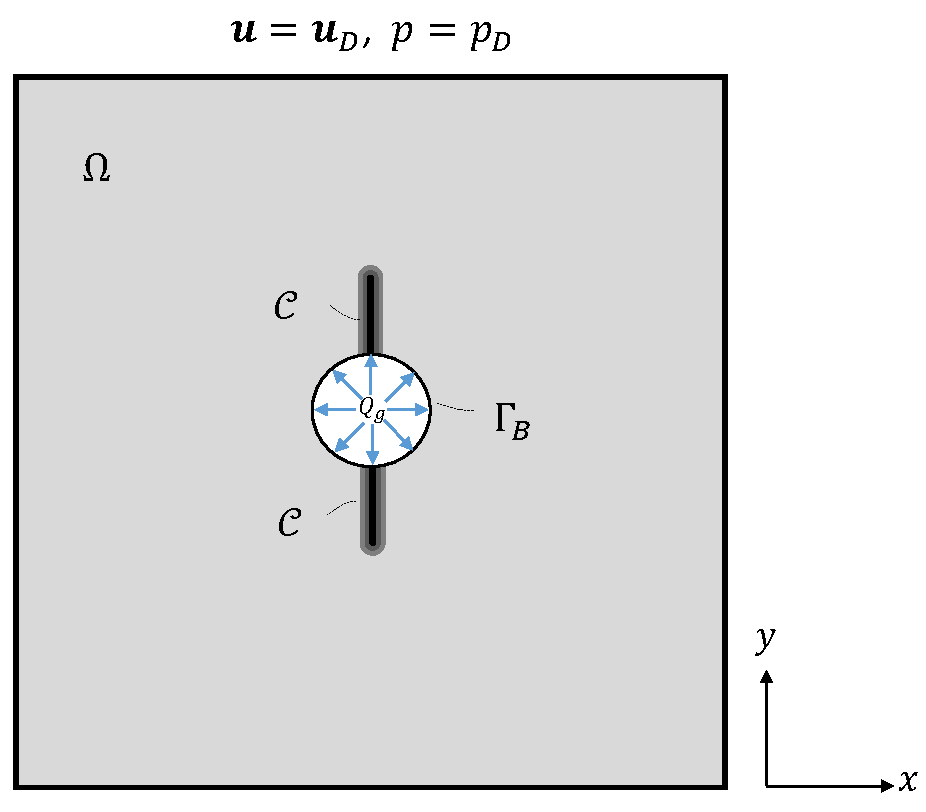
\includegraphics[width=0.8\textwidth]{omega_insitu2}
    \caption{Schematic of the computational domain. A square plate with a borehole placed inside is shown. The \emph{in situ} stress is applied on the external boundary, while the fluid is injected from the boundary of the borehole. The fracture $\mathcal{C}$ is approximated by a regularized crack surface $\mathcal{C}_{\ell}(d)$ which is a functional of the crack phase field.}
    \label{Fig:compute_domain}
\end{figure}

%\todo[inline]{YS: We have a conflict of notation for $\mu$. We need to use $G$ instead to represent the shear modulus.\\Vahid: Replaced.}

The variational approach to fracture is built on energy minimization with respect to the displacement field $\bm{u}:\Omega\rightarrow\mathbb{R}^2$ and its jump set, which we denote as $\mathcal{C}=\mathcal{C}(\bm{u})\subset\Omega$. Let $|\mathcal{C}|$ denote the one-dimensional Hausdorff measure of $\mathcal{C}$. Following Griffith's theory, the total potential energy of the fractured poroelastic solid is written as:
\begin{equation}\label{Eq:Pi}
    \begin{aligned}
        \Pi_{\mathcal{C}}[\bm{u},\mathcal{C}] &:= \int_{\Omega\setminus\mathcal{C}} \psi_0[\bm{\varepsilon}(\bm{u})] \; d\Omega
	    - \int_{\Omega} \bm{b} \cdot \bm{u} \; d\Omega
	    - \int_{\Gamma_N} \bm{t}_N\cdot \bm{u} \; d\Gamma \\
	    &- \int_{\Omega\setminus\mathcal{C}} \left(\alpha - 1\right)p\divergence\bm{u}\; d\Omega + 
	    \int_{\Omega\setminus\mathcal{C}}\nabla p\cdot \bm{u}\; d\Omega + g_c|\mathcal{C}|,\\
    \end{aligned}
\end{equation}
where $p$ denotes the pore pressure, $\alpha\in[0,1]$ is the Biot coefficient. {Constant} $g_c\in\mathbb{R}^+$ is the strain energy released per unit length of fracture extension. {The strain energy density $\psi_0[\bm{\varepsilon}(\bm{u})]$ is given by}
\begin{equation*}%\label{Eq:Strain_Energy}
    \begin{aligned}
        \psi_0(\bm{\varepsilon}) := \frac{\lambda}{2} (\trace \bm{\varepsilon})^2 + G \|\bm{\varepsilon}\|^2,
    \end{aligned}
\end{equation*}
with $\lambda$ and $G$ Lam\'e constants. These constants are related to Young's modulus $E$ and Poisson's ratio $\nu$ as $\lambda=E\nu/[(1+\nu)(1-2\nu)]$ and $G=E/[2(1+\nu)]$.
The linearized strain tensor takes the form:
\begin{equation*}
    \begin{aligned}
        \bm{\varepsilon}(\bm{u}) := 
        \frac{1}{2}\left(\nabla\bm{u}+\nabla\bm{u}^T\right).
    \end{aligned}
\end{equation*}
Finally, $\|\cdot\|$ denotes the Frobenius norm of a tensor.

\subsubsection{Regularized variational formulation of brittle fracture}
%\todo[inline]{YS: There is no need to explain $c_\omega$. Rather, its definition from $\omega(d)$ can be given instead. By the way, why $\omega$, not $w$?\\
%Vahid: I changed $\omega$ to $w$. Why not keeping the explanation of $c_w$? I kept it and also added its mathematical definition.}
%\Comment{YS: Do not use a backslash in the equation label.}
To develop a numerical method to approximate \eqref{Eq:Pi}, {the phase field approach replaces} the sharp-fracture description $\mathcal{C}$ with a phase field description, where the phase field is denoted as  $d:\Omega\rightarrow[0,1]$. In particular, regions with $d = 0$ and $d = 1$ correspond to the intact and fully broken materials, respectively. Using a phase field approach, the one-dimensional fracture $\mathcal{C}$ is approximated with the help of an elliptic %(Ambrosio-Tortorelli) 
functional \cite{ambrosio1990approximation, ambrosio1992approximation}:
\begin{equation}\label{Eq:Gamma_ell}
    \begin{aligned}
    \mathcal{C}_\ell[d]:=\frac{1}{4c_w}\int_\Omega\left(\frac{w(d)}{\ell} + \ell \nabla d\cdot\nabla d\right) d\Omega,  
    \end{aligned}
\end{equation}
where $\ell>0$ is the regularization length scale, which may also be interpreted as a material property, e.g., the size of the process zone. See Remark \ref{Rem:choice_ell} for comments on the choice of $\ell$. Constant $c_w=\int_{0}^{1} \sqrt{w(d)}$ is a normalization constant such that when $\ell\rightarrow 0$, {$\mathcal{C}_\ell[d]$} converges to the {length of the} sharp fracture{, $|\mathcal{C}|$}. Classical examples of $w(d)$ and $c_{w}$ are $w(d)=d^2$ and $c_{w}=1/2$ for the AT2 model, and $w(d)=d$ and $c_{w}=2/3$ for the AT1 model. Interested readers are referred to \cite{tanne2018crack,Bourdin2014014301} %\todo{YS: Wrong reference. The AT1 model came about in 2014 or so.\\Mostafa: Edited}~
for more elaborations.

%\todo[inline]{YS: We cannot use $\Pi$ for two different functionals. If the second one will be used more often, we can change the symbol for the first one, say $\Pi_{\text{sharp}}$.\\
%Vahid: Done. But the index `sharp' seems to me too long! I used $\Pi_{\mathcal{C}}$ instead. See \eqref{Eq:Pi}. Doesn't it look like better?}
%\todo[inline]{YS: See the new $\mathscr{S}_d$. I am still not clear about one thing: Do we impose $d\ge0$ or $d\ge$ its value at the previous time step?\\Vahid: OK. We impose $d\ge$ the previous value. The TAO solver gets a lower bound, and we update this bound every time step with the solution of $d$ from the last time step. Also, I changed $\mathscr{S}_d$ accordingly.}
On this basis, we replace \eqref{Eq:Pi} by a global constitutive dissipation functional for a rate independent fracture process \cite{BourdinCFRAC13}:
\begin{equation}\label{Eq:Dissipative_functional}
    \begin{aligned}
        \Pi[\bm{u},d] &:= \int_{\Omega} \psi[\bm{\varepsilon}(\bm{u}),d] \; d\Omega
	    - \int_{\Omega} \bm{b} \cdot \bm{u} \; d\Omega
	    - \int_{\Gamma_N} \bm{t}_N\cdot \bm{u} \; d\Gamma \\
	    &- \int_{\Omega}{\left(1 - d\right)}^2\left(\alpha - 1\right)p\divergence\bm{u}\; d\Omega + 
	    \int_{\Omega}{\left(1 - d\right)}^2\nabla p\cdot \bm{u}\; d\Omega \\
	    &+ \frac{g_c}{4c_{w}}\int_\Omega \left(\frac{w(d)}{\ell} + \ell \nabla d\cdot\nabla d\right)\;d\Omega,\\
    \end{aligned}
\end{equation}
where the admissible sets of displacement and phase field can be set as:
\begin{subequations}
\begin{align}
        \mathscr{S}_u &:= \left\{\bm{u} \in H^1\left(\Omega; \mathbb{R}^2\right) \middle|
        \bm{u} = \bm{u}_D \text{ on } \Gamma_D\right\}, \label{Su}\\
        \mathscr{S}_d &:= \{d\in H^1(\Omega)|0\le d\le 1\}.\label{Sd}
\end{align}
\end{subequations}
In practice, \eqref{Sd} will be used in combination with the irreversibility constraint, to be elaborated in Remark \ref{Rem:irreversibility}.
%\todo[inline]{YS: If we say ``Energy dissipation,'' then we have to give the dissipation rate. Otherwise we can say ``Degraded strain energy density'' or something of the sort.\\
%Vahid: I changed it to `Strain energy degradation'.}

%\todo[inline]{YS: Why not make these remarks as theorem-style environments? Then we do not need to number them by ourselves.
%\\ MM: I changed the style to theorem-style environment.}

%\todo[inline]{YS: The way I will organize the following paragraphs is perhaps first directly talk about Model A without mentioning even \eqref{Eq:psi}. Then Model B. As we do not have Model C here we do not need to be so general.\\
%Vahid: Following our discussion, I only kept the explanations for model B, now named as Amor's model.}

%\textsc{Remark 1} \textit{(Energy dissipation).}
%\todo[inline]{YS: See how I format the text that goes after ``Remark 1''}
\begin{remark}[Strain energy degradation]\label{Rem:psi}
The solid endures partial loss of stiffness due to the presence of fractures. In order to model this {effect}, the strain energy density is degraded with respect to the evolution of {the} phase field. Also note that as the damaged material responds differently to tension and compression, we let only a part of the strain energy density be degraded. For this purpose, we let the degraded strain energy in \eqref{Eq:Dissipative_functional} take the following general form:
\begin{equation*}%\label{Eq:psi}
\begin{aligned}
\psi(\bm{\varepsilon}, d) = g(d)\psi_+ + \psi_-,
\end{aligned}
\end{equation*}
where $g(d)$ satisfies $g(0)=1$, $g(1)=0$, and $g'(d)<0$ for all $d$ such that $0\le d\le 1$ \cite{Bourdin2000797}. A usual choice is $g(d)=(1-d)^2$. On the other hand, $\psi_{\pm}$ are such that
\begin{equation*}
    \begin{aligned}
        \psi_+(\bm{\varepsilon})+\psi_-(\bm{\varepsilon})=\psi_0(\varepsilon).
    \end{aligned}
\end{equation*}

Now since $\partial\psi/\partial d=g'(d)\psi_+$, only $\psi_+$ contributes to fracture propagation. 
\end{remark}

%\todo[inline]{YS: If we only do 3D or plane strain, we don't even need to mention what we do with the trace.\\
%Vahid: I omitted the relevant sentence. See below.}

%\deleted{Here we introduce two representative phase field models that differ in their choice of $\psi_+$.}

%\todo[inline]{YS: If we only use Amor \emph{et al.}'s model, we do not even need to say the name of the model.\\ Vahid: I deleted the relevant clause. See below}
There are several phase field models that differ in their choice of $\psi_{\pm}$. In this paper, we {adopt} the one proposed by Amor \emph{et al.}~\cite{Amor09}.
%\paragraph{Model A}
%\deleted{This is the original ''isotropic'' model \cite{Bourdin2000797}. It assumes the fracture responds similarly to tension and compression. It is convenient in that $\psi$ is continuous in both $\bm{\varepsilon}$ and $d$.}
%\paragraph{Model B} 
This model %\deleted{proposed by Amor \emph{et al.} \cite{Amor09}} 
assumes both volumetric expansion and deviatoric deformation contribute to fracture propagation, but volumetric compression does not. A decomposition of $\bm{\varepsilon}$ into volumetric and deviatoric parts reads:
\begin{equation*}
    \begin{aligned}
        \vol\bm{\varepsilon} := \frac{1}{3} (\trace\bm{\varepsilon}) \mathbf{1}, \quad
        \dev\bm{\varepsilon} := \bm{\varepsilon} - \vol\bm{\varepsilon}.
    \end{aligned}
\end{equation*}
%\deleted{where the trace operator is understood in three dimensions for both two-dimensional plane strain and plane stress cases.}

%\todo[inline]{YS: An alternative way to handle the irreversibility constraint is to use a history variable. Shall we mention it too?\\
%Vahid: I added a paragraph and mentioned this approach by Miehe as an alternative way.\\
%YS: Nice try, but it looks too long. We only need to say that a history field can be used for enforcing irreversibility. Moreover, although this point does not need to appear in the paper, the same concept of history variable can be used for Amor's model as well, without changing the way of tension-compression decomposition.\\
%Vahid: I have summarized the text now.}

%\textsc{Remark 2} \textit{(Irreversibility constraint).}

\begin{remark}[Irreversibility constraint]\label{Rem:irreversibility}
%With reference to \eqref{Eq:psi}, the minimum requirement on $g(d)$ is $g(0)=1$, $g(1)=0$, and $g'(d)<0$ for all $d$ such that $0\le d\le 1$ \cite{Bourdin2000797}. 
The requirement $g'(d)<0$ comes from the underlying irreversibility condition (the fracture can never heal) in time:
\begin{equation}\label{Eq:irreversibility}
    \partial_t d\geq 0.
\end{equation}
Consequently, modeling of fracture evolution problems leads to {inequality constraints, and sometimes gives rise to a variational inequality formulation}.

As an alternative way to {model} the irreversibility, Miehe \emph{et al.}~\cite{Miehe20102765} proposed a phase field model based on a local history field. In this model, the evolution of the phase field $d$ is driven by the historically maximum value of $\psi_+$ at the point of interest.
%{This model assumes that both volumetric expansion and deviatoric deformation contribute to the crack propagation but not volumetric compression.} 
%\added{In this model, the evolution of the phase field $d$ is defined as:}
%\begin{equation}\label{eq:18}
%\partial_t d=\frac{1}{\eta}\left\langle 2\left(1-d\right)H-\frac{g_c}{l}\left(d-l^2\Delta d\right)\right\rangle_+,
%\end{equation}
%\added{where $\eta>0$ is the \textit{artificial viscosity}, a material parameter to be input, $\langle a \rangle_\pm := (|a|\pm a)/2$ for all $a\in\mathbb{R}$, and}
%\begin{equation*}
%H(\bm{x},t) := \max_{s\in[0,t]} \psi_+(\bm{\varepsilon}(\bm{x})), \quad
%\psi_+(\bm{\varepsilon})= \frac{\lambda}{2} \langle \trace \bm{\varepsilon} \rangle_+^2 + \mu\sum_{i=1}^2 \langle\varepsilon_i\rangle_+^2
%\end{equation*}
%\added{is the historical maximum value of the tensile strain energy density of the point of interest.}
\end{remark}

%\todo[inline]{Vahid: I read somewhere by Bourdin \emph{et al.} that it has been shown the residual stiffness parameter $k$ has no significant impact on the numerical solution. Shall we omit this remark then?\\
%YS: If we used $k$, then just keep the remark. If not, then delete $k$ everywhere and this remark.}
%\begin{remark}[Residual stiffness]
%An additional small number $k$ with {$0<k\ll 1$} is added to the degradation function $g(d)$%coefficient of $\psi_+(\bm{\varepsilon})$
%, i.e., having $[(1-d)^2+k]$ instead of $(1-d)^2$ in \eqref{Eq:Dissipative_functional}, to prevent the lack of stiffness for completely fractured portions of the solid \cite{Bourdin2000797}. Here, we take $k=1\times10^{-12}$.
%\end{remark}
%\todo[inline]{
%YS: Equation \eqref{Eq:choice_ell} or something similar was proposed in 2014 by Bourdin.\\
%YS: I believe we should not stop here. We need to know what led to the two different expressions -- the different types of loading?\\Vahid: Now I find the formula by Bourdin \emph{et al.} \cite{Bourdin2014014301} suits more for our case, since it is for AT1 models in spite of the other work by Borden \emph{et al.} \cite{Borden2012A}. The details on how they end up with \eqref{Eq:choice_ell} is given in \cite{Bourdin2014014301}.\\
%Another point: As we have already defined $\lambda$ and $G$ at this point, we need to introduce $E$ in terms of $\lambda$ and $G$. Or we should have defined $\lambda$ and $G$ in terms of $E$ and $\nu$.
%\\Vahid: I put the conversion formula for $E$ in below.}
\begin{remark}[The choice of $\ell$]\label{Rem:choice_ell}
{Based on an analytical solution for the critical tensile strength $\sigma_\text{cr}$ that a one-dimensional bar can sustain \cite{Bourdin2014014301}, we use the following equation for the choice of $\ell$:}
\begin{equation}\label{Eq:choice_ell}
    \begin{aligned}
        \ell=\frac{3Eg_c}{8\sigma_\text{cr}^2},
    \end{aligned}
\end{equation}
where $E$ and $g_c$ can be obtained from regular experiments, while $\sigma_\text{cr}$ can be approximated by the tensile strength $\sigma_t$. Assuming all {other} parameters are known, the formula \eqref{Eq:choice_ell} is able to estimate $\ell$, though the accuracy is unknown for more complex cases.
\end{remark}
%\todo[inline]{YS: Maybe we don't need this subsubsection at all.\\Vahid: Or shall we move it to \ref{sub:weak_form}?\\
%YS: The problem with the EL equations is that they hold only when the equality holds, while we are solving a constrained minimization problem. Wherever the constraint $d\le 0$ or $d\ge 1$ is in place, the corresponding EL \eqref{Eq:Euler_d} does not holds.
%\\Vahid: OK. So the EL subsection does not exist anymore.}
%\subsubsection{The Euler-Lagrange equations}
%%\todo[inline]{YS: These spaces should be introduced as constraints for the optimization problem with \eqref{Eq:Dissipative_functional}.
%%\\Vahid: Now they are placed right after \eqref{Eq:Dissipative_functional}.}
%
%%\todo[inline]{YS: I got $-\mathbf{b}$ instead of $\mathbf{b}$ in \eqref{Eq:Euler_u}.\\
%%Vahid: Correct. Not it's changed.}
%
%The Euler-Lagrange equations of \eqref{Eq:Dissipative_functional} are obtained by {taking} the first variations with respect to $\bm{u}$ and $d$ {followed by appropriate integrations by parts}, and are expressed as follows:
%\begin{subequations}\label{Eq:Euler}
%    \begin{align}
%         \label{Eq:Euler_u}  {-}\divergence\bm{\sigma} - \mathbf{b} +
%        \left(\alpha-1\right) \nabla  \left[ (1-d)^2 p\right] + \left(1-d \right)^2 \nabla p &= \mathbf{0}, \quad  \text{in~} \Omega, \\
%        \label{Eq:Neu_u} \bm{\sigma}\cdot\bm{n} - \bm{t}_N &= \bm{0}, \quad \text{on~} \Gamma_N, \\
%        \begin{split}
%                  \label{Eq:Euler_d} \frac{\partial\psi}{\partial d} + \frac{g_c}{4c_{w}\ell}\left({w}'(d) - {\ell}^2 \Delta d\right)
%        + 2 \left(\alpha-1\right) \left(1-d \right)p\divergence \bm{u}
%        \\- 2\left(1-d\right)\nabla p\cdot\bm{u} &= 0, \quad  \text{in~} \Omega, 
%        \end{split}
%          \\
%        \label{Eq:Neu_d} \frac{\partial d}{\partial \bm{n}} &= 0, \quad  \text{on~} \partial\Omega,
%    \end{align}
%\end{subequations}
%where
%\begin{equation*}
%    \begin{aligned}
%        \bm{\sigma} =\frac{\partial\psi}{\partial\bm{\varepsilon}} = g(d) \bm{\sigma}_+(\bm{\varepsilon}) + \bm{\sigma}_-(\bm{\varepsilon})
%    \end{aligned}
%\end{equation*}
%is the Cauchy stress with $\bm{\sigma}_\pm(\bm{\varepsilon}):=\partial\psi_\pm/\partial\bm{\varepsilon}$, and $\bm{n}$ is the unit outer normal to $\partial\Omega$. Here \eqref{Eq:Euler_u} expresses the momentum conservation of the solid, \eqref{Eq:Euler_d} defines the phase field evolution, and \eqref{Eq:Neu_u} and \eqref{Eq:Neu_d} are Neumann boundary conditions for $\bm{u}$ and $d$, respectively.

\subsection{Carbon dioxide as a compressible fluid} \label{Sec:CO2}
The governing equations for the fluid flow in a porous medium are given by mass conservation, momentum balance, and the equation of state.
The mass conservation equation reads:
\begin{equation}\label{Eq:Mass_Conserv}
    \begin{aligned}
        \partial_t\left(\phi\rho\right)  +\nabla\cdot\left(\rho\bm{q}\right)&=0  \quad  &\text{in~} \Omega, \\
    -\rho\bm{q} \cdot n &=Q_g  \quad  &\text{on~} \Gamma_B.       
    \end{aligned}
\end{equation}
Here $\phi$ denotes the porosity of the porous medium (the fraction of volume occupied by the fluid), $\rho$ the density of the fluid, $\bm{q}$ the Darcy velocity vector, and $Q_g$ the fluid source. Note that $Q_g$ has the unit of volumetric flow rate per unit volume. Also, we assume the rock is saturated by the fluid so that the fluid content in rock per volume is expressed by $\phi\rho$.

%\todo[inline]{YS: Do we have the last term of \eqref{Eq:Darcy_law} in the numerical model or not? If not, then we do not need it in the equation, just mention it in the text.\\
%Vahid: No, we don't use this term. I deleted it then. I prefer we even not mention it in the text, as some other references do. Now I mentioned it though. See below.\\
%YS: Is it because $z$ is the direction perpendicular to our plane of interest? If so, it is easy to justify.\\Vahid: Yes, it is.}

In addition to \eqref{Eq:Mass_Conserv}, we state the momentum balance in the form of Darcy's law. This law indicates a linear relationship between the fluid velocity and the head pressure gradient:
\begin{equation}\label{Eq:Darcy_law}
    \begin{aligned}
        \bm{q} = -\frac{k}{\mu} \nabla p,
    \end{aligned}
\end{equation}
where $k=k(d)$ is the permeability of the rock, and $\mu$ is the dynamic fluid viscosity. %\replaced{}{$g$ is the magnitude of the gravitational acceleration, and $z$ is the depth} 
Note that there could be an additional term $- \rho g\nabla z$ %\todo{YS: $\nabla z$? It is a valid definition but $\nabla z=\bm{e}_z$ (the unit vector in the $z$-direction. Is it just $z$?)\\Vahid: I believe it is $\nabla z$, and since in our case $|\nabla z|=1$, hence $\rho g \nabla z$ is much smaller than the magnitude of the other vector, i.e., $\nabla p$.} 
on the right hand side of \eqref{Eq:Darcy_law}, where $g$ and $z$ are the magnitude of the gravitational acceleration and the depth, respectively. This term is, however, in our case negligible, as we assume an almost horizontal computational domain.
%Note the effect of the second term ($\rho g\nabla z$) is negligible.
Also, we assume the porosity is not dependent on the stress condition. On the other hand, we correlate the permeability to the phase field value by:
\begin{equation}\label{Eq:k_0}
    \begin{aligned}
        k(d) = k_0\exp{\left({\alpha}_k d\right)},
    \end{aligned}
\end{equation}
where $k_0$ is the permeability of the intact material, and ${\alpha}_k$ is a coefficient to indicate the effect of phase field evolution on the permeability. We take ${\alpha}_k=7.0$ (see \cite{PILLAI201836, ZHU2013179} for more description). Figure \ref{Fig:Permeability_increments} illustrates the permeability increasing with respect to the evolution of the phase field variable.

%\todo[inline]{YS: How about changing the vertical axis of Figure \ref{Fig:Permeability_increments} to $k(d)$?\\Mostafa: Done.}

\begin{figure}[htbp]
    \centering
    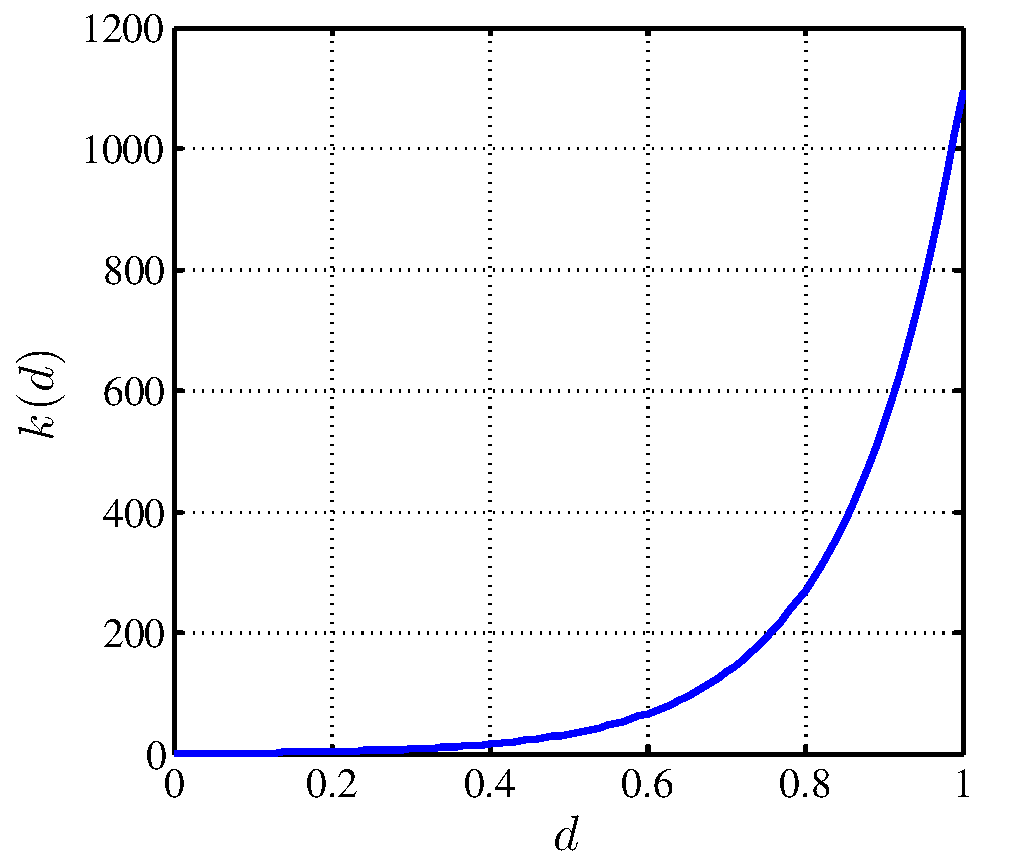
\includegraphics[width=0.6\textwidth]{permeability}
    \caption{Plot of $k(d)=\exp(7.0 d)$, permeability, as a function of the phase field variable $d$.}
    \label{Fig:Permeability_increments}
\end{figure}

The first term on the left hand side of \eqref{Eq:Mass_Conserv}, the rate of change of fluid content, can be written as:
\begin{equation}\label{Eq:diff_m}
    \begin{aligned}
        \partial_t\left(\phi\rho\right) = \rho \; \partial_t \phi +\phi \; \partial_t \rho  = \rho \;  \partial_t \varepsilon_v{+\phi \; \partial_t \rho},
    \end{aligned}
\end{equation}
where we have assumed the rate of change of pore volume is equal to that of the volumetric strain, which is given by $\varepsilon_v= \nabla \cdot \bm{u}$. 

%\todo[inline]{YS: I find the derivation of \eqref{Eq:Darcy_right} is exact. Where did we neglect the quadratic gradient term? Or \emph{will} we? Then we need to add one more step with $\doteq$ or $\approx$ at the end.\\
%Vahid: Yes, the derivation was exact. I also added the approximation to the equation. But note in the implementation/code, we neglect the quadratic term. I changed the text and equation accordingly.\\
%YS: But the exact derivation would have a term with $\nabla k$, or equivalently, $k'(d)\nabla d$.\\
%Another point: What is the justification for us to neglect the quadratic term? Is it because $p$ is the fluctuation value above some constant reference value?\\Vahid: Finally we came up with \eqref{Eq:General_pressure}.}

%\todo[inline]{YS: Shall we multiply \eqref{Eq:Darcy_right} by $-1$?\\Vahid: Not existed anymore.}
%\deleted{Also, with \eqref{Eq:Darcy_law}, the first term of the right hand side of \eqref{Eq:Mass_Conserv} is computed as:}
%\begin{equation}\label{Eq:Darcy_right}
%    \begin{aligned}
%        \nabla\cdot\left(\deleted{-}\rho\frac{k}{\mu}\nabla p\right) = \nabla\left(\deleted{-}\rho\frac{k}{\mu}\right)\cdot\nabla p  \replaced{+}{-} \rho\frac{k}{\mu}\Delta p &= \deleted{-}\frac{k}{\mu}\left[ \frac{d\rho}{dp} \left|\nabla p\right|^2 + \rho \Delta p\right]\\&\doteq\deleted{-}\frac{k}{\mu}\rho\Delta p
%    \end{aligned}
%\end{equation}
%\begin{equation}\label{Eq:Darcy_right}
%\begin{aligned}
%\nabla\cdot\left(\deleted{-}\rho\frac{k}{\mu}\nabla p\right) = \nabla\left(\deleted{-}\rho\frac{k}{\mu}\right)\cdot\nabla p  \replaced{+}{-} \rho\frac{k}{\mu}\Delta p &= \deleted{-}\frac{k}{\mu}\left[ \frac{d\rho}{dp} \left|\nabla p\right|^2 + \rho \Delta p\right]+\added{\frac{\rho}{\mu}\nabla k\cdot\nabla p}\\&\deleted{\doteq\deleted{-}\frac{k}{\mu}\rho\Delta p}
%\end{aligned}
%\end{equation}
%\begin{equation}%\label{Eq:Darcy_right}
%    \begin{aligned}
%        \nabla\cdot\left(-\rho\frac{k}{\mu}\nabla p\right) = \nabla\cdot\left(-\rho\frac{k}{\mu}\right)\nabla p  - \rho\frac{k}{\mu}{\nabla}^2 p = -\frac{k}{\mu}\left[ \frac{d\rho}{dp} \left(\nabla p\right)^2 + \rho{\nabla}^2 p\right]
%    \end{aligned}
%\end{equation}
%\deleted{Note that for sake of simplicity, {in our implementation} we neglect the quadratic gradient term of pressure $|\nabla p|^2$ {in \eqref{Eq:Darcy_right}}.
%}
%\todo[inline]{YS: There are many parameters like $d_i$, $t_i$, etc., undefined in \eqref{Eq:Res_Helmholtz}. Maybe we can say they are given in \cite{span1996new}.\\ Vahid: We already referred the readers for the many parameters. See ``Interested readers\dots'' now in blue.\\
%YS: Well, not just interested readers. The information is not complete for readers to reproduce our results. We need to give the numbers of all these parameters. Explanation is optional, though.\\Vahid: How does it look like now?}

Under isothermal conditions, the gas density varies significantly with pressure. This is {captured} by an equation of state (EOS). One applicable EOS for CO$_2$ is known as the Span-Wagner (S-W) equation \cite{span1996new} defined in terms of the Helmholtz free energy. The CO$_2$ density and pressure are related by:
\begin{equation}\label{Eq:Density_Pressure}
    \begin{aligned}
        p=\left(1+\delta\varphi^r_{\delta}\right)\rho RT,
    \end{aligned}
\end{equation}
where $R$ is the universal gas constant, and $\varphi^r_{\delta}$ is the derivative of the residual part of the full expression of Helmholtz energy $\varphi^r$ with respect to the reduced density $\delta$, with %. It is written as:
\begin{equation}\label{Eq:Res_Helmholtz}
    \begin{aligned}
        \varphi^r\left(\delta,\tau\right) &= \sum_{i=1}^{7} n_i  \delta^{d_i}\tau^{t_i}+\sum_{i=8}^{34} n_i\delta^{d_i} \tau^{t_i} e^{-\delta^{c_i}}+ \sum_{i=35}^{39} n_i  \delta^{d_i}\tau^{t_i} e^{-\alpha_i\left(\delta-\varepsilon_i \right)^2-\beta_i\left(\tau-\gamma_i\right)^2}\\ &+\sum_{i=40}^{42} n_i\Delta^{b_i}\delta e^{C_i\left(\delta-1\right)^2-D_i\left(\tau-1\right) ^2},\\
    \end{aligned}
\end{equation}
in which
\begin{equation*}\label{Eq:Delta}
    \begin{aligned}
        \Delta=\left\lbrace\left(1-\tau \right)+A_i\left[\left(\delta-1 \right)^2\right]^{\dfrac{1}{2\beta_i}}\right\rbrace ^2+B_i\left[\left(\delta-1 \right)^2\right]^{a_i}.
    \end{aligned}
\end{equation*}
In \eqref{Eq:Res_Helmholtz}, $\rho_c$ and $T_c$ are the critical density and temperature, respectively, and $\delta=\rho/\rho_c$ and $\tau=T/T_c$ are the reduced ones. For the sake of brevity, here we do not provide the definitions and values of other parameters in \eqref{Eq:Res_Helmholtz}, but refer the readers to \cite{span1996new}.

%\todo[inline]{YS: It looks more natural for \eqref{Eq:Density_Pressure} to come before \eqref{Eq:Res_Helmholtz}, otherwise it seems a puzzle why we need the latter.\\Mostafa: Done}

%\todo[inline]{YS: ``$\delta \varphi^r_{\delta}$ and $\delta^2 \varphi^r_{\delta \delta}$ are the first and second derivatives of $\varphi^r$ with respect to $\delta$, respectively'' seriously? It looks like $\varphi^r_{\delta}$ and $\varphi^r_{\delta \delta}$ are the first and second derivatives of $\varphi^r$ with respect to $\delta$, respectively. By the way, why do we keep the superscript $r$ all along?\\
%Vahid: You're right about the derivatives of $\varphi^r$. I changed the text accordingly. Regarding the superscript $r$, as we denote by $\varphi^r$ the `residual' part, I preferred to keep it. And also it is easier for the reader to follow as she finds the same notation in other references.}

%\todo[inline]{YS: Is $k/\mu$ constant or not? I felt the derivation of \eqref{Eq:Darcy_right} can only go through in the case of yes. Then in \eqref{Eq:General_pressure} why did we move it back inside the parentheses instead of writing $-(k/\mu) \Delta p$?\\
%Vahid: Actually no. $k/\mu$ is not constant as $k$ is a function of $d$. However, I find that the derivation of \eqref{Eq:Darcy_right} is still correct. I put $-(k/\mu)\rho\Delta p$ in \eqref{Eq:General_pressure}.}

By substituting  \eqref{Eq:Darcy_law},\eqref{Eq:k_0}, \eqref{Eq:diff_m}, and \eqref{Eq:Density_Pressure} in \eqref{Eq:Mass_Conserv}, the governing equation for CO$_2$ flow is written as follows: 
%\begin{equation}\label{Eq:General_pressure}
%    \begin{aligned}
%        \frac{\phi}{{N}} \partial_t p +\rho \; \partial_t \varepsilon_v -\frac{k}{\mu}\left[\frac{d\rho}{dp}\rho\Delta p\right] =Q_g,
%    \end{aligned}
%\end{equation}
\begin{equation}\label{Eq:General_pressure}
\begin{aligned}
\phi \; \partial_t \rho+\rho \; \partial_t \varepsilon_v -\nabla \cdot \left( \rho \frac{ k(d)}{\mu} \nabla p \right) =0,  \quad  &\text{in~} \Omega,\\
    \rho\bm{q} \cdot n =-Q_g,  \quad  &\text{on~} \Gamma_B,\\
    p = p_D, \quad &\text{on~}\Gamma_P,
\end{aligned}
\end{equation}
where $\Gamma_P=\partial\Omega\setminus\Gamma_B$. 
%\todo[inline]{YS: If the fluid is incompressible, then we should have $K_f=\infty$, right?\\
%Vahid: Yes.\\
%YS: Then why do we not take away the term $\phi/K_f$ as it vanishes?\\
%Vahid: We finally agreed to delete this part.}
%In the rock mechanics, we usually use the mulation of Detournay \cite{detournay1995fundamentals} (Table 2, page 123) related to "\textbf{Invariance of porosity under $\Pi$-loading}"   while for "\textbf{Incompressible fluid and solid constituents}" (page 122) you are right $K_f \rightarrow \infty$ }

%\paragraph{\deleted{Incompressible fluid flow}} \deleted{Here, it is also worth mentioning the case of incompressibility. For the incompressible fluid flow, the left-hand-side of \eqref{Eq:Mass_Conserv} reads} \cite{detournay1995fundamentals}:
%\begin{equation}\label{Eq:Mass_Left}
%    \begin{aligned}
%       \deleted{ \partial_t \left(\phi\rho\right) =
%        \phi \; \partial_t  \rho+ \rho \; \partial_t \phi
%        = \rho\left(\frac{\phi}{K_f}+\frac{\alpha -\phi}{K_s}\right)
%       \partial_t p + \alpha\rho \;  \partial_t \varepsilon_v,}
%    \end{aligned}
%\end{equation}
%\deleted{where $K_f$, $K_s$ are the bulk modulus of fluid and rock grains, respectively. 
%Combining Eqs.~\eqref{Eq:Mass_Conserv}-\eqref{Eq:Mass_Left}, the generalized equation of the incompressible fluid flow is obtained as follows:}
%\begin{equation}\label{Eq:Mass_General}
%    \begin{aligned}
%        \deleted{\left(\frac{\phi}{K_f}+\frac{\alpha -\phi}{K_s}\right) \partial_t p+  \alpha \; \partial_t \varepsilon_v+\nabla \cdot \left( -\frac{k}{\mu}\nabla p\right) =Q_g.}
%    \end{aligned}
%\end{equation}

%\todo[inline]{YS: Here we need to summarize a non-redundant collection of equations.\\Vahid: Added below.\\
%YS: It is still not clear that for the solid it is a constrained minimization problem.\\Vahid: More descriptions are added now.}
%\todo[inline]{YS: Comparing $\mathscr{S}_p$ and $\mathscr{S}_u$, does it mean $p$ and $\bm{u}$ will always be imposed on the same part of $\partial\Omega$, called $\Gamma_D$? By the way, why do we need the admissible pressure for the strong form? I added the corresponding boundary condition instead. Please confirm.\\Vahid: Now I defined $\Gamma_P$ for $p_D$. The admissible pressure is moved to \ref{sub:weak_form}.}
\paragraph{Summary of governing equations} The governing equations for modeling the CO$_2$ fracturing are summarized as follow: for the porous medium deformation, the functional defined in \eqref{Eq:Dissipative_functional} is minimized among $(\bm{u},d)\in \mathscr{S}_u\times\mathscr{S}_d$ under the constraint \eqref{Eq:irreversibility}, while %The lower bound $d^{n-1}$ is considered to ensure the irreversibility of the fracture. 
for the compressible fluid the boundary value problem \eqref{Eq:General_pressure} is used to solve for the pressure $p$.

Note also that $d\equiv0$, i.e., there is no preexisting crack in the specimen and we do not allow for any nucleation of the fracture as the rock strength is assigned a very large value.

\section{Numerical solution}\label{sec:Num_Sol}
In this section we present an algorithm that adopts standard procedures to obtain a numerical method to solve the initial boundary value problem presented in Section \ref{sec:Math_model}. %\deleted{In the sequel we will introduce the discrete formulations in {Sections\ref{sub:weak_porous} and \ref{sec:CO2-discretization}, for the porous medium and fluid flow respectively. Note that we adopt a staggered approach to solve the coupled problem.}
%\subsection{Porous medium}
%\deleted{Here, to facilitate the numerical computation with the FEM, in \ref{sub:weak_porous} we first state the weak form. Then in \ref{sub:spatial_porous} we present the spatial discretization for the porous medium.}
%\deleted{We choose $0=t_0<t_1<\ldots<t_N=\replaced{t_f}{T}$ and seek the solution at these discrete instants. We will adopt the backward Euler method for time discretization. Now we detail how we advance from time step $n-1$ to $n$. For later convenience, let $\Delta t_n := t_n - t_{n-1}$ for $n=1,\ldots,N$. \added{As we use the same time steps,} when there is no risk of confusion, the subscript $n$ will be dropped. \replaced{It implies}{Moreover,} the field $p$ will wear a superscript $n-1$ if it refers to the solution at $t_{n-1}$, but will have no superscript if it refers to the solution at the current time step, i.e., $t_n$.} % With this specific, \eqref{Eq:General_pressure} is discretized as:
%\subsection{\deleted{Numerical algorithm}}\label{sec:Num_algo}
%\todo[inline]{YS: It is more appropriate to make Section \ref{sec:Num_algo} a subsection of Section \ref{sec:Num_Sol}.\\
%Vahid: Now it is a subsection.}
%\todo[inline]{YS: There is no clear cut comparison between monolithic and staggered approaches. Why don't we just mention how we do it and avoid commenting on the monolithic approach?\\Vahid: I agree the advantage is not so clear, but shouldn't we justify why we chose the staggered algorithm then? Now I deleted the comparison part though. See below.}
In this algorithm, a staggered approach is employed to solve the underlying equations, i.e., the solution is obtained via iteration between the variables \cite{Bourdin2000797,bourdin2008variational}. This idea is based on the fact that by fixing two variables, the problem becomes convex in the remaining unknown. However, one drawback for such an approach is that it might need many iterations to achieve convergence among the three fields.

For the problem at hand, we need to solve a coupled system consisting of mass balance for the compressible fluid and a dissipative potential energy with the phase field. We provide a fully iterative approach in which at each stage we solve for one unknown while the other two variables are fixed to their values at the last iteration. Readers are referred to Algorithm \ref{Alg:Co_2_fracking} for complete elaboration.

\RestyleAlgo{algoruled} 
\LinesNumbered
\begin{algorithm}[htbp]
	\caption{Algorithm for modeling the CO$_2$ by phase field.} \label{Alg:Co_2_fracking}
	
	\KwIn{  $p_{0}$, $d_{0}$, $\bm{u}_0$, $\rho_0$, and $\varepsilon_{\text{tol}}$}
	\KwOut{  $p_n$, $d_n$, and $\bm{u}_n$, $n= 1, \cdots,N $}
	
	%Construct $d$-field, $d_0$;\\
	Set flow and mechanical boundary conditions $\sigma_1$, $\sigma_3$, and $Q_g$;\\
	%Set $n=1$;\\
	
	\For()
	{ {$n= 1 ~ to~ N$};  }{Set  $t=n\Delta t$ and $k=0$; \tcc{$k$ is an iteration counter}
		
		{\Repeat( ){$\varepsilon_d=\left\| d_n^{\left( m\right) }-d_{n}^{\left( m-1\right) } \right\|_{2}  <\varepsilon_{\text{tol}}$ }
			{ 
				$m=0$; \tcc{$m$ is another iteration counter}
				
				
				
				
				{\Repeat( ){   $\left\| p_n^{\left( k\right) }-p_{n}^{\left( k-1\right) } \right\|_{2}  <\varepsilon_{\text{tol}} ~\textbf{and}~ \left\| \bm{u}_n^{\left( k\right) }-\bm{u}_{n}^{\left( k-1\right) } \right\|_{2}  <\varepsilon_{\text{tol}}$  }
					{
						Step - P: compute $p_n$ with \eqref{Eq:weak_pressure};\\
						Step - U: compute $\bm{u}_{n}$ with \eqref{Eq:Residual};\label{line:compute_u}\\
						
						
						
						Update $ \rho_n^{\left( k+1\right) } \leftarrow \rho(p_n^{\left( k\right) })$ with \eqref{Eq:Density_Pressure};\\
						
						$k+1 \leftarrow k$
					}
				}
				
				
				Step - d: compute $d_n$ with \eqref{Eq:Residual}; \\
				$m+1 \leftarrow m$
			}
		}
		
		$\bm{u}_{n-1} \leftarrow \bm{u}_n$;\\ 
		$p_{n-1} \leftarrow p_n$;\\ 
		$\rho_{n-1} \leftarrow \rho_n$;\\ 
		%$n+1 \leftarrow n$
	}
	
\end{algorithm}
%\todo[inline]{YS: $d\in[0,1]$ is a wrong way to write it. The correct way is $0\le d\le 1$. Because $d$ is a function, not a single real number.\\
%Vahid: OK. So you have fixed it.}

%\todo[inline]{YS: How do we know we are using the active set method? Even if yes, why do we need to explain such a classical one? I tend to believe no; we should just mention the algorithm(s) within FEniCS we have chosen for the constrained minimization.\\Vahid: I removed the whole paragraph then. Where we name the TAO solver, I just mentioned that the solver itself imposes the lower bound.}
%
%\deleted{To ensure that $0\le d\le 1$ and also the inequality constraint \eqref{Eq:irreversibility} are imposed on the phase field, there are mainly three kinds of approaches: (a) the active-set method, (b) the penalty method \cite{gerasimov2015line} and (c) the augmented Lagrangian method \cite{Wheeler201469}. Now we briefly explain the active-set method, which we use: For each loading step, one needs to check the constraints after the stopping criterion for iteration is achieved. If no constraint is violated, then continue the computation for the next load step; otherwise, find those points that violate the constraints and set them to the appropriate upper or lower bounds for further iteration until all the constraints are satisfied.}
%
%%\todo[inline]{YS: As we have cited \cite{Logg2012}, there is no need to explain so much about FEniCS. Just keep the essence, which is the 3rd sentence below. Also ``takes care of'' is too colloquial for a paper.\\
%%	Vahid: Now I deleted the auxiliary explanations.\\
%%	YS: I objected the advertisement-like wordings for FEniCS. I changed them to neutral ones. Still I prefer simplifying the description by saying that all we need to input are the functional and its first and second derivatives and the constraints.}

We implement our method on FEniCS, an open-source finite element software \cite[pp.~173--225]{Logg2012}. Therein, the user merely needs to provide the variational form of the problem as well as the geometry and mesh information. Then, a big advantage of FEniCS is that the software itself completes all steps toward generating the global stiffness matrix.

%\todo[inline]{YS: Why don't we use line numbers to explain? Vahid: I included the line numbers for the code. The explanations are also modified accordingly.}

%\todo[inline]{YS: The upcoming three paragraphs are NOT coherent, although individually well written. Put more thoughts on their order and necessary link words.\\Vahid: It should look better now.}

Below we show an excerpt of the used FEniCS code. This piece of code performs some calculations for line \ref{line:compute_u} in Algorithm \ref{Alg:Co_2_fracking} wherein $\bm{u}$ is solved for while the other two unknowns are fixed. It first defines $\bm{\varepsilon}$, $\psi_0$, and $\psi(\bm{\varepsilon},d)$ in lines 1, 3, and 5, respectively. Then, the standard finite element shape functions are defined in line 8, and the admissible function space (\texttt{TrialFunction}), the test function space (\texttt{TestFunction}), and the unknown function $\bm{u}$ (\texttt{Function}) are defined in line 9. Afterwards, the elastic energy is introduced as a variational form in line 11. Finally, in lines 12 and 13, the code takes the first variation $\delta\Pi[(\bm{u},d);\Bar{\bm{u}}]$ \eqref{Eq:Residual_u} and the second variation $\delta^2\Pi[(\bm{u},d);\Bar{\bm{u}};\delta\bm{u}]$ \eqref{Eq:Tangent_u} and builds the nodal residual vector as \texttt{Residual\_u} and the tangent stiffness matrix as \texttt{Jacobian\_u}.
\begin{lstlisting}
def eps(u_):
return sym(grad(u_))
def psi_0(u_):
return  0.5 * lmbda * tr(eps(u_))**2 + mu * eps(u_)**2
def psi_(u_, d_):
return ((1 - d_)**2 + k_ell) * psi_0(u_)

V_u = VectorFunctionSpace(mesh, "CG", 1)
u_, u, u_t = Function(V_u), TrialFunction(V_u), TestFunction(V_u)

energy_elastic = psi_(u_, d_) * dx
Residual_u = derivative(energy_elastic, u, u_t)
Jacobian_u = derivative(Residual, u_, u_t)
\end{lstlisting}



%\todo[inline]{YS: This is too lengthy, and ``pick up'' is too colloquial.\\Vahid: Replaced by a more brief paragraph.}
To solve the three unknowns, we select for $\bm{u}$ and $p$ the linear solver MUMPS which is convenient for solving large linear systems \cite{amestoy2000mumps}, and for $d$ the TAO optimization solver integrated into the PETSc library \cite{munson2014toolkit, petsc-user-ref}, which has the capability of solving inequality constrained optimization problems as the one at hand. Interested readers are referred to \cite{bilgen2018phase} for more information about the applied solvers.
%{As we solve for each unknowns separately, we can choose different solvers. Thus, for $\bm{u}$ using Newton's method, we pick up a linear solver like MUMPS which is convenient for the solution of large linear systems \cite{amestoy2000mumps}. For $d$, however, \eqref{Eq:Euler_d} is solved using the TAO optimization solver which is integrated into the PETSc library \cite{munson2014toolkit}, \cite{petsc-user-ref}. The fluid flow sub problem is also solved with standard Newton's method with MUMPS. Interested readers are referred to \cite{bilgen2018phase} for more elaborative information about the used solvers.}
%{As we solve for each unknowns separately, we can choose different solvers. Thus, for $\bm{u}$ using Newton's method, we pick up a linear solver like MUMPS which is convenient for the solution of large linear systems \cite{amestoy2000mumps}. For $d$, however, \eqref{Eq:Euler_d} is solved using the TAO optimization solver which is integrated into the PETSc library \cite{munson2014toolkit, petsc-user-ref}. The fluid flow sub problem is also solved with standard Newton's method with MUMPS. Interested readers are referred to \cite{bilgen2018phase} for more elaborative information about the used solvers.}
%\todo[inline]{Mostafa: The statement below is deleted since we update the parameters in each iteration according to the pressure in the last iteration, not last time step.}
%\deleted{To end this session, it is also worth mentioning that although the density $\rho$ and $\replaced{\mathcal{N}}{N}$ (See Eq. \eqref{Eq:General_pressure}) are functions of $p$, for sake of simplicity and fast numerical computation, in our algorithm they are only updated once at each time interval.}

%\todo[inline]{YS: What is the difference between Algorithms 1 and 2? Also for $n$, if we can use \texttt{For}, I will prefer it over \texttt{Repeat...Until}.\\Vahid: I am discussing with Mostafa to find the best algorithm.}

%\RestyleAlgo{algoruled} 
%\LinesNumbered
%\begin{algorithm}[htbp]
%	\caption{Algorithm for modeling the CO$_2$ by phase field.} \label{Alg:Co_2_fracking}
%	
%	\KwIn{  $p_{0}$, $d_{0}$, $\bm{u}_0$, and $\rho_0$}
%	\KwOut{  $p_n^{\left( k\right)}$, $d_n^{\left( k\right)}$, and $\bm{u}_n^{\left( k\right)}$, {for $n= 1, \cdots,N $}}
%	
%	%Construct $d$-field, $d_0$;\\
%	Set flow and mechanical boundary conditions ({$\sigma_1$}, {$\sigma_3$}, and {$Q_g$});\\
%	%Set $n=1$;\\
%	
%	\For()
%	{ {$n=1~\textbf{to}~ N$};  }{Set  $t=n\Delta t$, and $k=0$, {where $k$ is iteration counter};\\ 
%		Step - P: compute $p_n^{\left( k\right)}$, \eqref{Eq:weak_pressure};\\
%						$ \rho_n \leftarrow \rho(p_n), \eqref{Eq:Density_Pressure}$\\
%		{\Repeat( ){   $\varepsilon_d=\left\| d_n^{k}-d_{n}^{k-1} \right\|_{2}  <\varepsilon_{\text{tol}}$ }
%			{ 
%				
%				
%				Step - U: compute $\bm{u}_{n}^{\left( k\right)}$, \eqref{Eq:Residual} ;\\
%				Step - d: compute $d_n^{\left( k\right)}$, \eqref{Eq:Residual}; \\
%
%
%				
%				$k+1 \leftarrow k$
%			}
%		}
%		
%		$p_{n-1} \leftarrow p_n^{\left( k\right)}$;\\ 
%		$\rho_{n-1} \leftarrow \rho_n$;\\ 
%						$\bm{u}_{n-1} \leftarrow \bm{u}_n^{\left( k\right)}$;\\
%		%$n+1 \leftarrow n$
%		}
%	
%\end{algorithm}


%\input{section_4_Num_algo_co2.tex}
\section{Numerical examples}
\label{sec:num-examples}
In this section, we present a numerical example to demonstrate the capability of the proposed model. To verify the implementation, we performed several other numerical experiments in \ref{Sec:App}.

In this example, we investigate the fracture propagation in a square plate with a pressurized CO$_2$ flow, with \cite{ishida2016features, wang2018influence} as the benchmarks. The specimen has edge lengths of $L=170$ mm. The geometric setup and boundary conditions are depicted in Figure \ref{Fig:Gas_geometry}. The sample is discretized into 4,832 three-noded triangular elements so that the mesh size $h\approx 5.68$ mm is obtained. Also, we set $\ell=1.6$ mm. Table \ref{Tab:Gas_input} shows the remaining parameters to be input.

\begin{figure}[htbp]
	\centering
	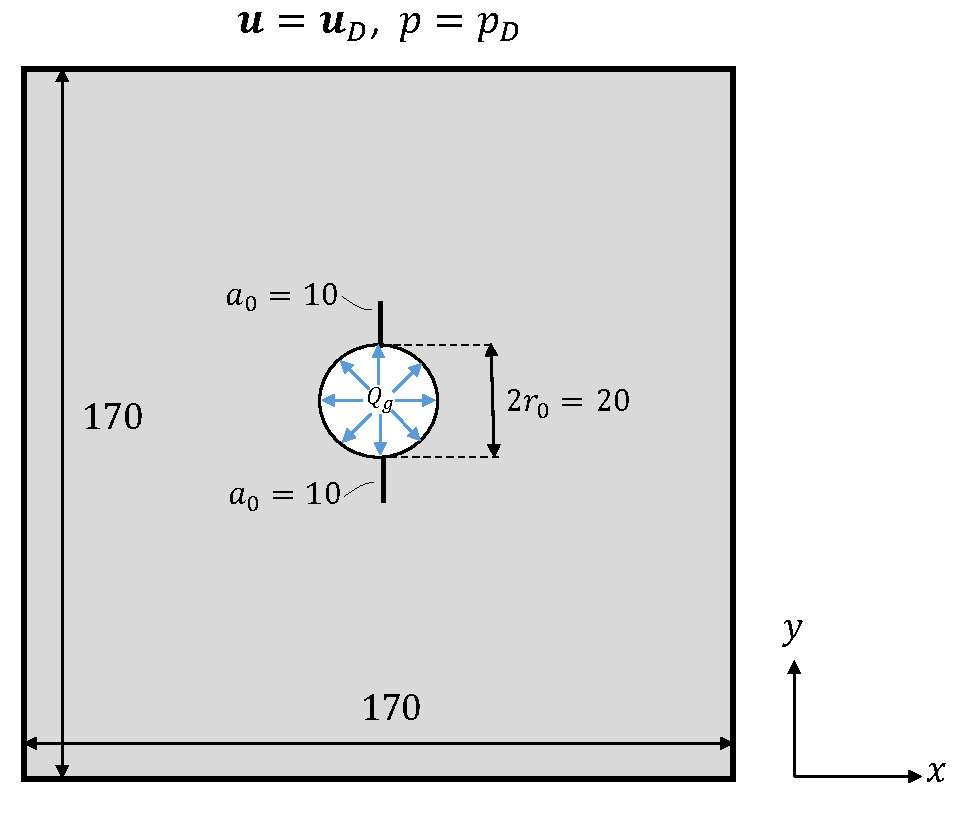
\includegraphics[width=0.8\textwidth]{GasFrackingModel2}
	\caption{Schematic of a cracked square plate (unit: mm) with pressurized CO$_2$ flow.}
	\label{Fig:Gas_geometry}
\end{figure}

As in Figure \ref{Fig:Gas_geometry}, there exist two preexisting fractures representing the perforations. We set $d=1$ for both fractures and set the Dirichlet boundary condition $d=0$ on the external boundary. The fluid is continuously injected into the central borehole with diameter $2r_0=20$ mm, until after the fractures propagate. Note that in this problem, the isothermal condition is adopted so that CO$_2$ is in the supercritical phase ($T=45^{\circ}$C).
%\todo[inline]{We have to mention our computation domain would be $\Omega-$ the borehole. It  is worth to mention the boundary of borehole is denoted by $\gamma_B$\\Vahid: Now that we have added Figure \ref{Fig:compute_domain}, there is no need for further explanations here.}


For the sake of simplicity, the \emph{in situ} stress is imposed on the boundary by means of its ``equivalent'' prescribed displacement. More precisely, the displacement of the same specimen with no crack under the same \emph{in situ} stress is first computed, then used as the Dirichlet boundary condition for the problem at hand. On the external boundary, we set $p=p_D$ where $p_D=0$. Moreover, $\Gamma_P=\Gamma_D$ in this example.

%\todo[inline]{YS: What is the purpose of putting a reference \cite{wang2018influence} ALONE in the title of Table \ref{Tab:Gas_input}? More words are needed, like ``according to.''\\Vahid: Changed.}

\begin{table}[htbp]
    \centering
    \caption{Default parameter values for the example. These values are taken from \cite{wang2018influence} except $g_c$, which is from \eqref{Eq:choice_ell}.}

    \begin{tabular}{l c c c}
    \hline 
         Parameters & symbol & unit& value \\
    \hline 
         Young's modulus & $E$ &MPa&  6 $\times 10^{3}$\\
         Poisson's ratio & $\nu$ &$-$&  0.34\\
         Critical energy release rate & $g_c$ &MPa$\cdot$mm&  0.306\\
         %Regularization length scale & $\ell$ &$-$&  1.6$\times 10^{-4}$\\
         Biot coefficient & $\alpha$ &$-$&  0.85\\
         Porosity & $\phi$ &$-$&  0.01\\
         Initial permeability & $k_0$ &mm$^2$&  1$\times 10^{-12}$\\
         Dynamic viscosity of  {CO}$_2$ & $\mu$ & MPa$\cdot$s& 4.04$\times 10^{-11}$\\
         %Bulk modulus of fluid & $k_f$ &$KN/mm^2$&  0.625$ \times 10^{3}$\\
        % Bulk modulus of rock & $k_s$ &$KN/mm^2$&  10$ \times 10^{3}$\\
         Initial pressure & $p_0$ &MPa&  0.1\\
         Rock's tensile strength & $\sigma_T$ &MPa&  11\\
         %Maximum principal stress & $\sigma_1$ &MPa&  1\\
         %Minimum  principal stress & $\sigma_3$ &MPa&  1\\

    \hline     
    \end{tabular}
    \label{Tab:Gas_input}
\end{table}

%\begin{figure}[htbp]
%\centering %
%\subfloat[]{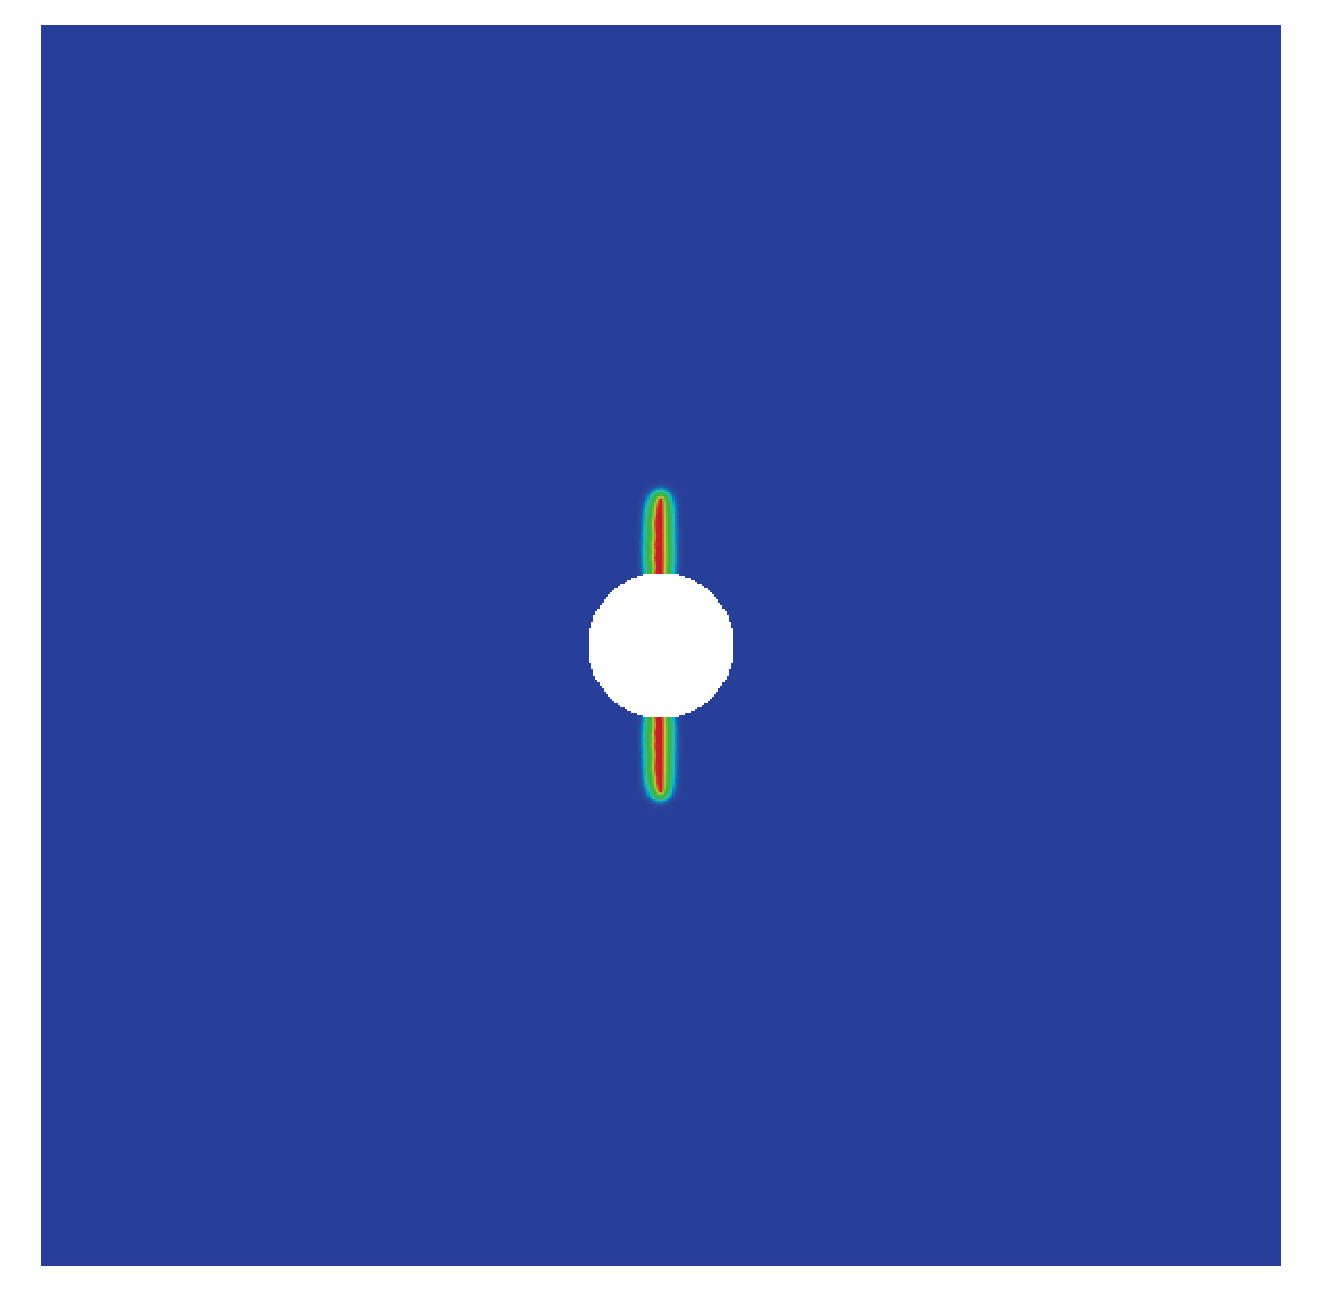
\includegraphics[width=60mm]{alpha_50.eps}\label{Fig:Gas_d_i}}
%\subfloat[]{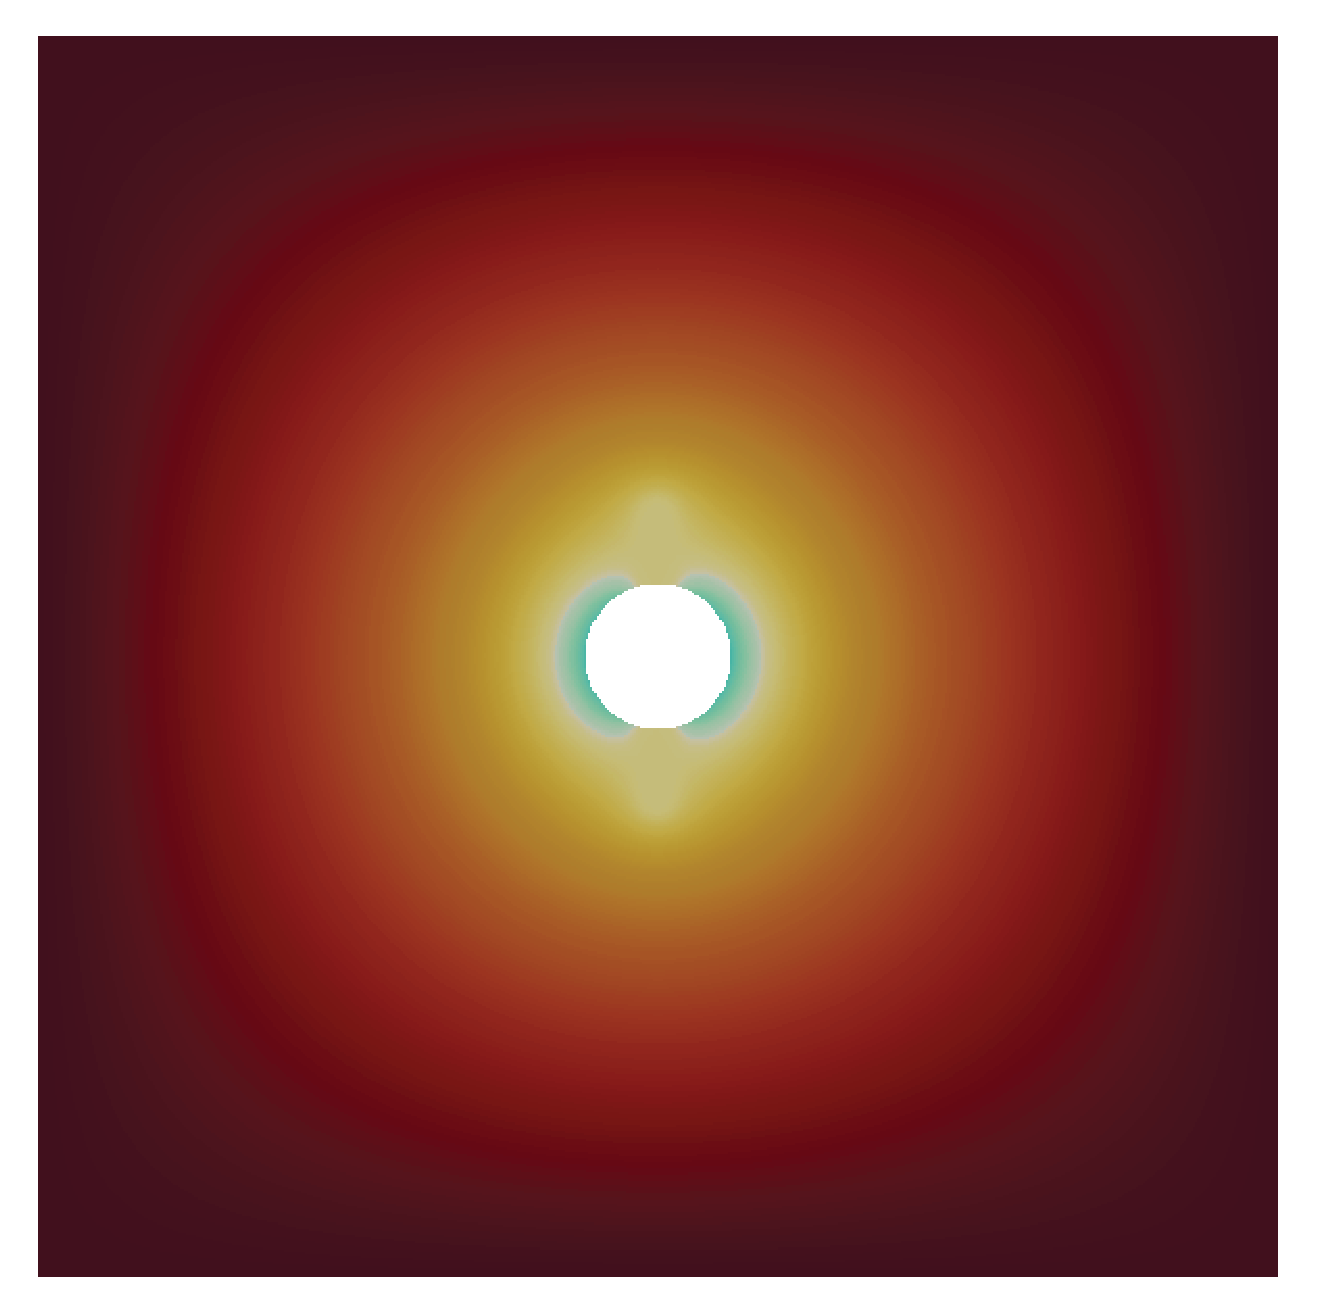
\includegraphics[width=60mm]{pressure_50.eps}\label{Fig:Gas_p_i}}\\
%\subfloat[]{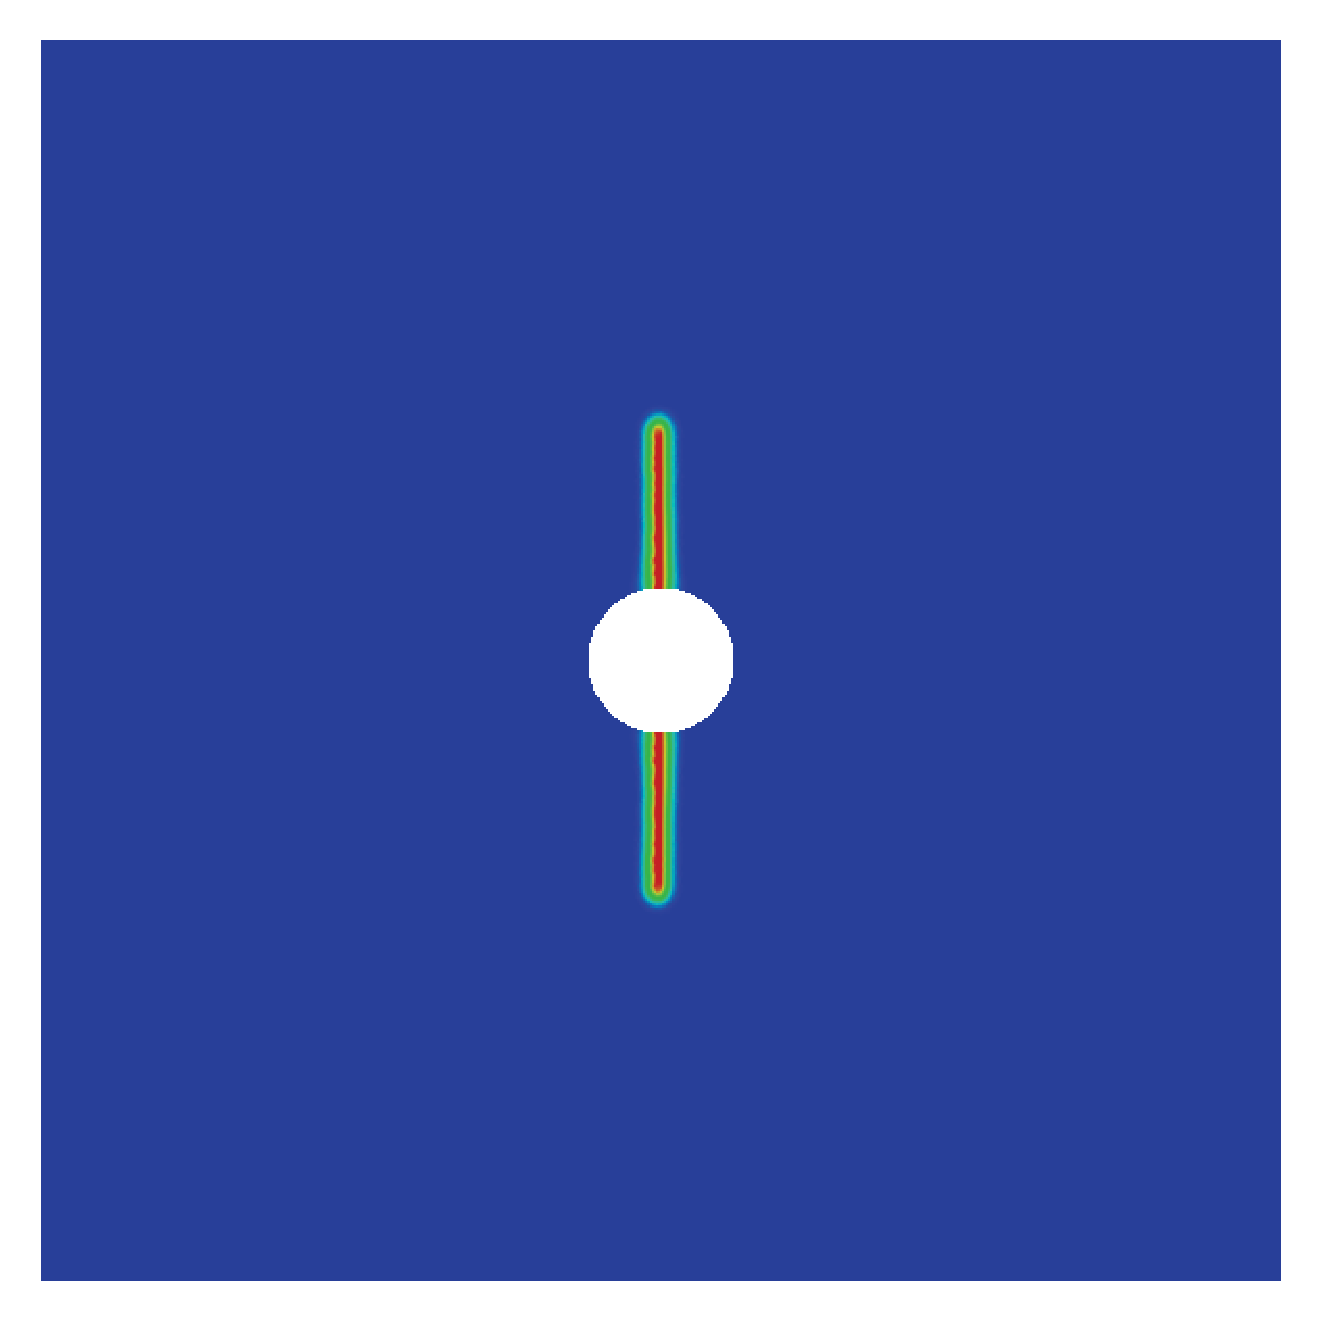
\includegraphics[width=60mm]{alpha_75.eps}\label{Fig:Gas_d_ii}}
%\subfloat[]{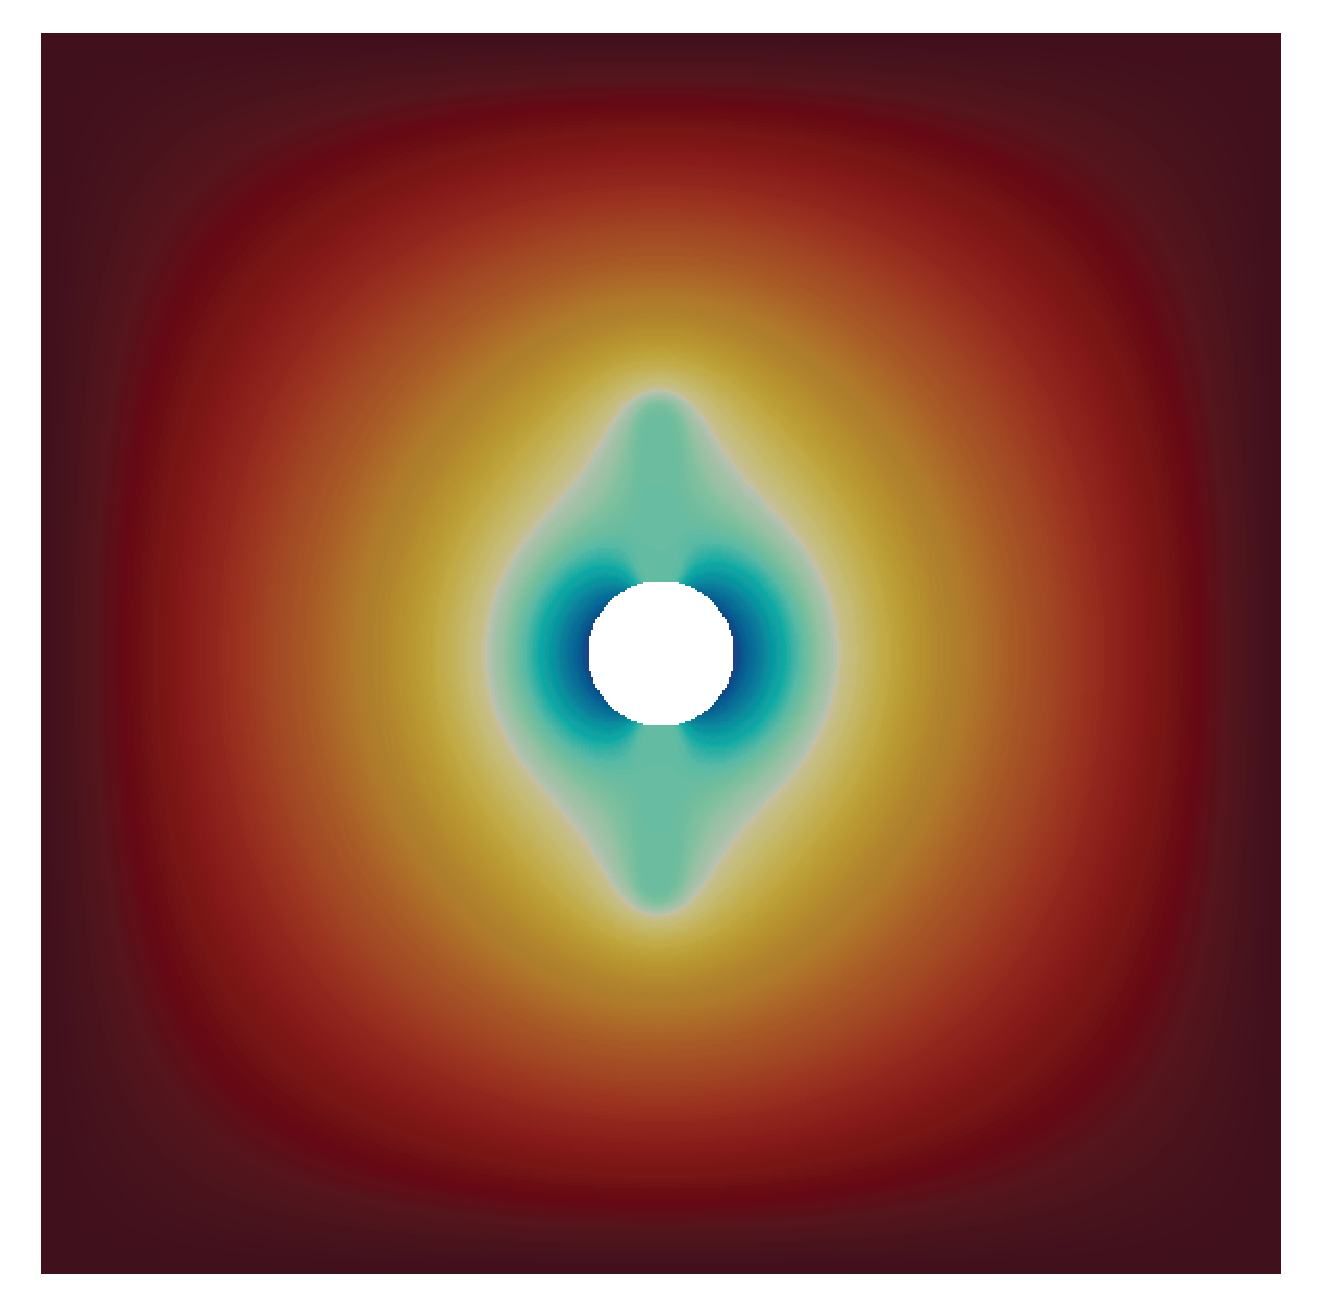
\includegraphics[width=60mm]{pressure_75.eps}\label{Fig:Gas_p_ii}}\\
%\subfloat[]{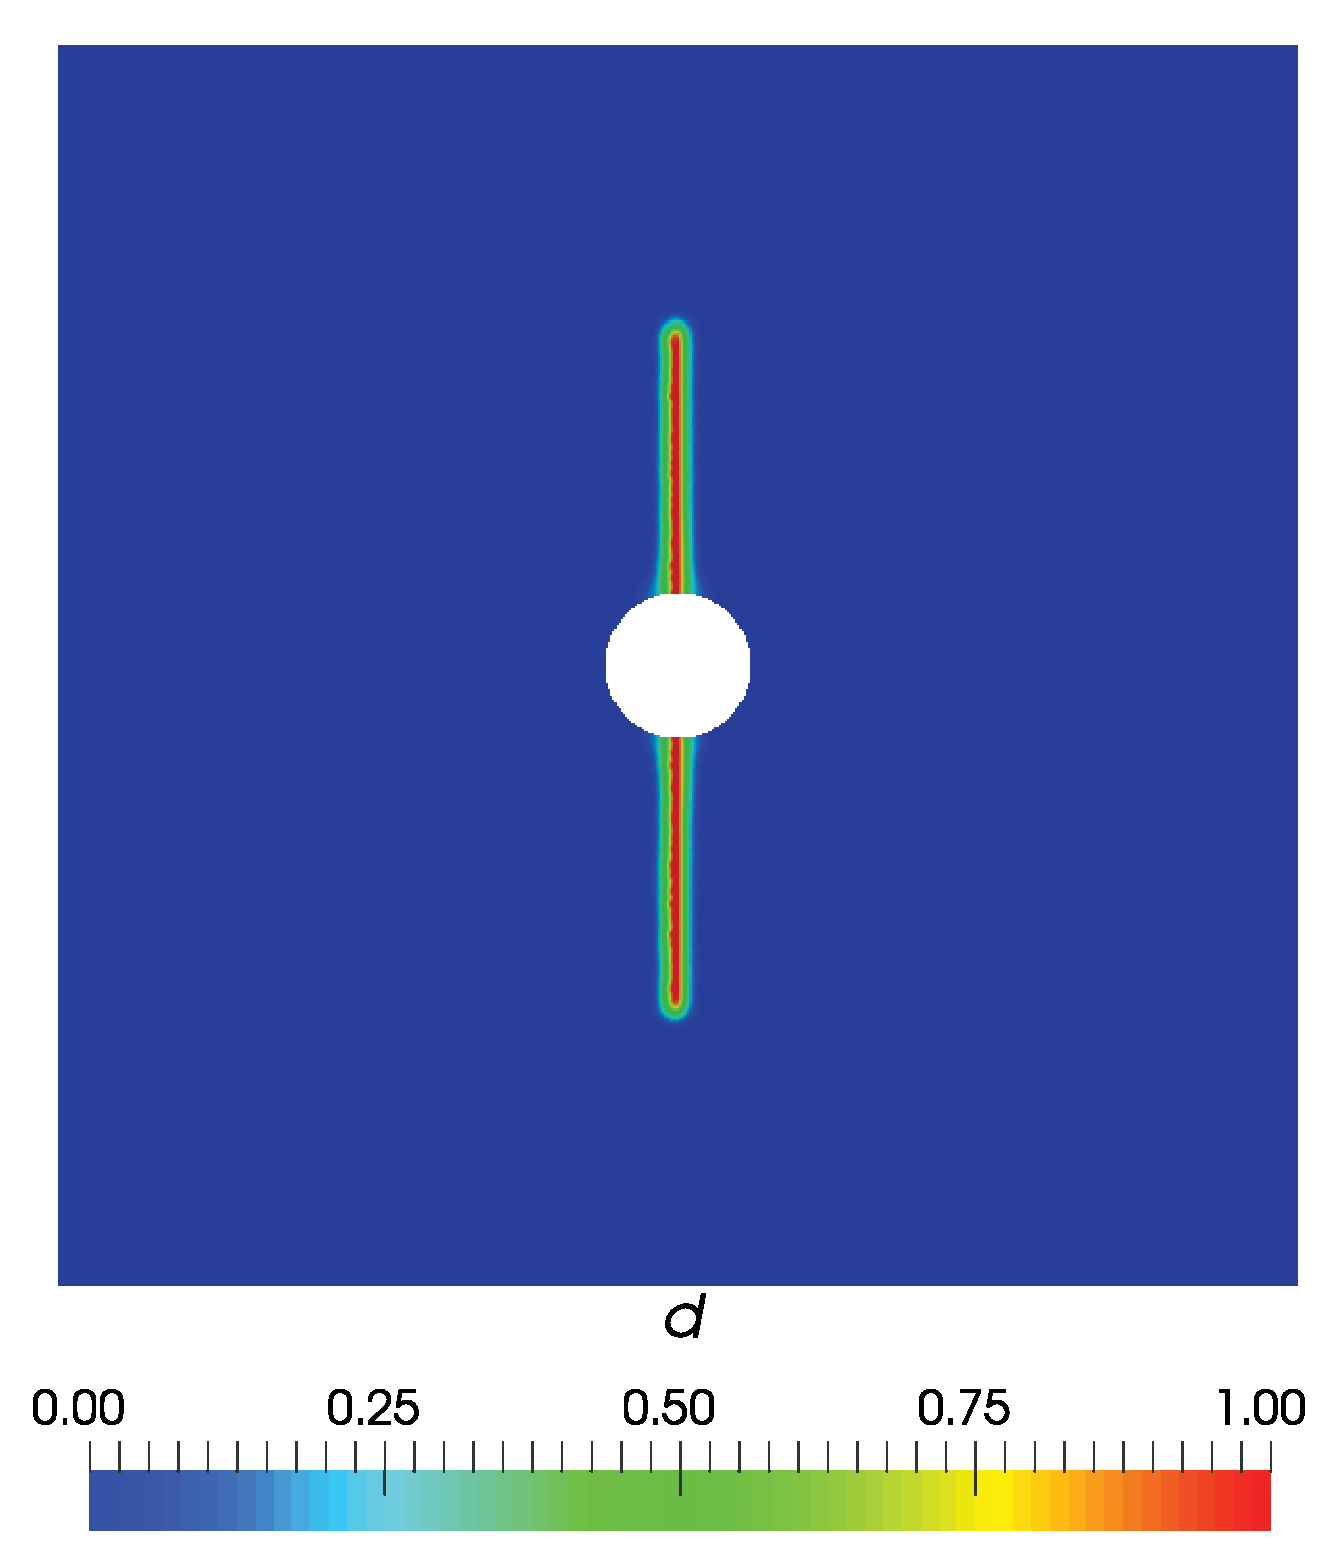
\includegraphics[width=60mm]{alpha_100.eps}\label{Fig:Gas_d_iii}}
%\subfloat[]{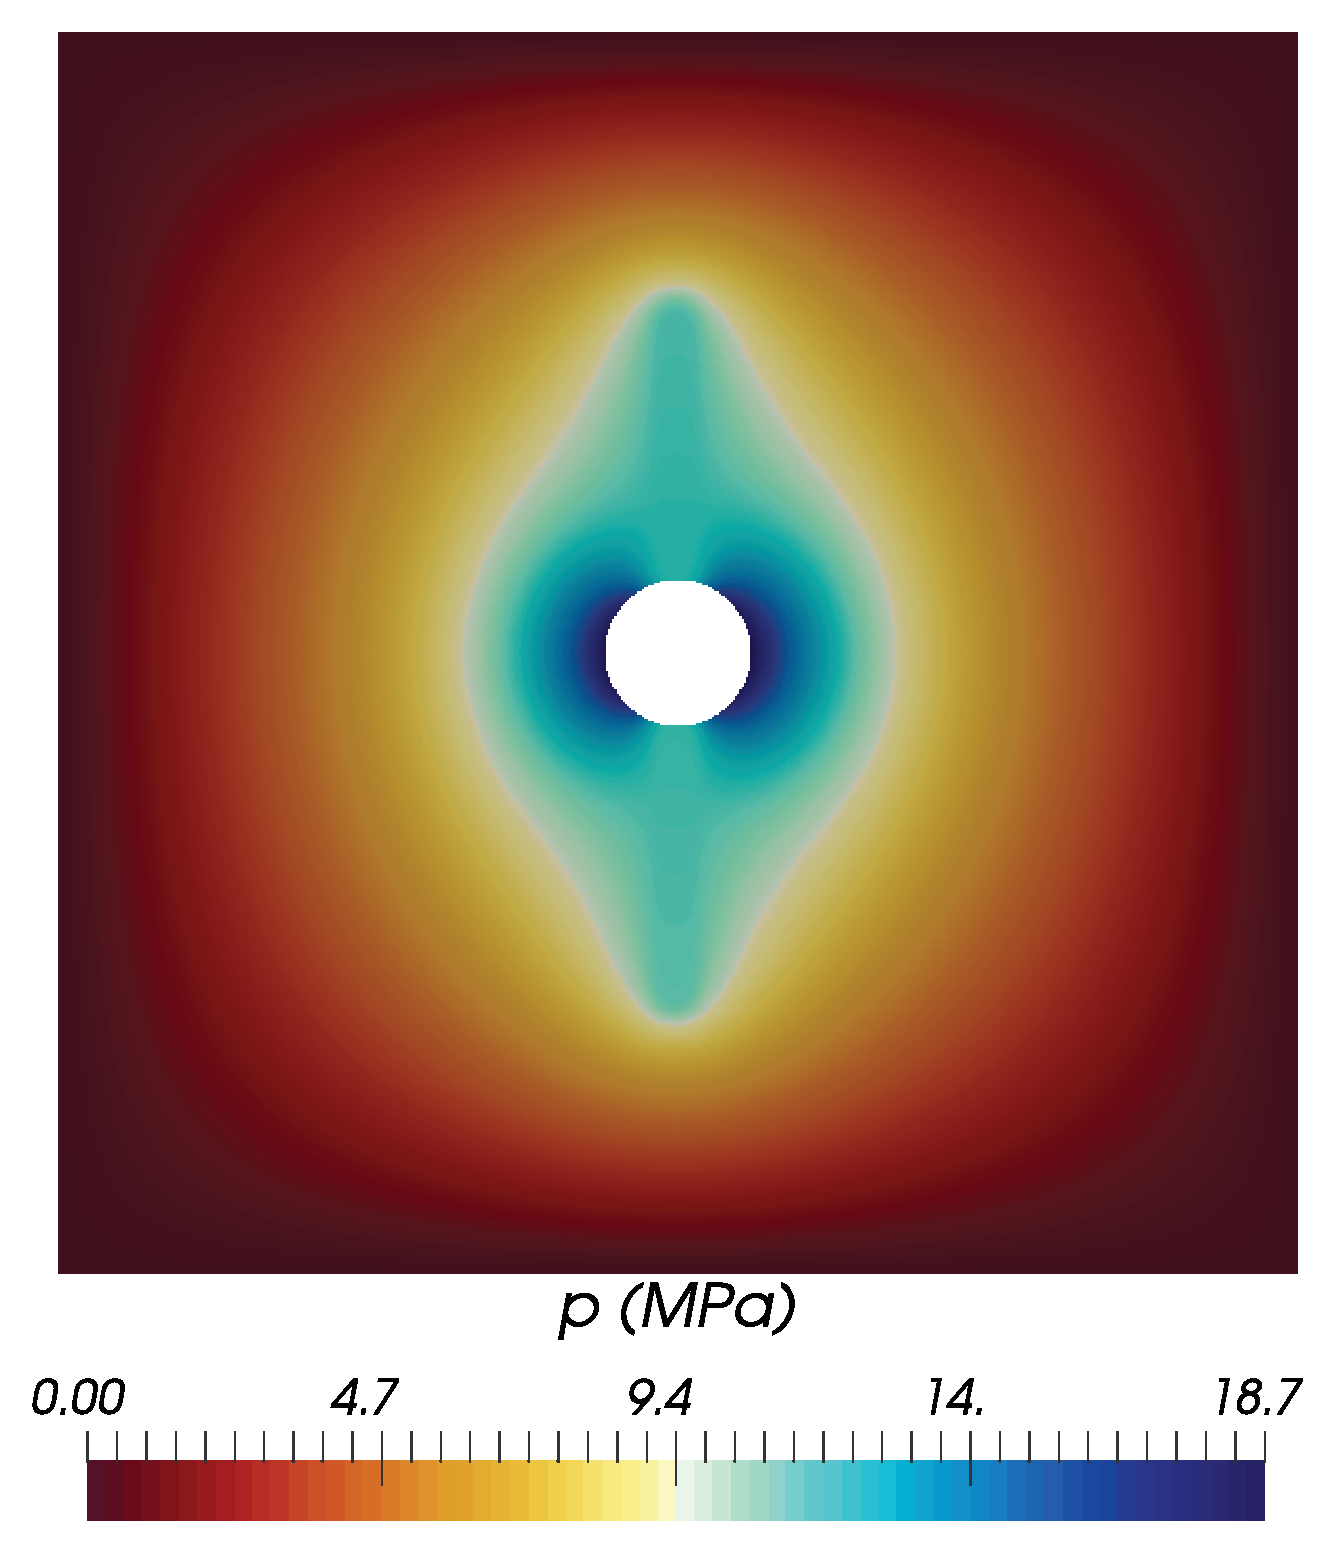
\includegraphics[width=60mm]{pressure_100.eps}\label{Fig:Gas_p_iii}}
%\caption{Left: Phase field diagram at different stages (\ref{Fig:Gas_d_i}) $t=0.5t_f$, (\ref{Fig:Gas_d_ii}) $t=0.75t_f$, and (\ref{Fig:Gas_d_iii}) $t=t_f$). Right: Pressure profile at (\ref{Fig:Gas_p_i}) $t=0.5t_f$, (\ref{Fig:Gas_p_ii}) $t=0.75t_f$, and (\ref{Fig:Gas_p_iii}) $t=t_f$.}
%\label{Fig:Gas_snapshots}
%\end{figure}




\begin{figure}[htbp]
\centering %
\subfloat[]{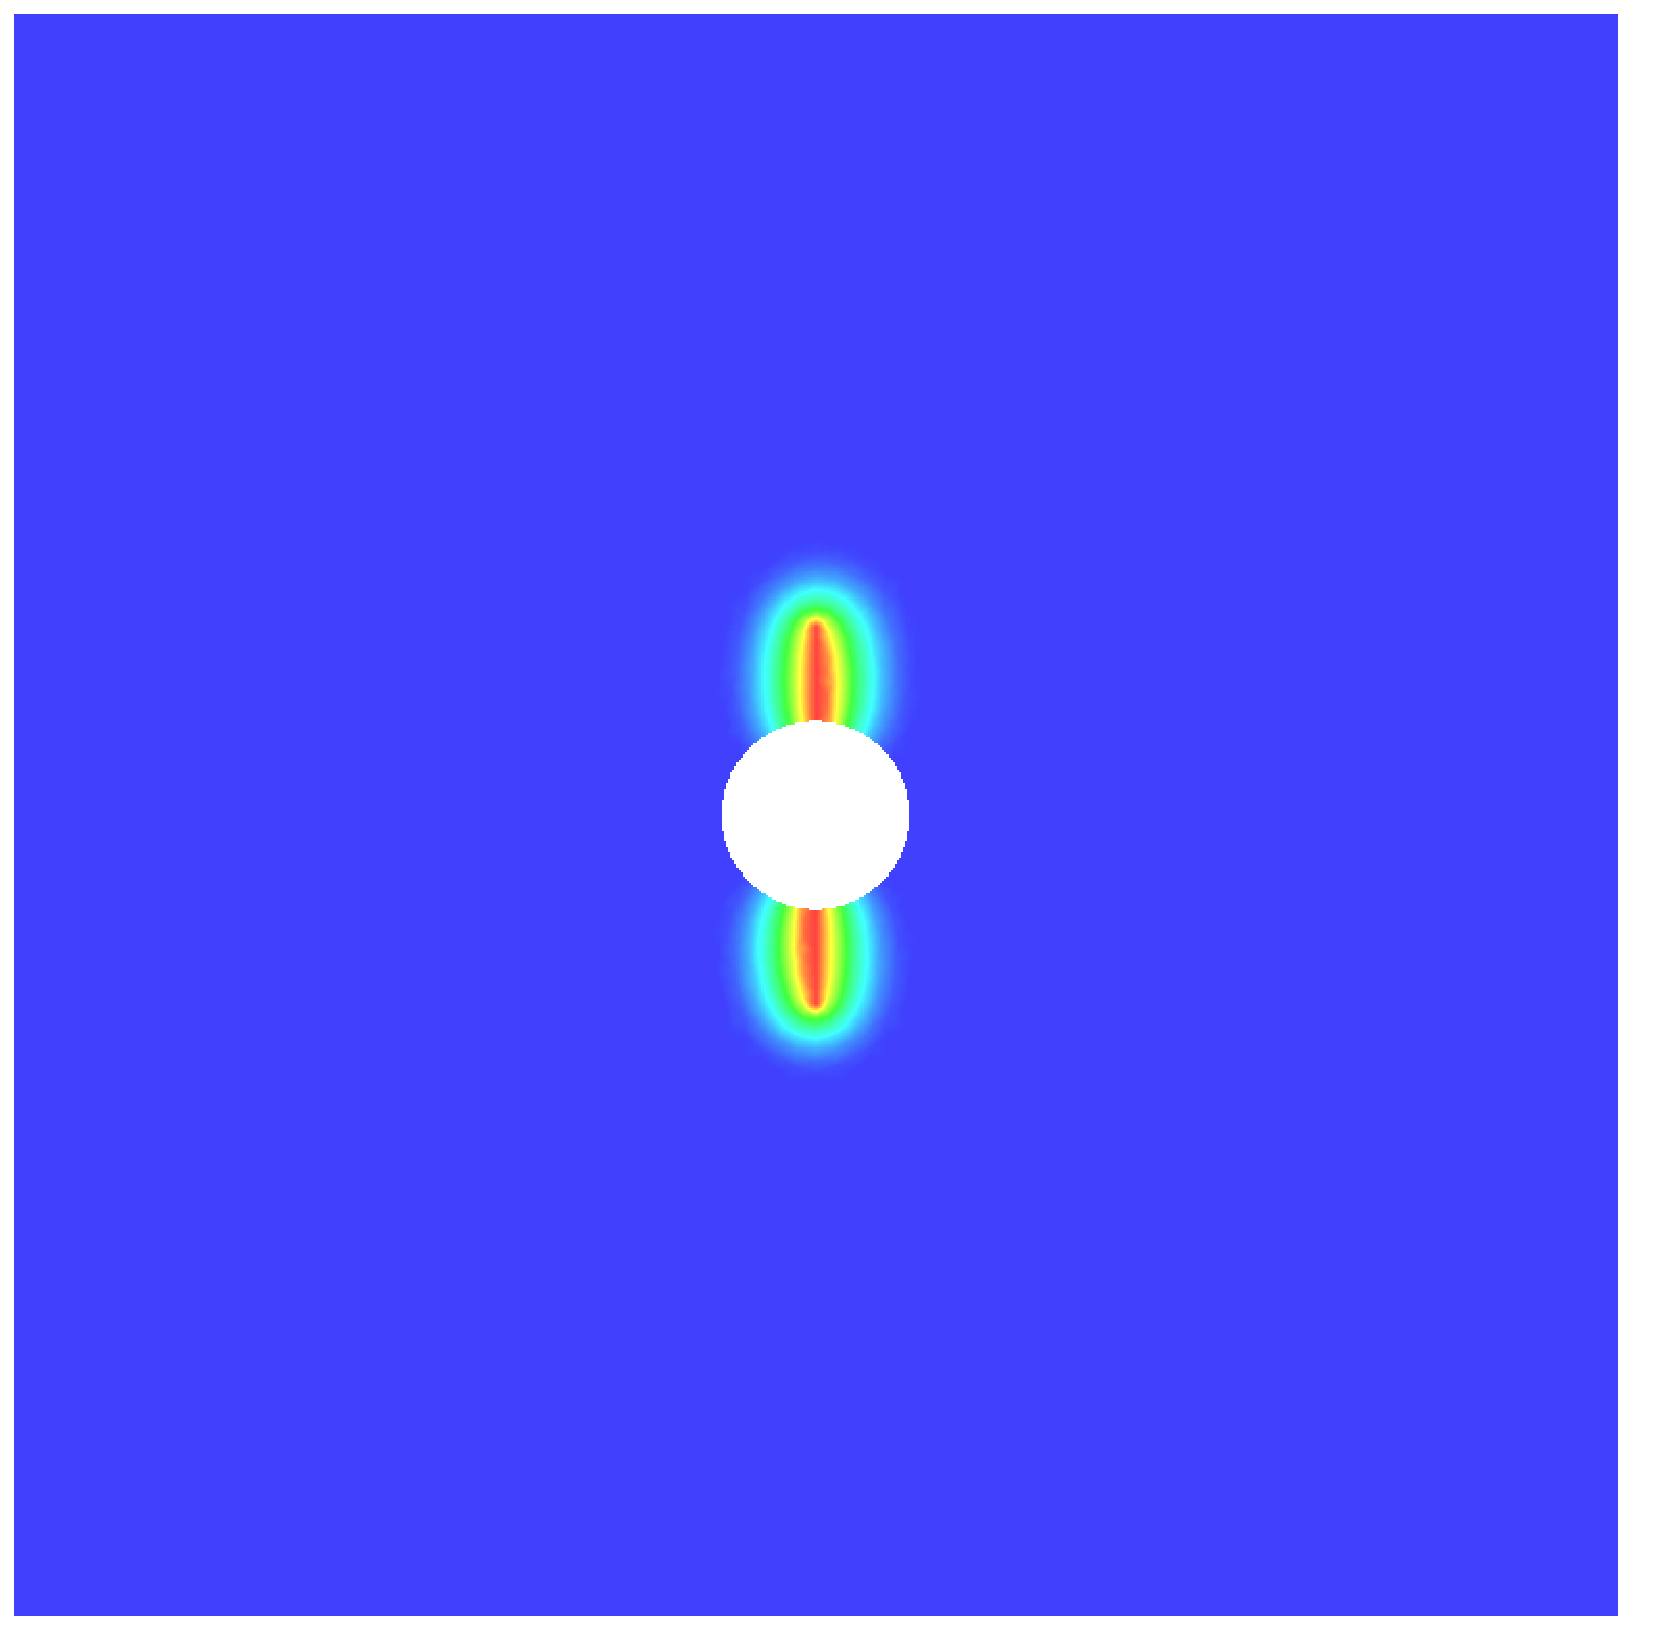
\includegraphics[width=60mm]{alpha25}\label{Fig:Gas_d_i}}
\subfloat[]{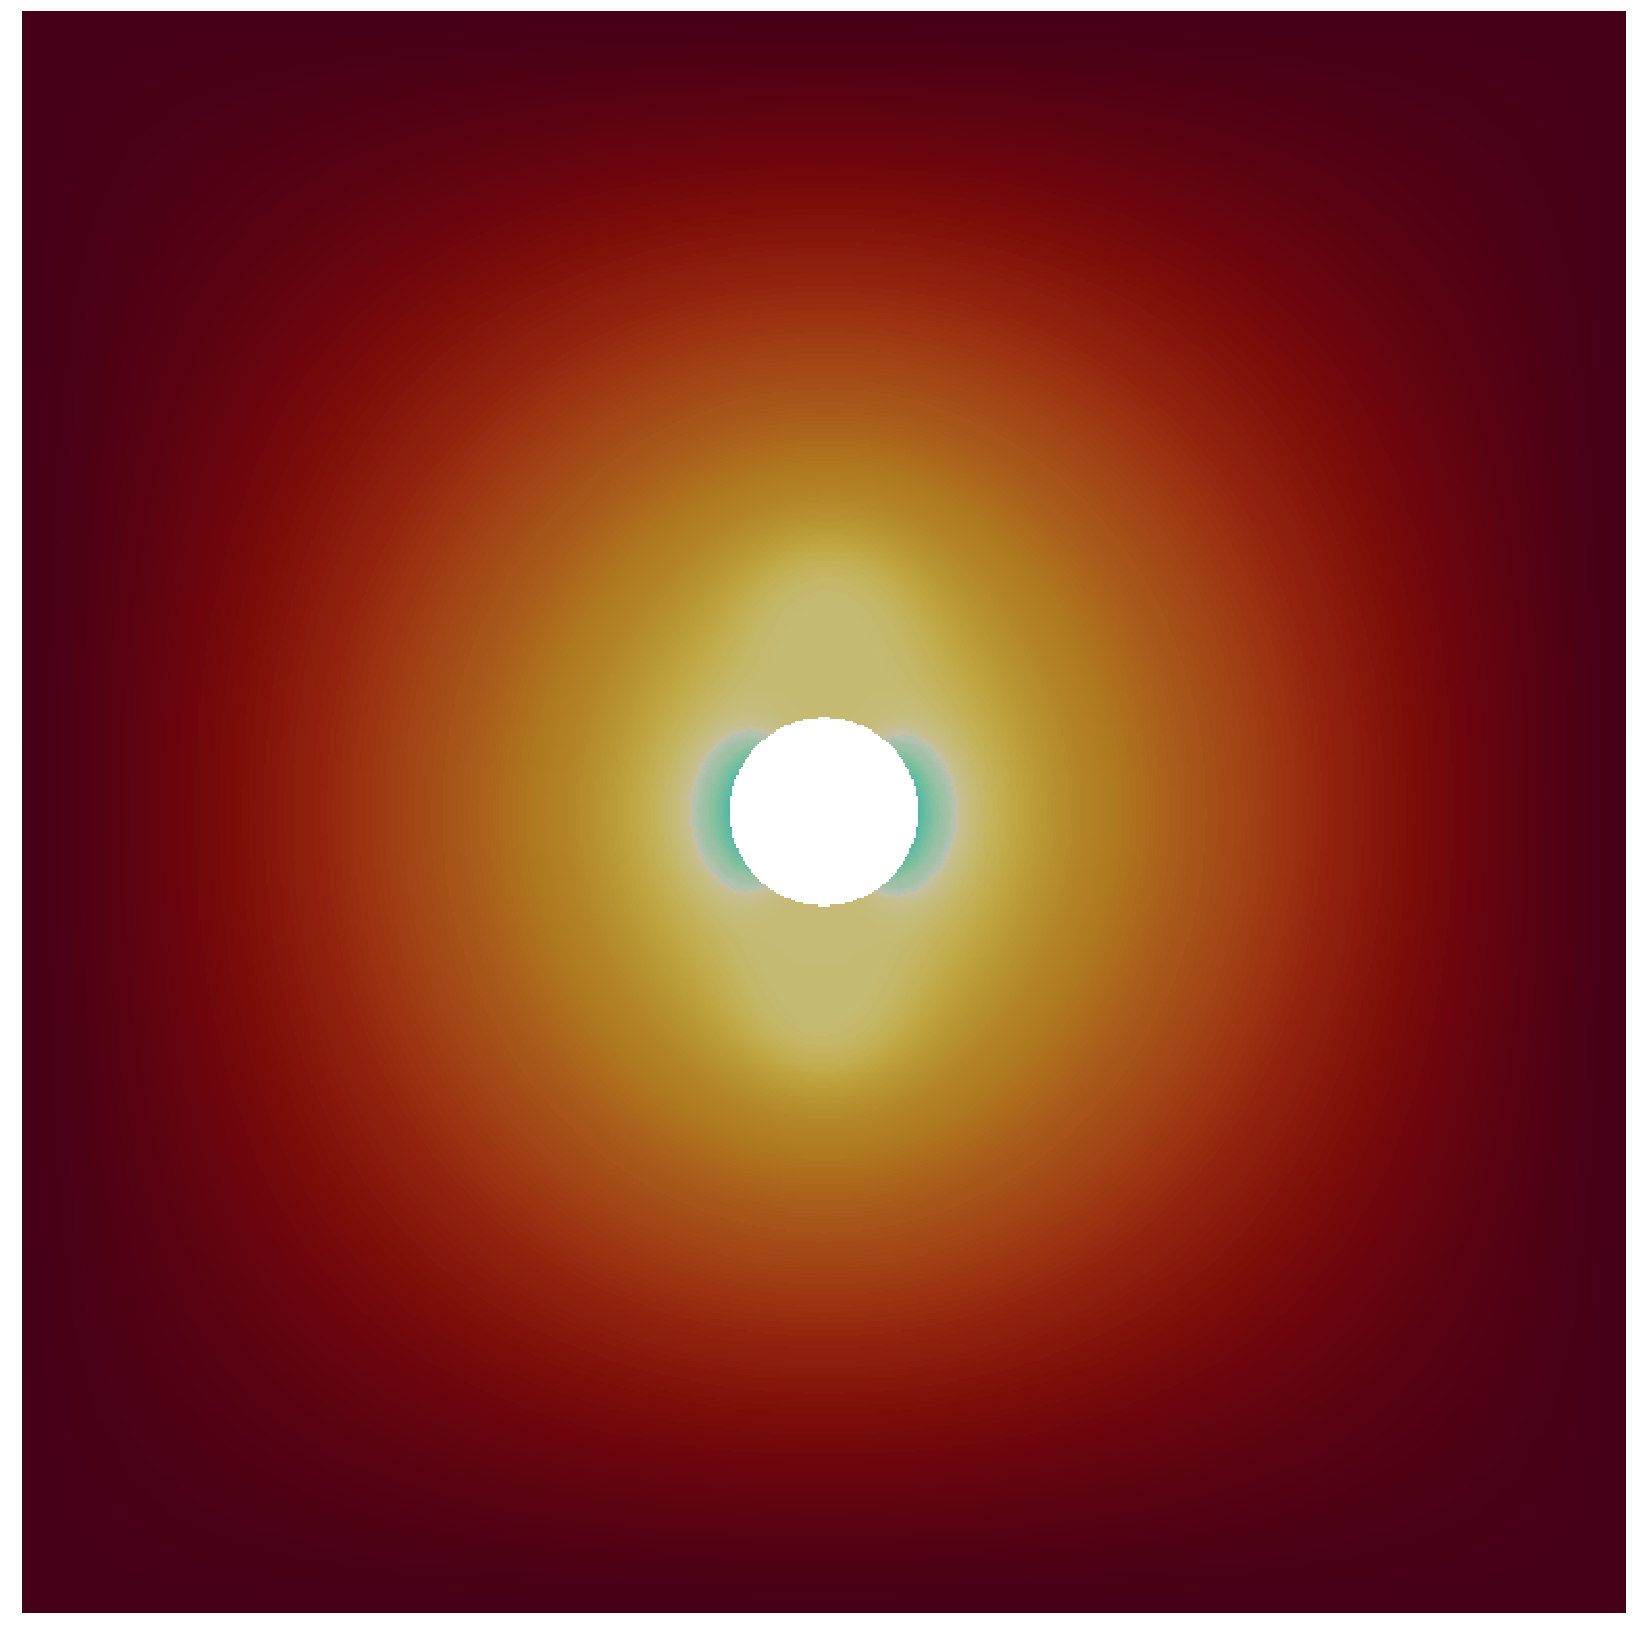
\includegraphics[width=60mm]{pressure25}\label{Fig:Gas_p_i}}\\
\subfloat[]{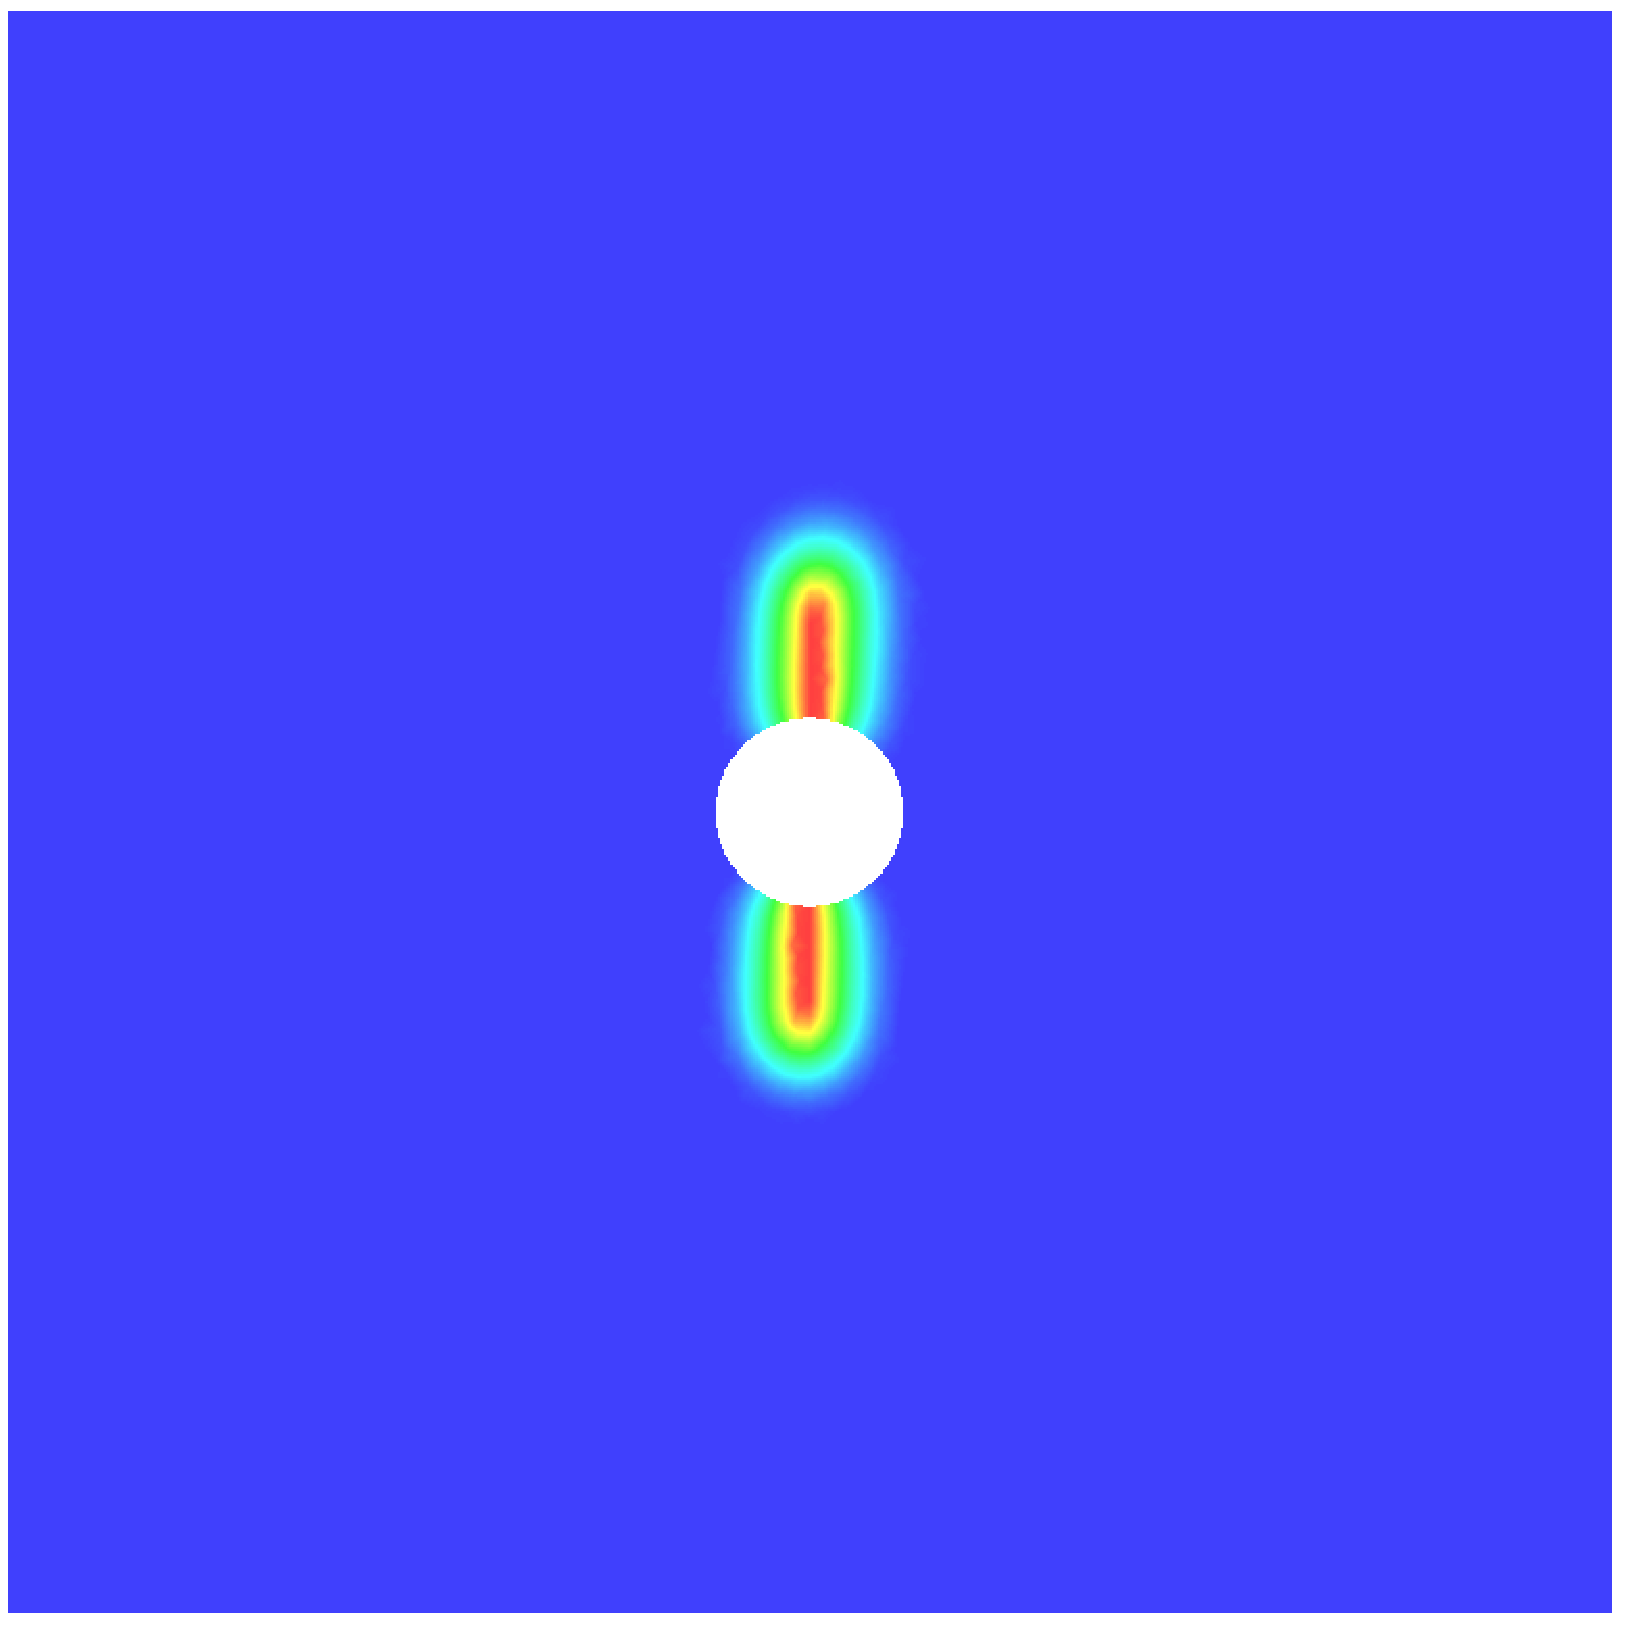
\includegraphics[width=60mm]{alpha37}\label{Fig:Gas_d_ii}}
\subfloat[]{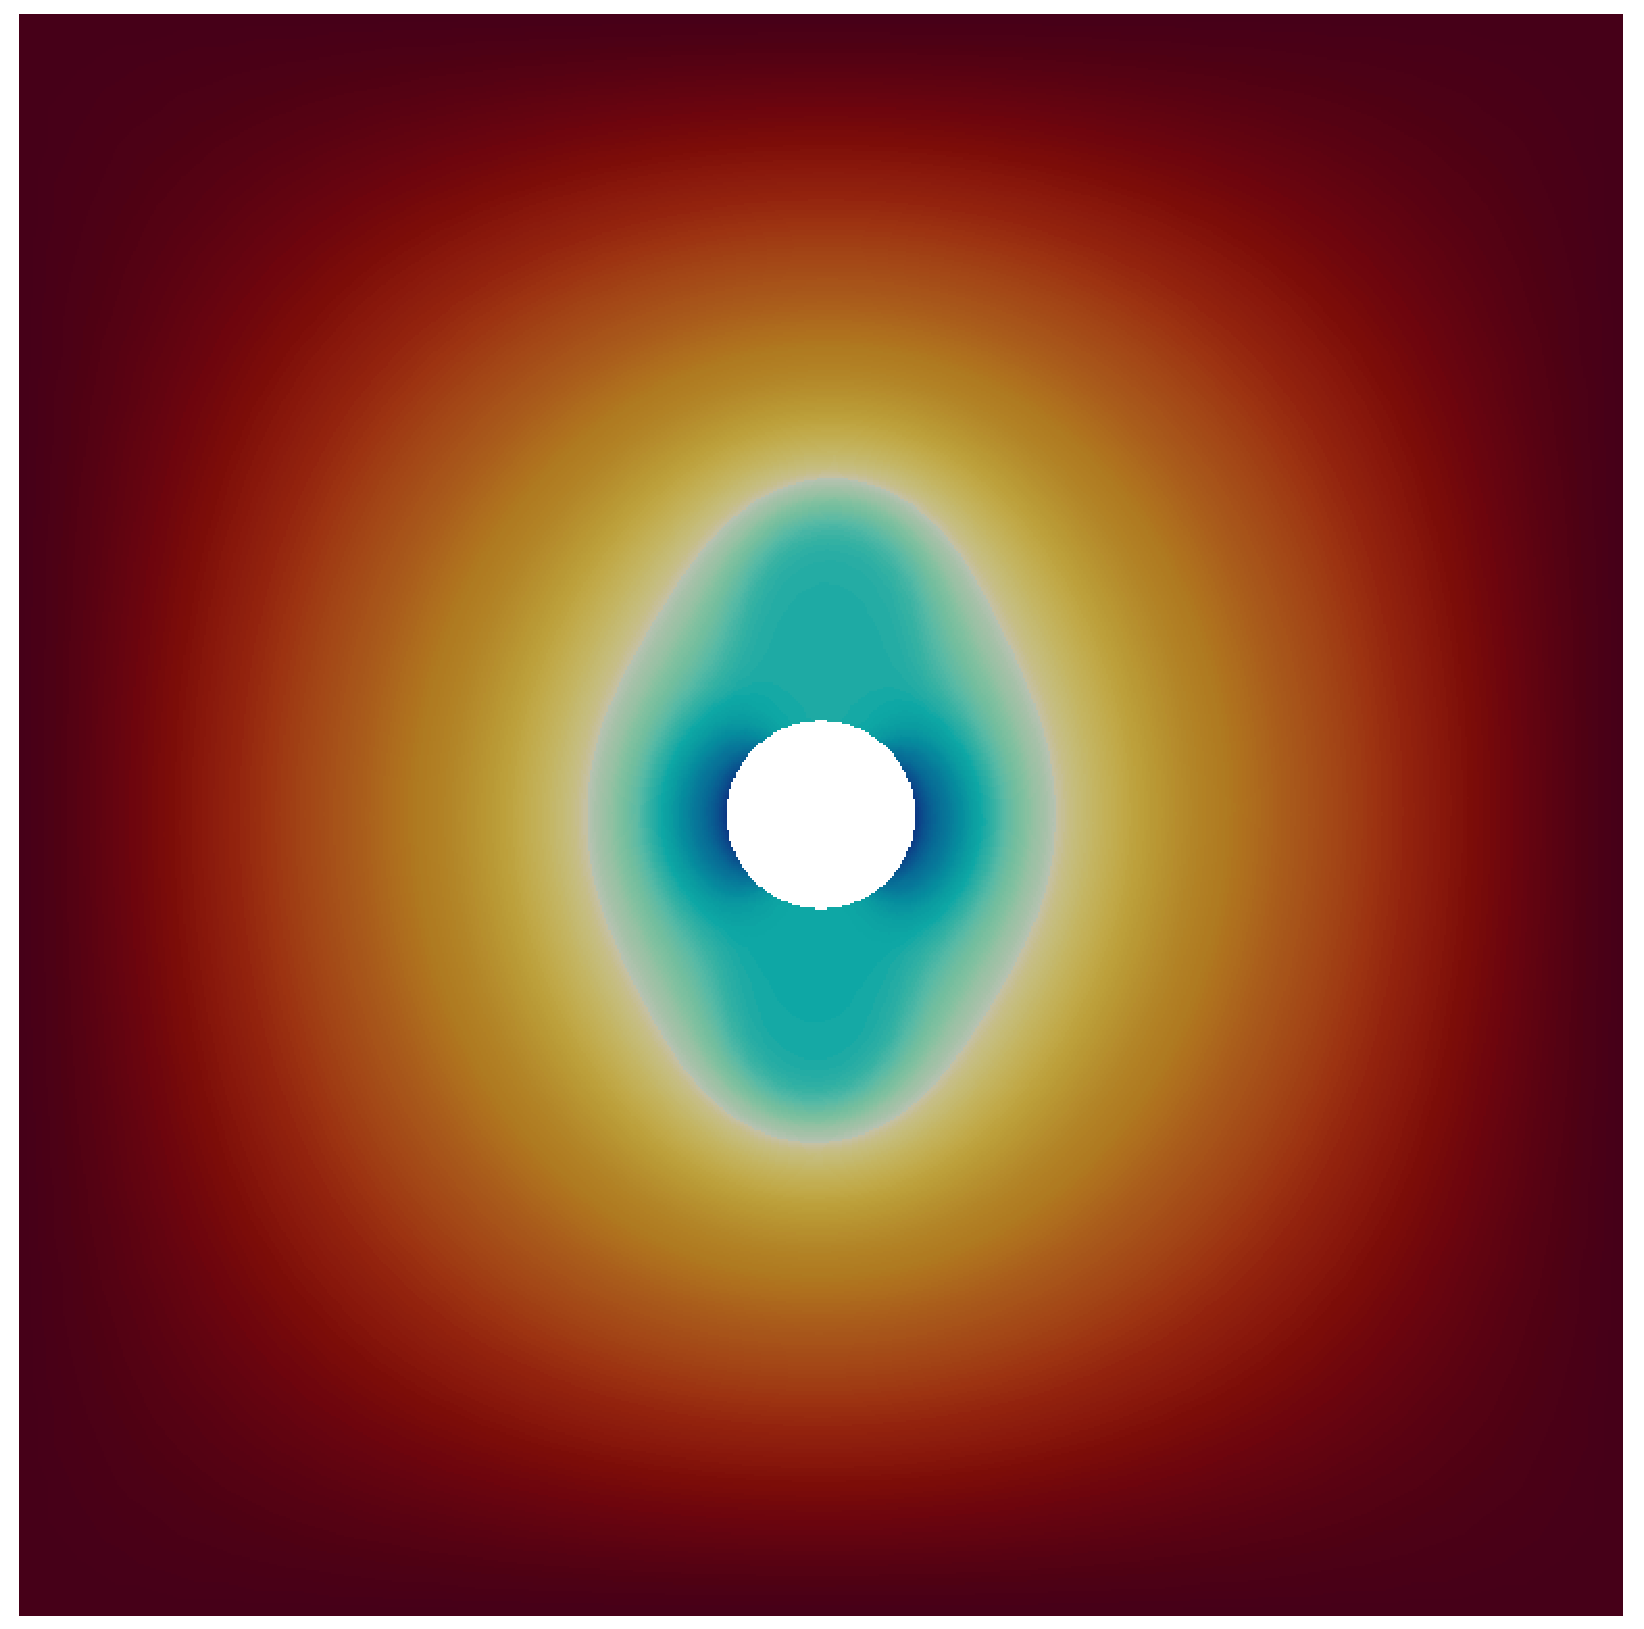
\includegraphics[width=60mm]{pressure37}\label{Fig:Gas_p_ii}}\\
\subfloat[]{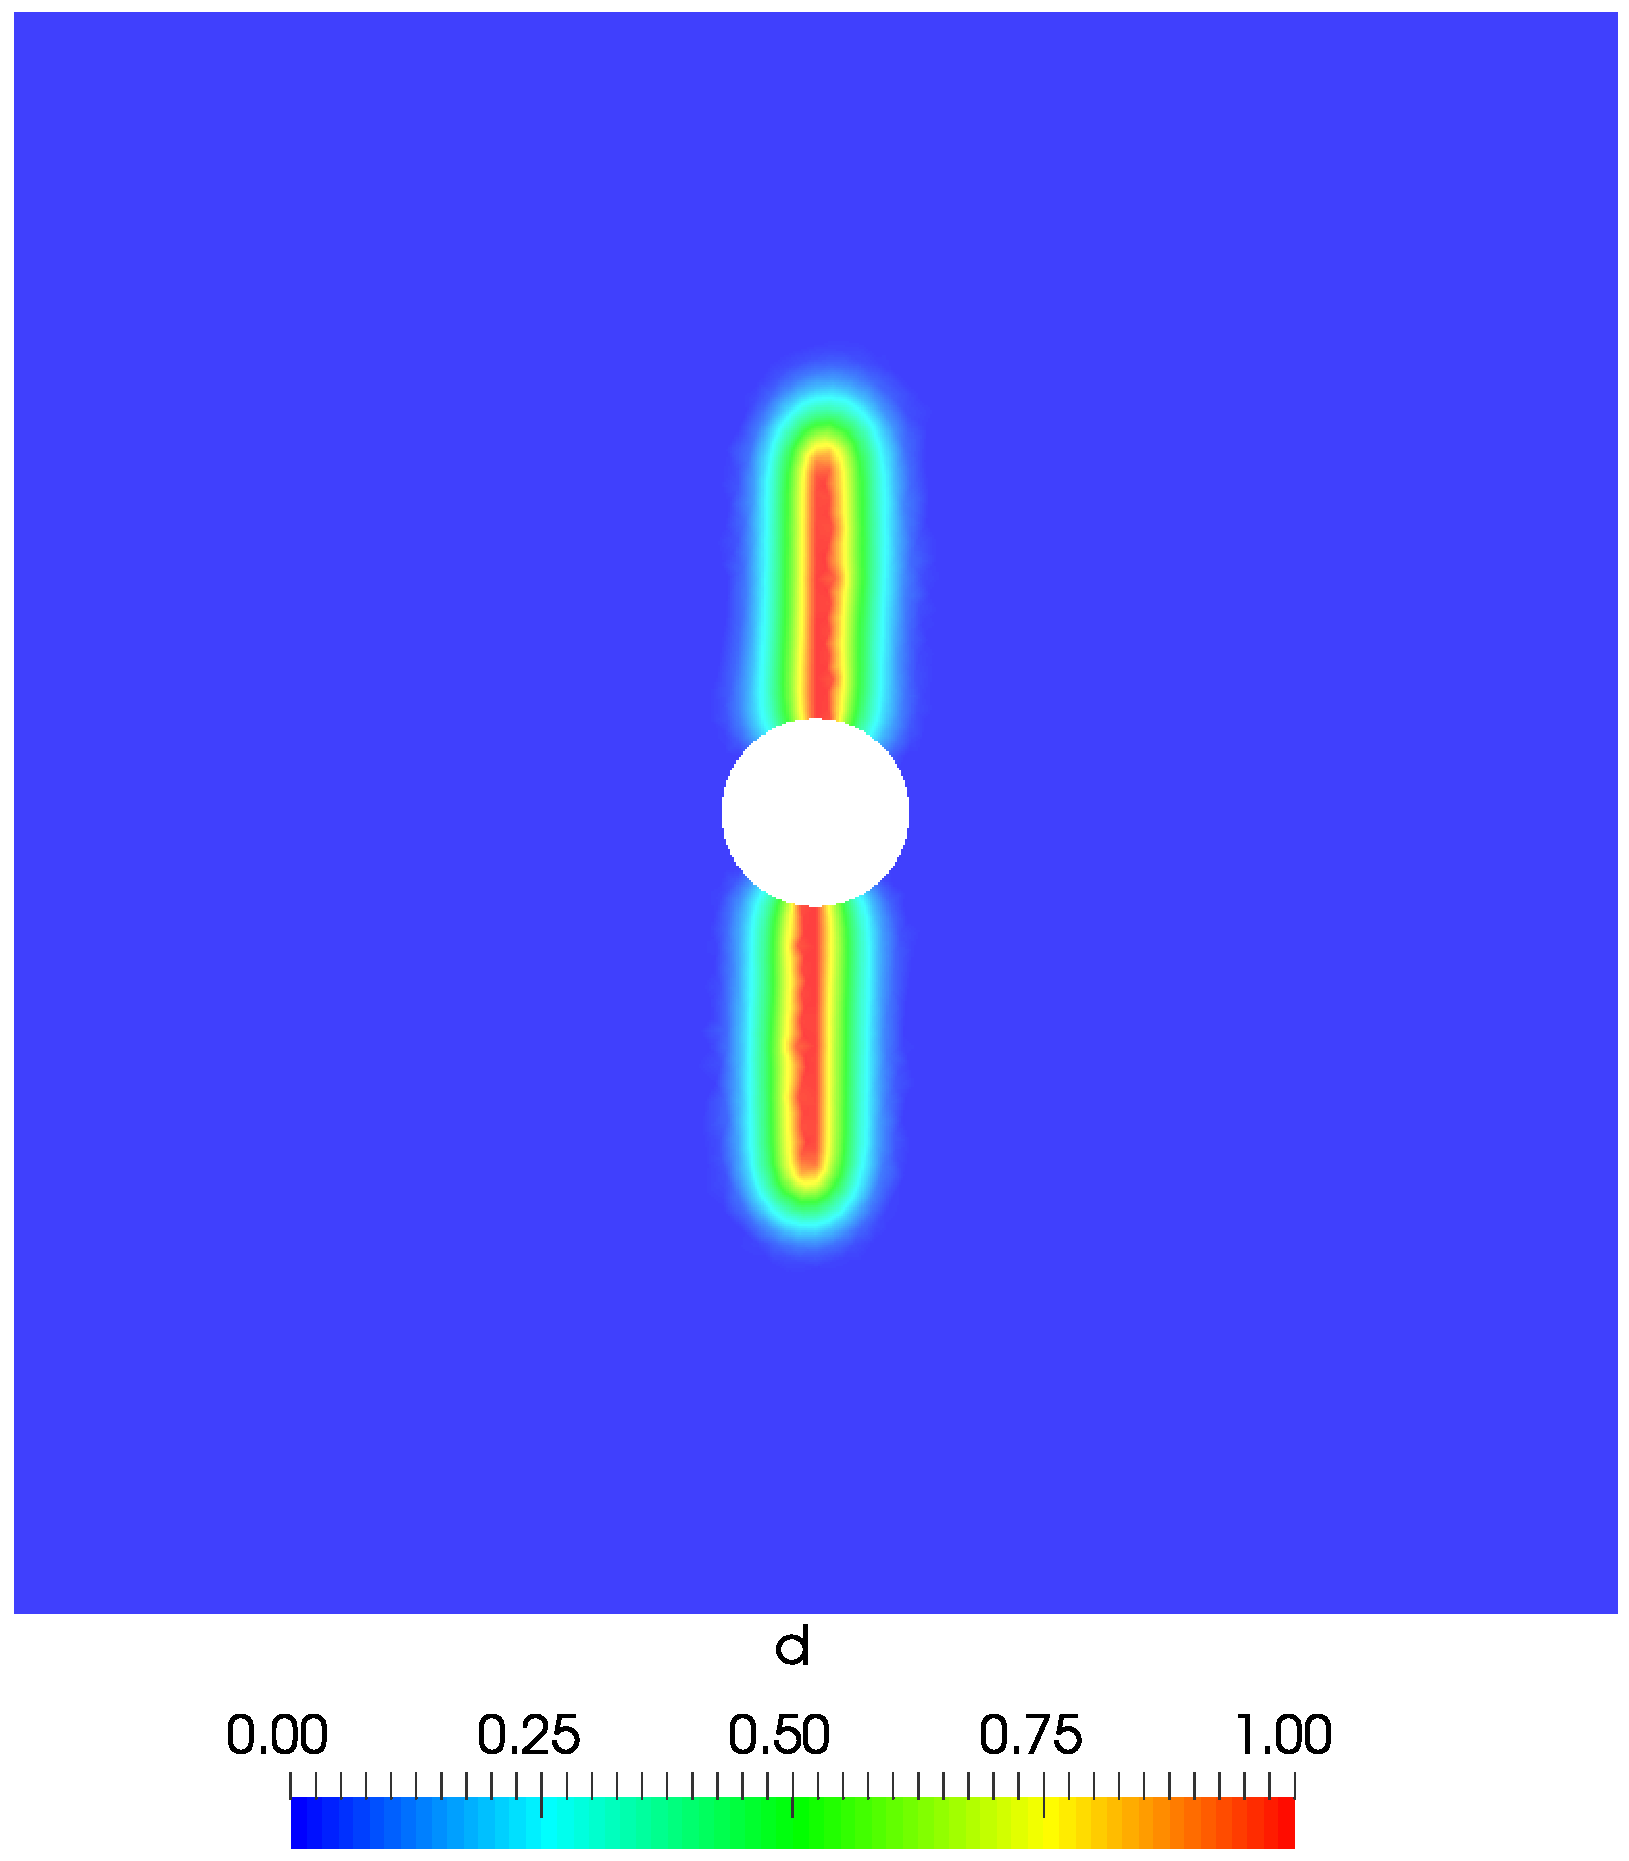
\includegraphics[width=60mm]{alpha49}\label{Fig:Gas_d_iii}}
\subfloat[]{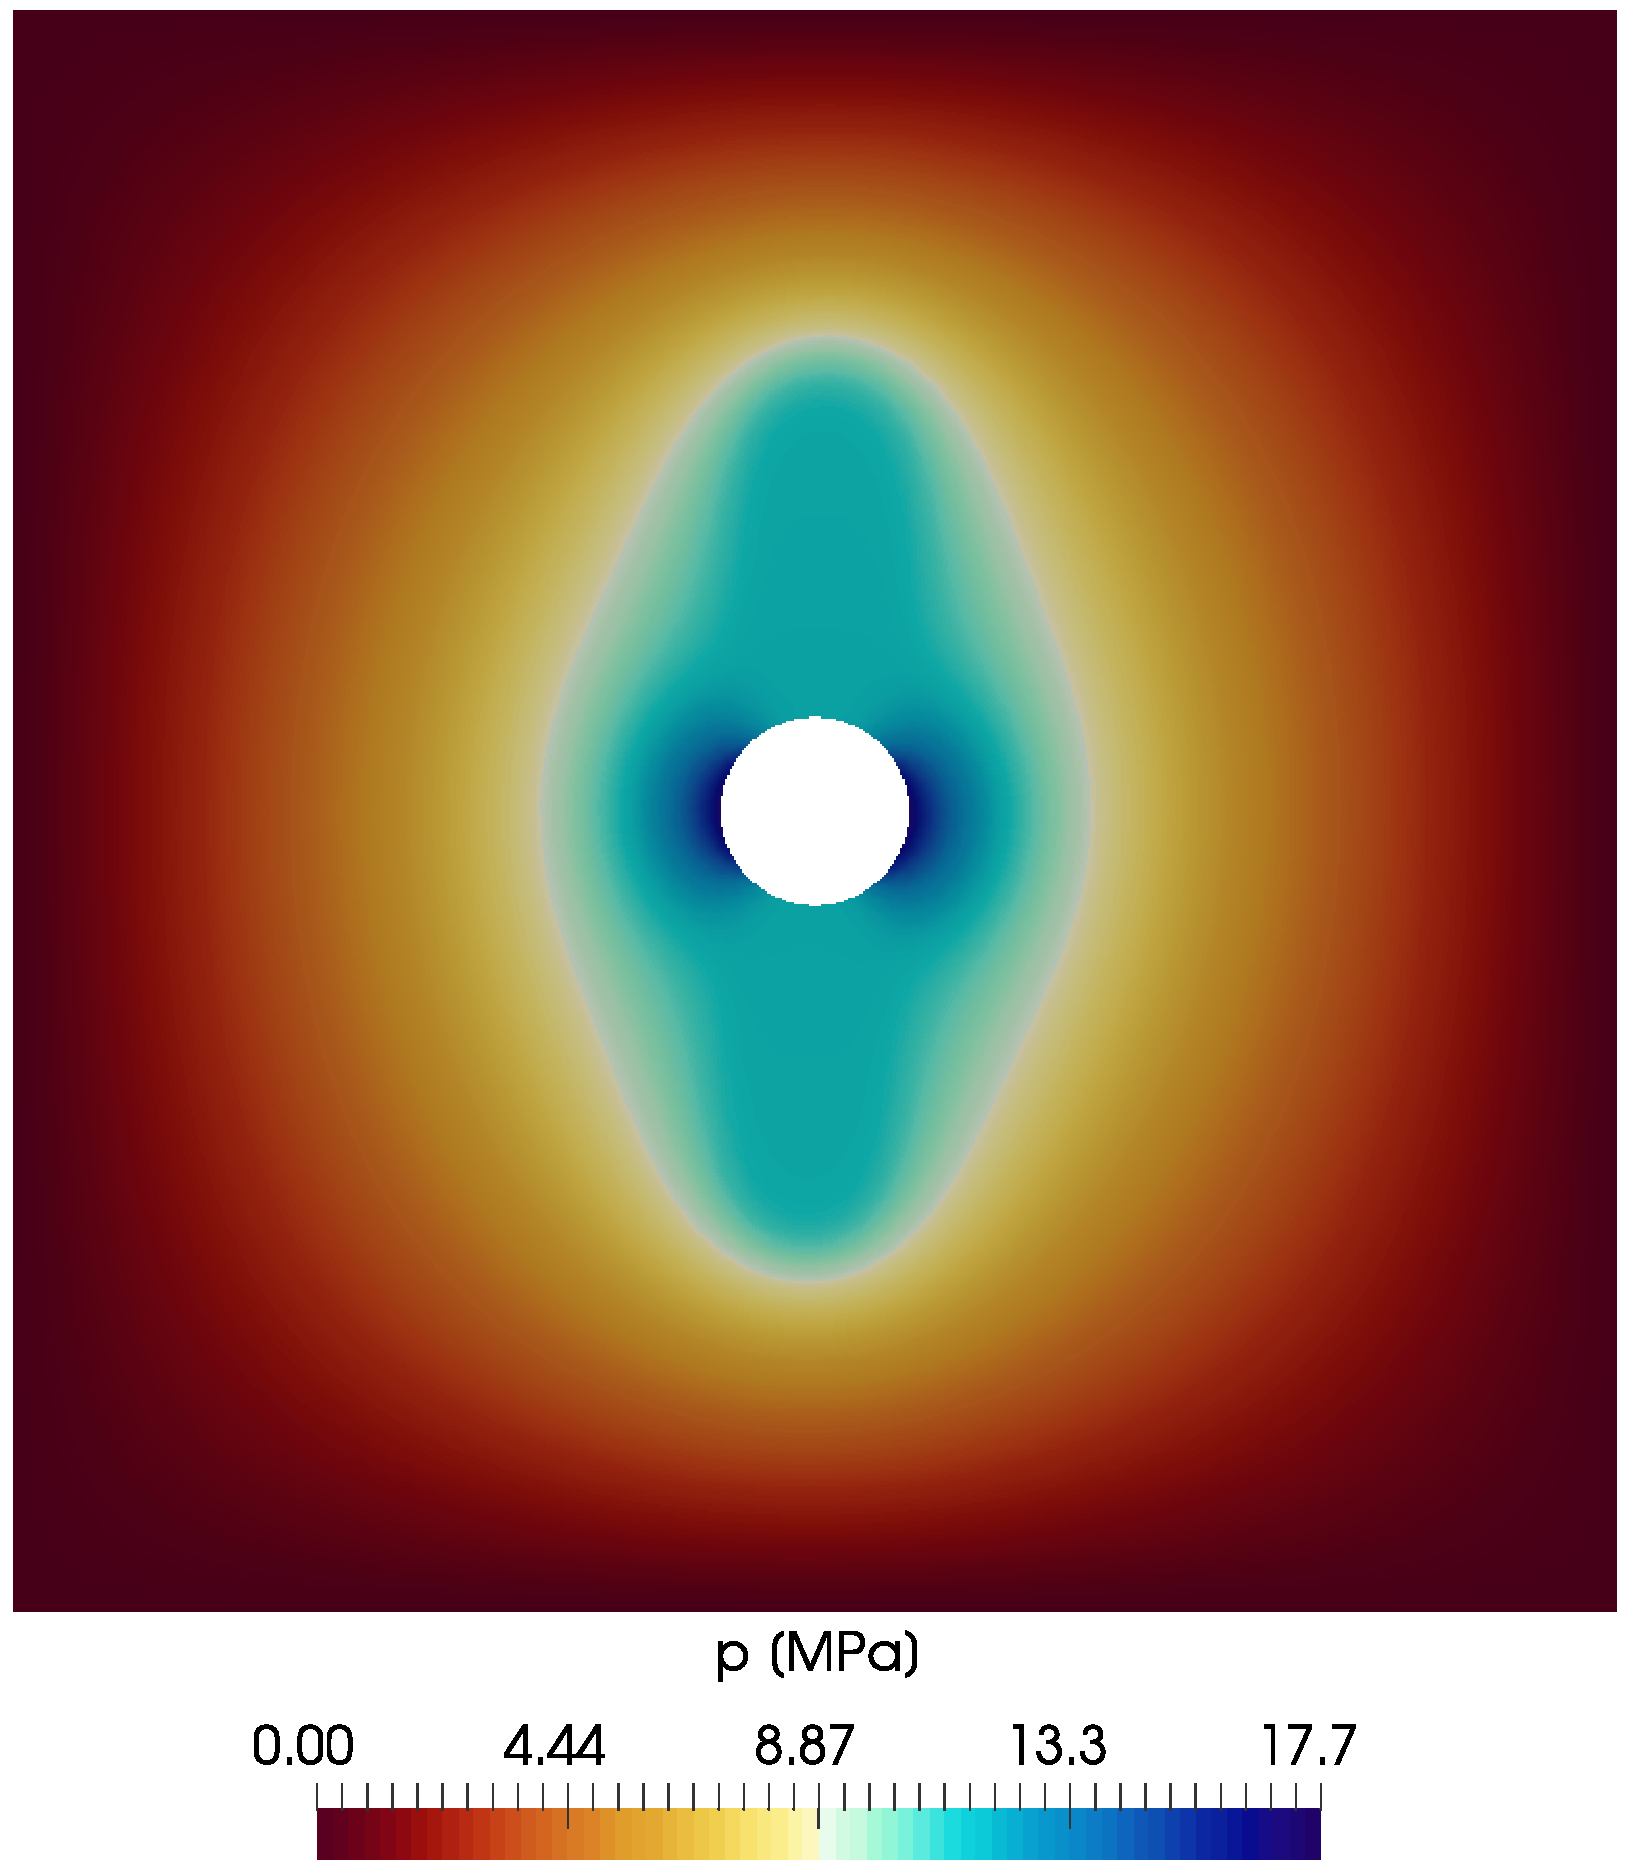
\includegraphics[width=60mm]{pressure49}\label{Fig:Gas_p_iii}}
\caption{Left: Phase field diagram at different stages (\ref{Fig:Gas_d_i}) $t=0.5t_f$, (\ref{Fig:Gas_d_ii}) $t=0.74t_f$, and (\ref{Fig:Gas_d_iii}) $t=t_f$). Right: Pressure profile at (\ref{Fig:Gas_p_i}) $t=0.5t_f$, (\ref{Fig:Gas_p_ii}) $t=0.74t_f$, and (\ref{Fig:Gas_p_iii}) $t=t_f$.}
\label{Fig:Gas_snapshots}
\end{figure}



%\todo[inline]{YS: The natural order is to first give OUR prediction of the breakdown pressure, then compare it with classical solutions.\\
%Vahid: The order is changed. See below.}

\begin{figure}
    \centering
    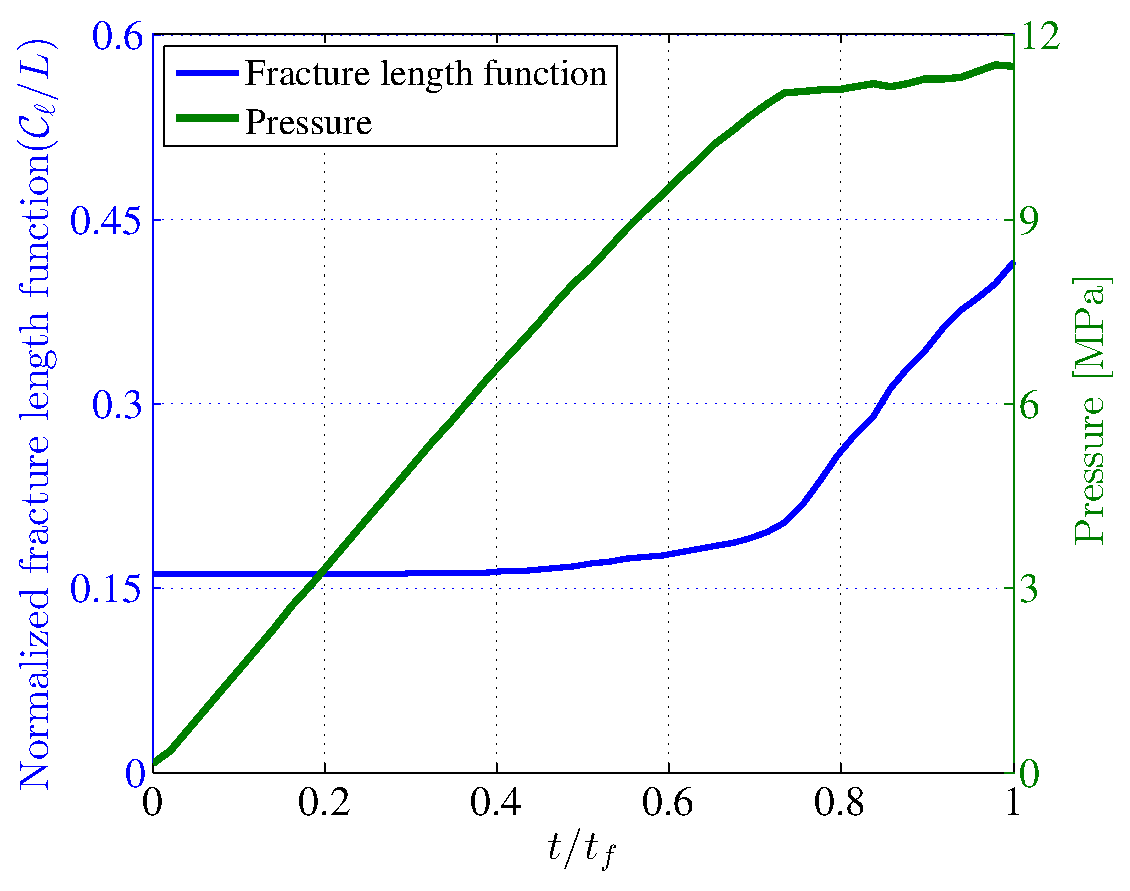
\includegraphics[width=0.6\textwidth]{Fracturelength_pressureboreholes_sigma_2}
    \caption{ The pressure at the top of the borehole (green line), and the fracture length function (blue line) as functions of time. The time when there is a sudden change of slope in $\mathcal{C}_{\ell}$ assumes the time corresponding to the breakdown pressure ($t=0.72t_f$) and the corresponding breakdown pressure is $p_b =10.9$ MPa. This is in agreement with H-F and H-W analytical solutions.}
	\label{Fig:Gas_pressure_Length_Sigma_i}
\end{figure}

Figure \ref{Fig:Gas_snapshots} shows the evolution of phase field diagram (left) and pressure profile (right) at different time steps. As seen, the fractures propagate along a straight line, and the pressure profile is accordingly distributed with the highest gradient around the borehole.

Next, we aim to calculate the breakdown pressure $p_b$, the pressure value when %at which the rapid drop in the injection pressure occurs and with 
the fractures start to propagate.
Figure \ref{Fig:Gas_pressure_Length_Sigma_i} illustrates the pressure evolution at the top of the borehole and the fracture length function. To estimate the breakdown pressure, first we output the fracture length with regard to \eqref{Eq:Gamma_ell}.  Then, we obtain the time when the slope suddenly changes in the fracture length function ($\mathcal{C}_{\ell}$), which is the time corresponding to the breakdown pressure (here $t\approx 0.72t_f$). Hence the breakdown pressure reads $p_b =10.9$ MPa. This value for $p_b$ is in agreement with H-F and H-W analytical solutions. Also, our results agree  with experiments results of Ishida \emph{et al.}~\cite{ishida2012acoustic} within 30\%, see Table \ref{Tab:preakdown_ISO_insitustress} and the next paragraph for more elaborations. 
%To validate our code we compare the numerical breakdown pressure with classical solutions$\cdots$
\begin{table}[htbp]
	\centering
	\caption{Breakdown pressure of numerical test and analytical solutions for $\sigma_1=\sigma_3=1$ MPa.}
	\begin{tabular}{l c c c c}
		\hline 
		& Numerical & H-F solution & H-W solution & Experimental \cite{ishida2012acoustic}  \\
		\hline 
		$p_b$ (MPa) & 10.9 & 11 &  9.1 & 8.44\\
		\hline      
	\end{tabular}
	\label{Tab:preakdown_ISO_insitustress}
\end{table}

\paragraph{Classical solutions of breakdown pressure} There exist two classical expressions to calculate the breakdown pressure. In the case without poroelastic effect the rock deformation does not penetrate into the pressurized fracture, the Hubbert-Willis (H-W) solution applies \cite{hubbert1972mechanics}:
\begin{equation*}
    p_b =3 \sigma_{3}- \sigma_{1}+\sigma_T,
\end{equation*}
in which the rock is assumed to be an elastic medium. When the porous medium is set, the Haimson-Fairhurst (H-F) solution is preferred \cite{haimson1967initiation}:
\begin{equation*}
    p_b=\dfrac{3\sigma_{3}- \sigma_{1}+\sigma_T+p_0}{1+\dfrac{\nu}{1-\nu}\alpha},
\end{equation*}
where we denote by $p_b$ the breakdown fluid pressure, $\sigma_{3}$, and $\sigma_{1}$ are the minimum and maximum principal stresses, respectively, and $\sigma_T$ is the rock's tensile strength.

\paragraph{Effect of $N$, $h$, and $\ell$ on the breakdown pressure}
Here we aim to study how the number of time steps $N$, the mesh size $h$, and the regularization length scale $\ell$ affect the value of breakdown pressure. As seen in Figure \ref{Fig:Gas_Pressure_parameters}, the plots show similar numerical results for the pressure evolution.

%\begin{figure}
%    \centering
%    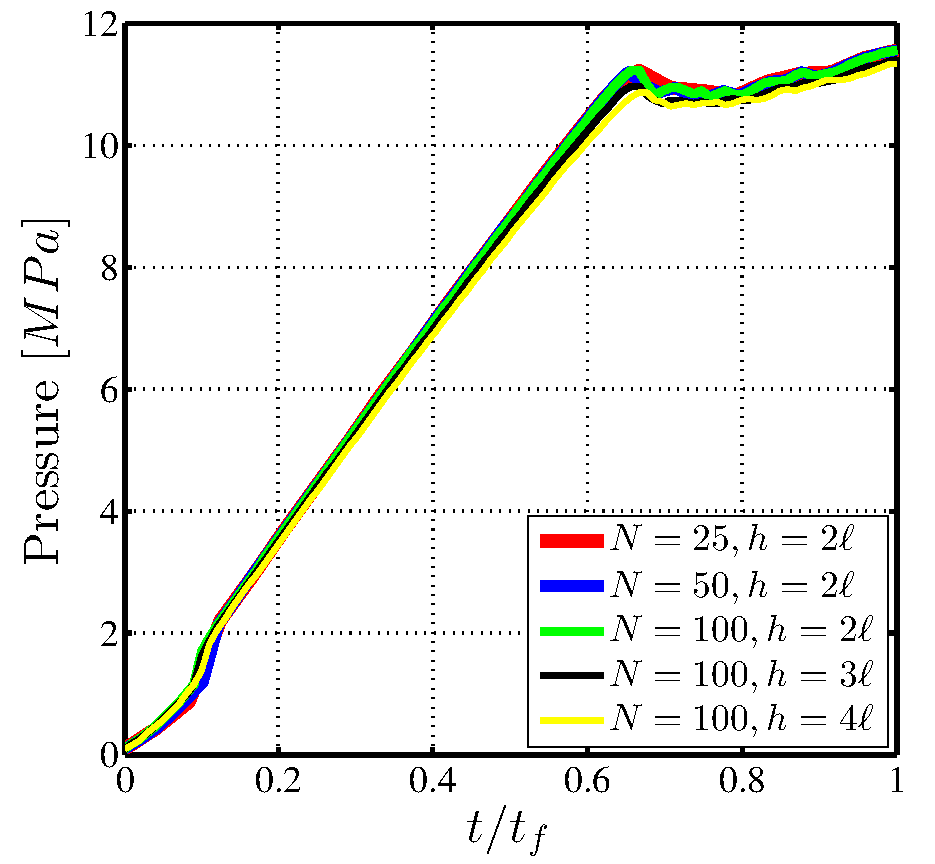
\includegraphics[width=0.6\textwidth]{breakdownpressure_diff_ell_loadstep}
%        \caption{The pressure profile at the top of borehole for different {time steps, $N$}, and $\ell$.}
%    \label{Fig:Gas_Pressure_parameters}
%\end{figure}


\begin{figure}
    \centering
    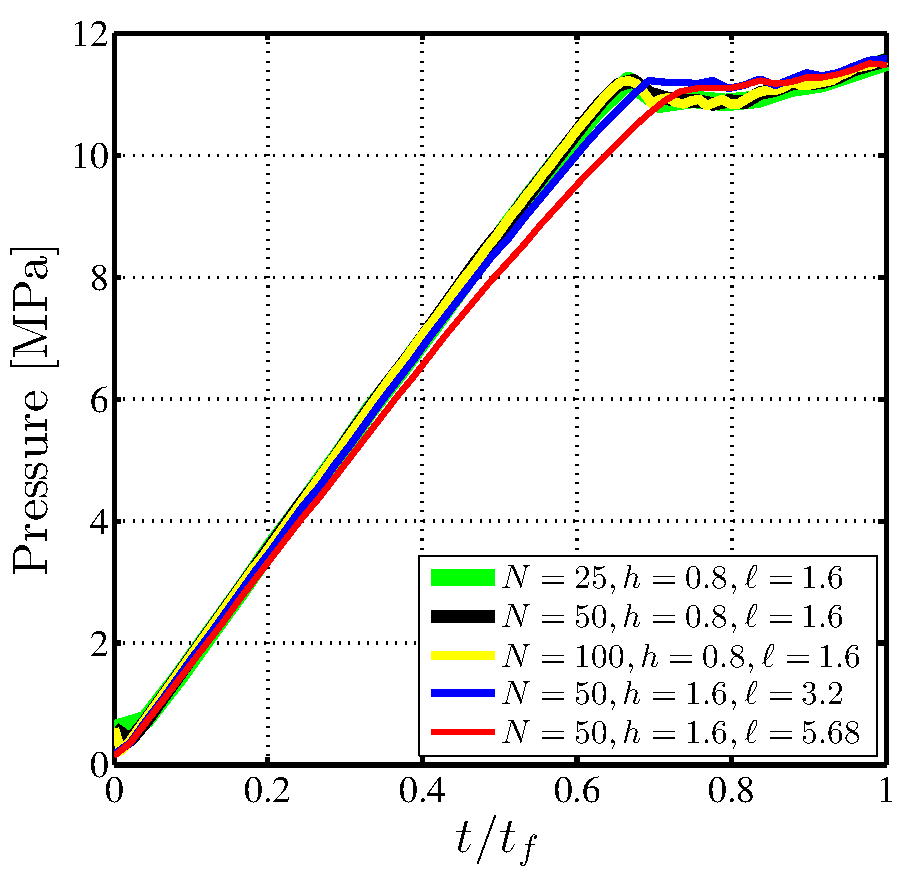
\includegraphics[width=0.6\textwidth]{breakdownpressure_diff_ell_loadstep_2}
        \caption{Evolution of the pressure at the top of the borehole for different numbers of time steps $N$, mesh size $h$, and $\ell$.}
    \label{Fig:Gas_Pressure_parameters}
\end{figure}

%\todo[inline]{YS: Effect of the deviatoric part of the \emph{in situ} stress?\\Vahid: Changed.}
\paragraph{Breakdown pressure result of an anisotropic \emph{in situ} stress} In this example we set the maximum ($\sigma_1=3$ MPa) and minimum ($\sigma_3=2$ MPa)  \emph{in situ} stress. The other input data and boundary conditions are the same as aforementioned.

The pressure at the top of the borehole and the fracture length function, \eqref{Eq:Gamma_ell}, at different stages are  illustrated in Figure \ref{Fig:Gas_pressure_Length_Sigma_diff}. The breakdown time ($t\approx 0.77t_f$) and the corresponding breakdown pressure is $p_b =11.9$ MPa, see Table \ref{Tab:preakdown_anISO_insitustress}.

\begin{table}[htbp]
    \centering
    \caption{Breakdown pressure of numerical test and analytical solutions for $\sigma_1=3$ MPa and $\sigma_3=2$ MPa.}
    \begin{tabular}{l c c c}
    \hline 
           & Numerical & H-F solution & H-W solution \\
    \hline 
           $p_b$ (MPa)& 11.9 & 14 &  9.8 \\
    \hline      
    \end{tabular}
    \label{Tab:preakdown_anISO_insitustress}
\end{table}

\begin{figure}[htbp]
    \centering
    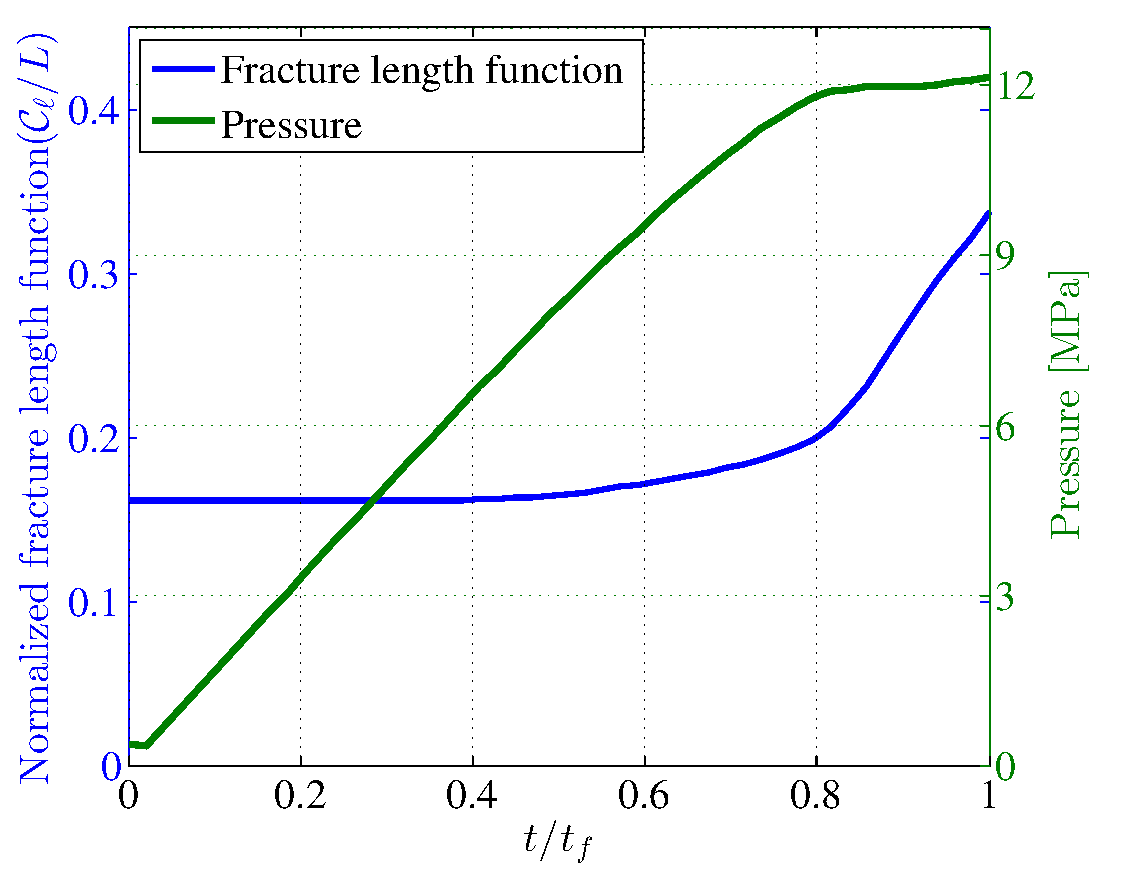
\includegraphics[width=0.6\textwidth]{Fracturelength_pressureboreholes_sigma_diff_2}
        \caption{The pressure at the top of the borehole (green line) and  the fracture length function (blue line) versus time for deviatoric \emph{in situ} stress are shown. The time ($t\approx 0.8t_f$) when there is a change of slope in the fracture length function ($\mathcal{C}_{\ell}$) should correspond to the breakdown pressure ($p_b=11.9$ MPa).}
    \label{Fig:Gas_pressure_Length_Sigma_diff}
\end{figure}

%\todo[inline]{Mostafa: Do we need keep this example? Since the results do not agree with experiments. Actually, the experiments indicate that the breakdown pressure is different for different fluids ($\mu$).\\Vahid: I added a few sentences to explain the case.}
\paragraph{Effect of dynamic viscosity on breakdown pressure} We conduct several numerical examples to investigate the effect of dynamic viscosity $\mu$ on the breakdown pressure $p_b$. 
In this set of examples an effective mesh size, the mesh size near the borehole or the fractures, $h\approx 1.6$ mm is adopted. Also, we set $\ell=2h$. In Figure \ref{Fig:Gas_Pressure_viscosity} we plot the pressure evolution up to the time when  $\mathcal{C}_\ell(t)$ changes slope, so that the end points correspond to the breakdown pressures. The results indicate that $p_b$ is approximately the same for different fluid viscosities, but the time when breakdown pressure reaches  is different. Figure \ref{Fig:Gas_Pressure_viscosity} demonstrates that the rock will break earlier for the fluid with bigger dynamic viscosity. Also it shows that regardless of the fracturing fluid, the breakdown pressure is slightly the same for all cases. This is in accordance with the physics that the breakdown pressure normally reflects the strength of the solid. However, Wang \emph{et al.}~\cite{wang2018influence} reported different breakdown pressures for different fluids which also agrees with some experiments \cite{ishida2012acoustic, ishida2016features}. We believe this discrepancy demands further research.

%\begin{figure}
%    \centering
%    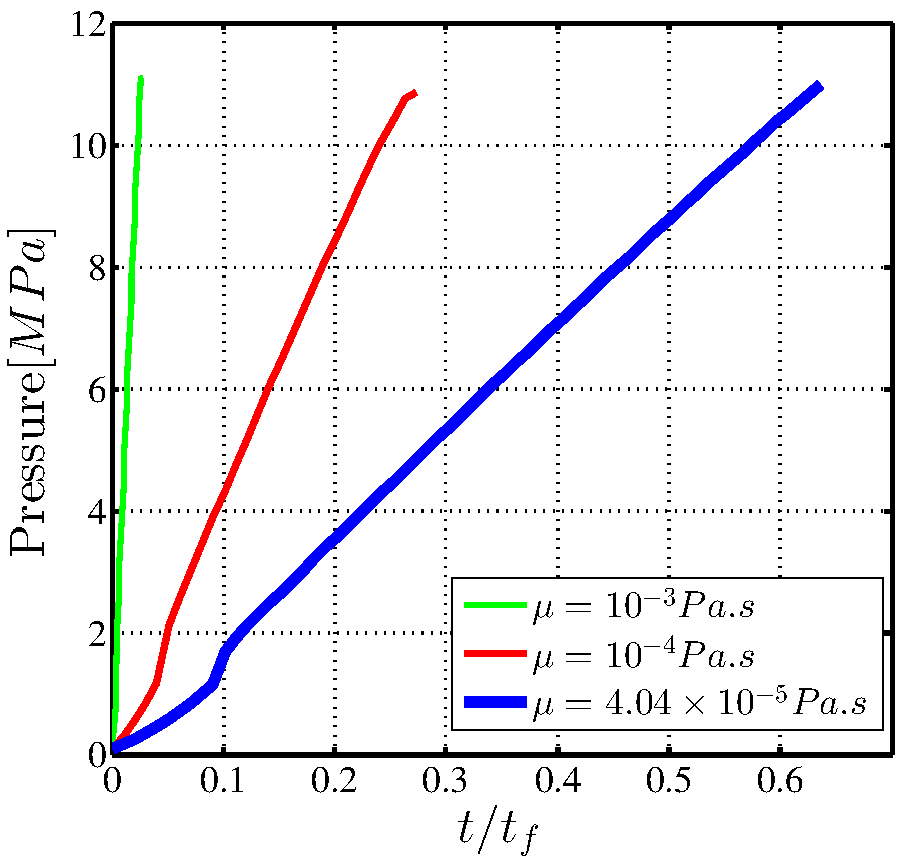
\includegraphics[width=0.6\textwidth]{breakdown_diff_viscosity}
%         \caption{The pressure profile at the top of borehole for different $\mu$. As seen, even though $p_b$ is the same for different fracturing fluids, by increasing $\mu$, the breakdown pressure is reached in earlier time.}
%    \label{Fig:Gas_Pressure_viscosity}
%\end{figure}

%\todo[inline]{YS: Problems with Figure \ref{Fig:Gas_Pressure_viscosity}: $t_c$ should be $t_f$, and also the second legend shall be $\mu=1.00\times10^{-4}$ Pa$\cdot$s.\\
%Mostafa: It's edited}

\begin{figure}[htbp]
    \centering
    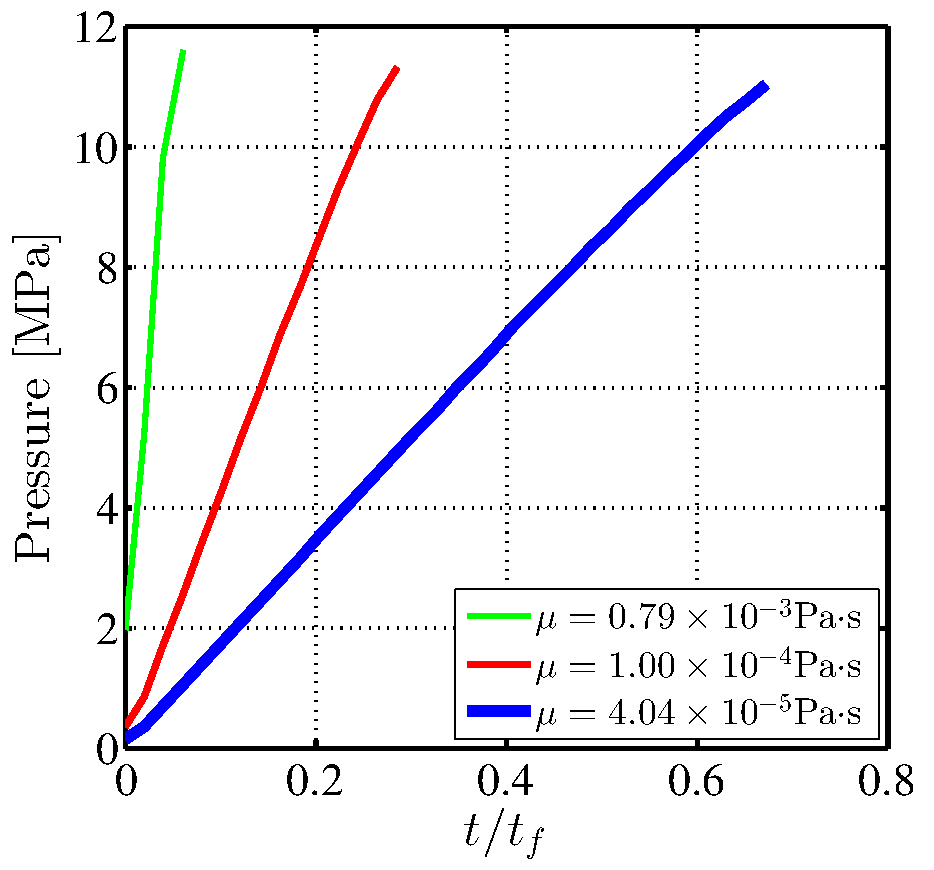
\includegraphics[width=0.6\textwidth]{breakdown_diff_viscosity_2}
         \caption{Evolution of the pressure at the top of the borehole for different $\mu$'s. As seen, even though $p_b$ is the same for different fracturing fluids, by increasing $\mu$, the breakdown pressure is reached earlier.}
    \label{Fig:Gas_Pressure_viscosity}
\end{figure}
\section{Conclusions}\label{sec:concl}
We have proposed \added{and verified} a phase field approach to simulate CO$_2$ fracturing, with CO$_2$ treated as a compressible fluid. \replaced{In one of the numerical examples, the}{The} breakdown pressure agrees well with widely used analytical solutions. Also, the results agree with experimental results within 30\%. While this work represents the first of its kind, potentially the phase field approach allows complicated modeling of fracture initiation and branching.
%\input{section_6_Conclusions}
\clearpage
\appendix
%\renewcommand{\theequation}{A-\arabic{equation}}
%    % redefine the command that creates the equation no.
%\setcounter{equation}{0}  % reset counter  
%\section{Verification of the method}\label{Sec:App}
This appendix devotes to a verification of our implementation of the present phase field method for CO$_2$ fracturing. To this end, we present three examples with exact or otherwise trusted solutions to study how our outputs are in accordance with the analytical solutions and other works.

\subsection{Single-edge-notched tension test}
We first investigate a square plate with a horizontal {initial} crack at the middle height starting from the left end and ending at the plate center. The geometric setup is depicted in Figure \ref{Fig:Notched_geometry}. To capture the crack pattern properly, the mesh is refined in areas where the crack is expected to propagate, i.e., in the center strip of the specimen. In effect, for a discretization with 105,352 standard $P_1$ elements, an effective element size of $h\approx 5\times 10^{-3}$ mm is obtained in the critical zone. The specimen is under a direct tension test, in which a monotonically increasing displacement with constant increments $\Delta\bm{u}=6 \times 10^{-5}$ mm is imposed on the top edge while the bottom edge is fixed. In this example, the evolution is simulated for 100 uniform time steps so that a final deformation of $6\times 10^{-3}$ mm is reached. We will adopt the values of the material parameters given in Table \ref{Tab:Notched_input}. Note that all our models are implemented with the AT1 model.
%Also, the {regularization parameter} is set to be $l=\dots~mm$.
\begin{figure}[htbp]
    \centering
    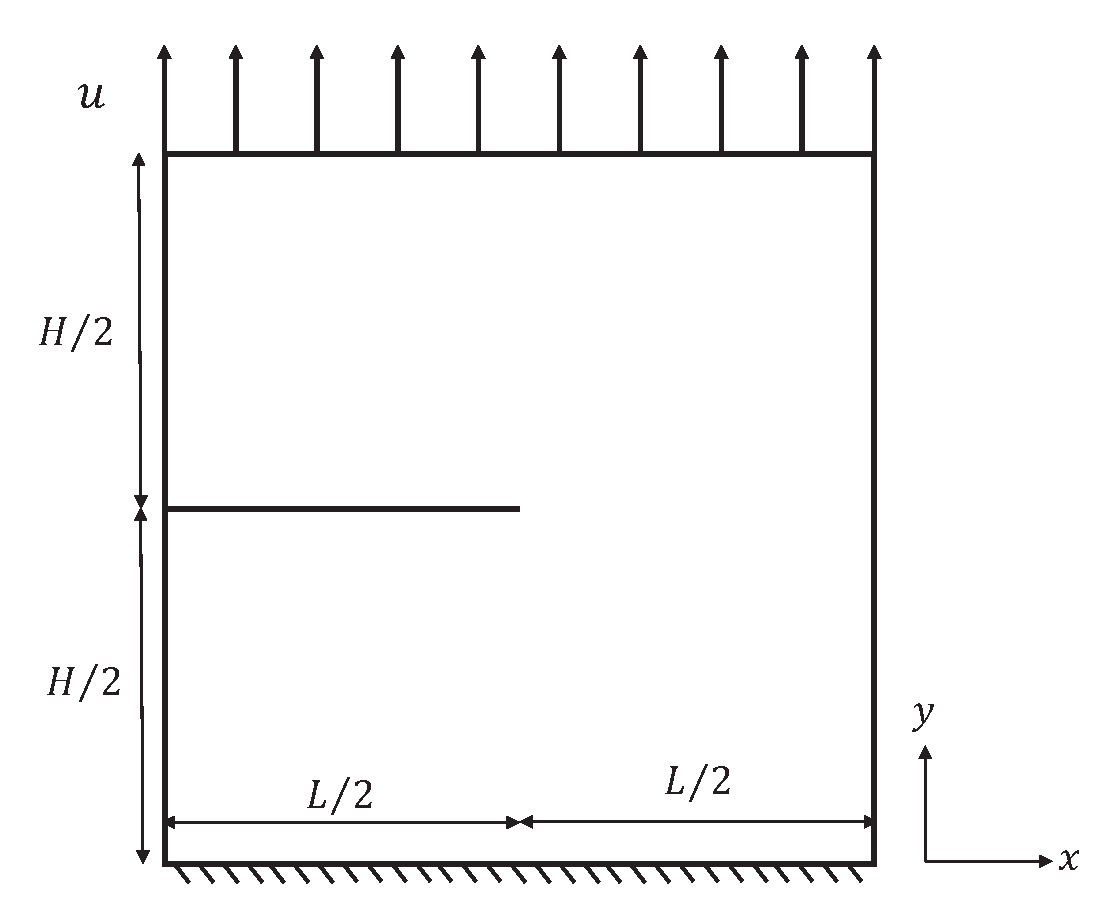
\includegraphics[width=80mm]{edgeNotch}
    \caption{Schematic of a cracked square plate (unit: mm) under a single-edge-notched tension test. 
    A monotonically increasing displacement with constant increments $\Delta\bm{u}=6\times 10^{-5}$ mm is applied on the top edge while the bottom edge is fixed.}
    \label{Fig:Notched_geometry}
\end{figure}

\begin{table}[htbp]
    \centering
    \caption{Cracked square plate under a tension test: Material parameters \cite{ambati2015review}}
    \begin{tabular}{l c c c}
    \hline 
         Parameters & symbol & unit& value \\
    \hline 
         Young's modulus & $E$ &MPa&  210$\times 10^{3}$\\
         Poisson's ratio & $\nu$ &$-$&  0.3\\
         Critical energy release rate & $g_c$ &MPa$\cdot$mm&  2.7\\
            \hline      
    \end{tabular}
    \label{Tab:Notched_input}
\end{table}

The resulting crack patterns at different stages of the deformation for two fixed regularization length scales $\ell = \ell_1 = 1\times 10^{-2}$ mm and $\ell = \ell_2=2 \times 10^{-2}$ mm are illustrated in Figure \ref{Fig:Notched_snapshots}. 
As expected, in both simulations, the fracture propagates straightforward to the end. This straight crack topology agrees well with the results in \cite{miehe2010thermodynamically}. Also as seen, the resulting crack pattern with the smaller $\ell$ looks sharper.

\begin{figure}[!htb]
    \centering
    \subfloat[]{
    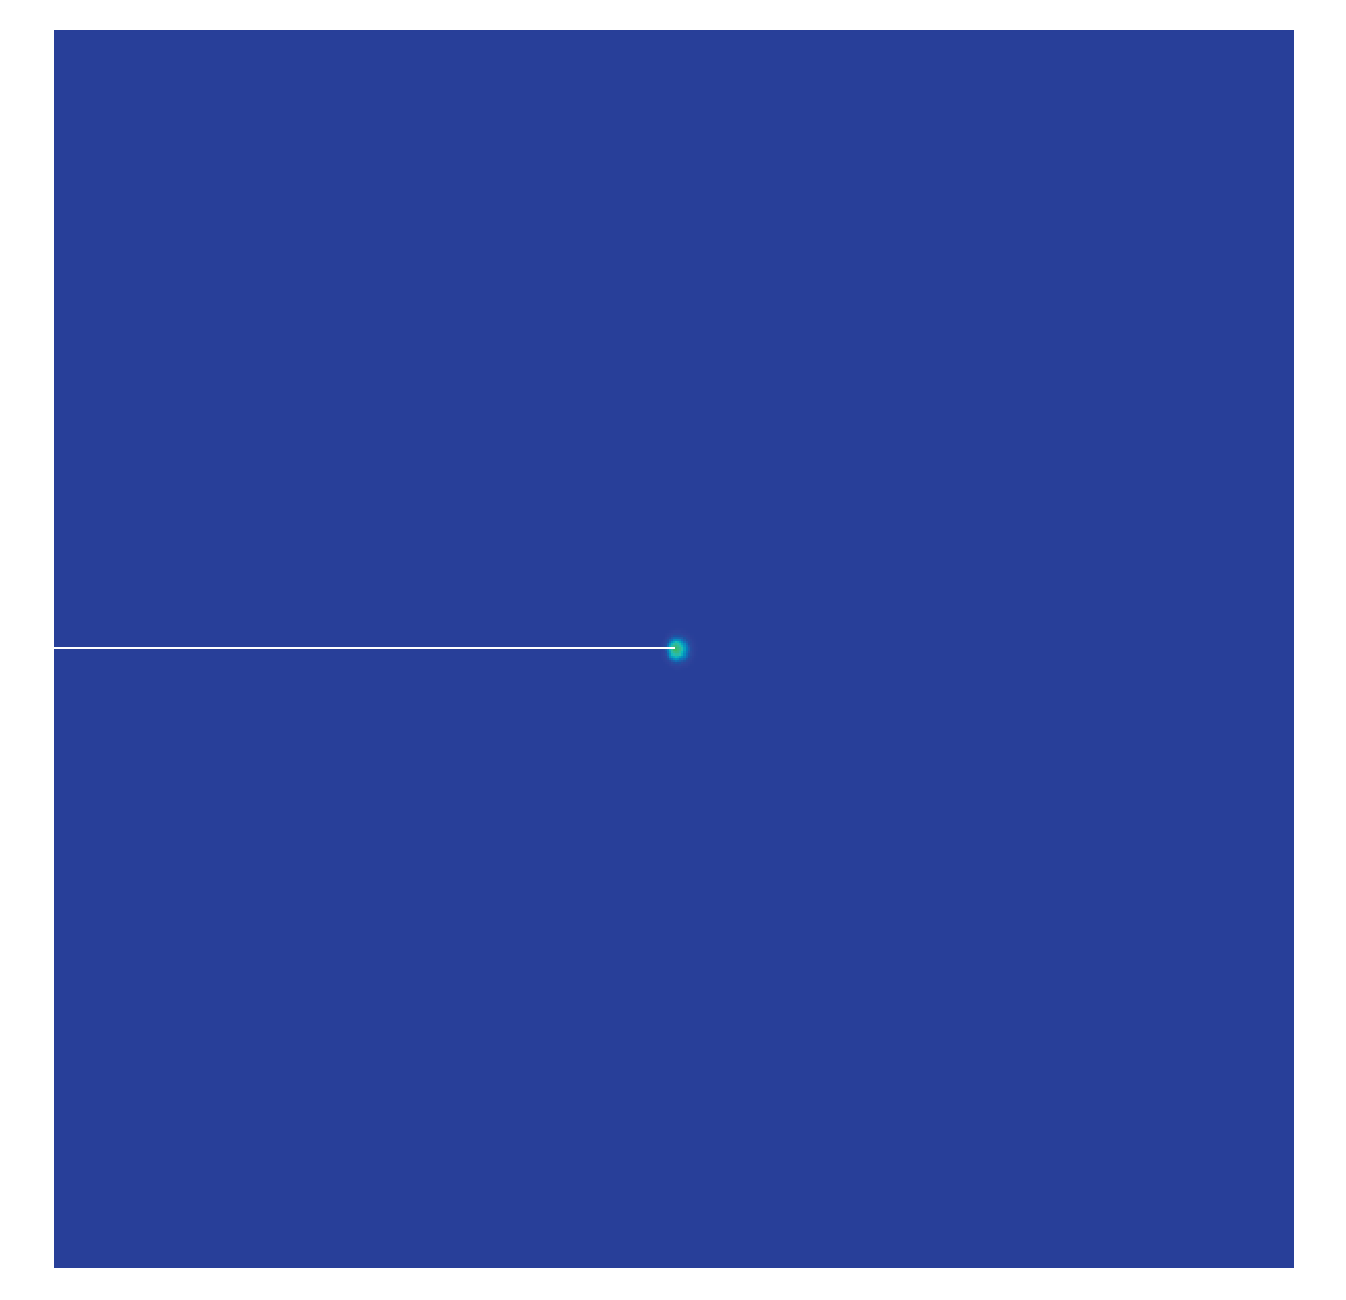
\includegraphics[width=0.4\textwidth]{snapshot_l2h_t92.eps}
    \label{Fig:Notched_lenght_scale_2h_i}}
    \subfloat[]{
    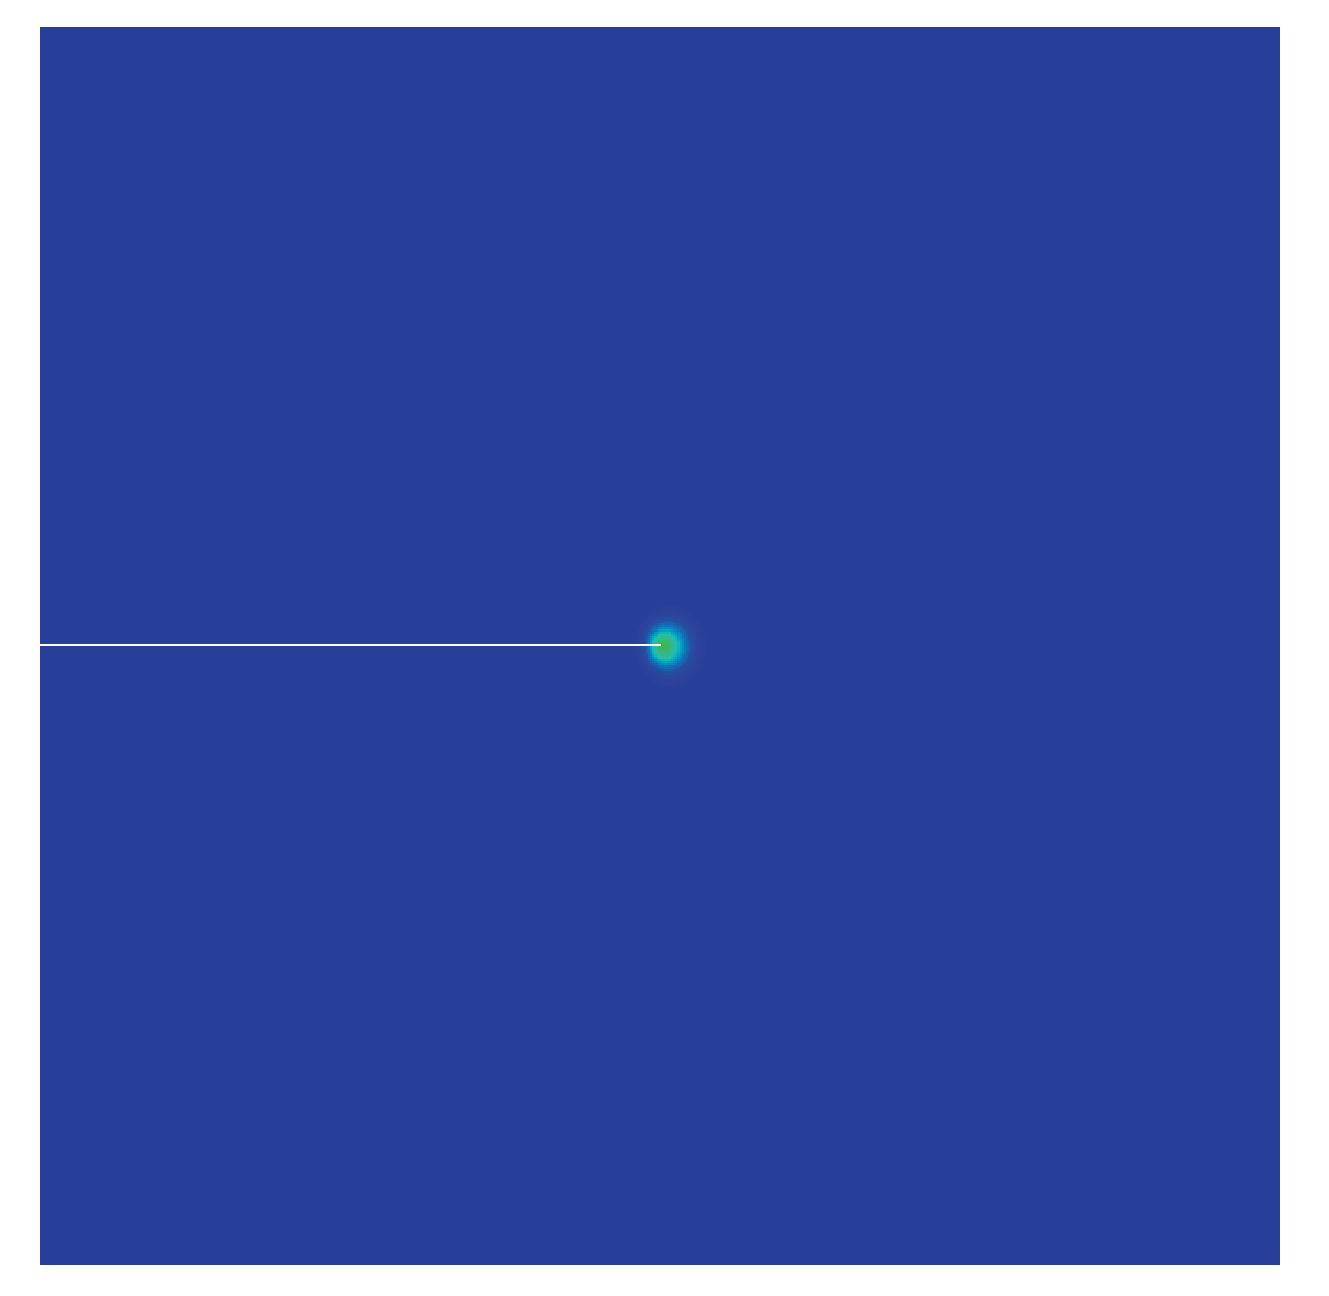
\includegraphics[width=0.4\textwidth]{snapshot_l4h_t92.eps}
    \label{Fig:Notched_lenght_scale_4h_i}}\\
    \subfloat[]{
    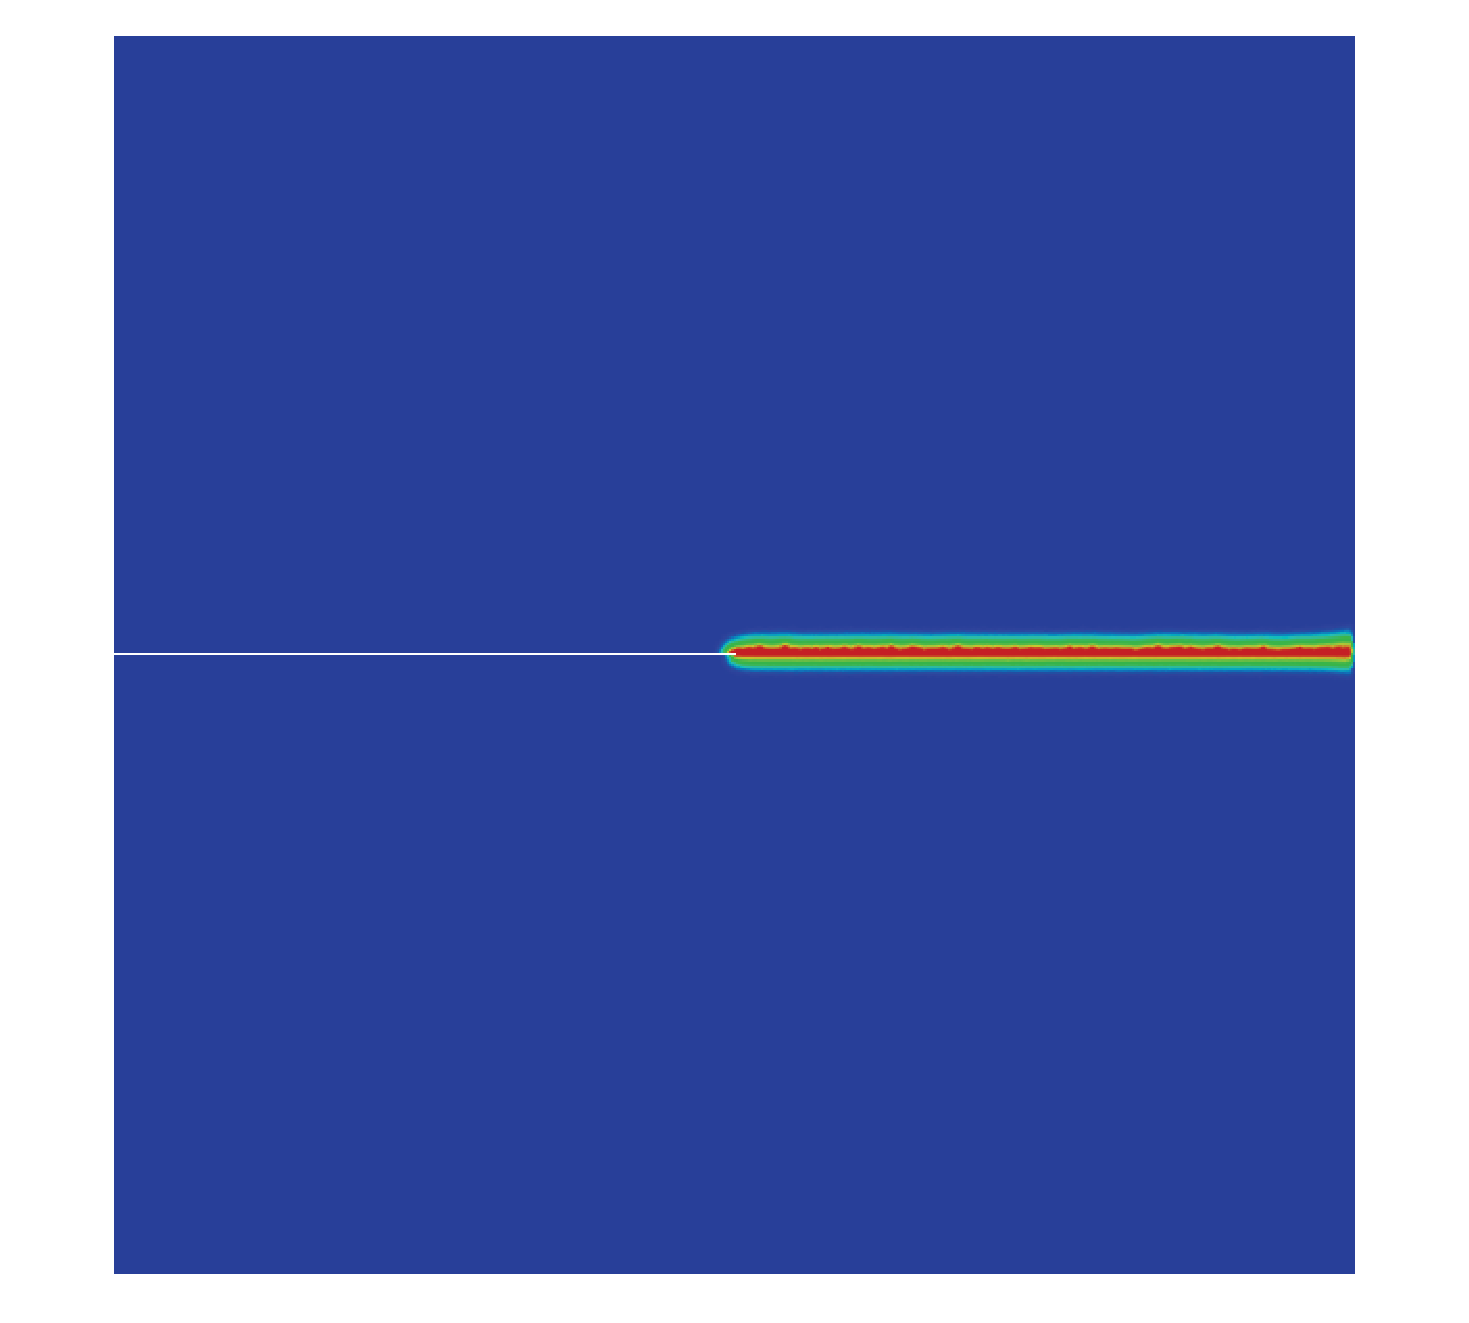
\includegraphics[width=0.4\textwidth]{snapshot_l2h_t93.eps}
    \label{Fig:Notched_lenght_scale_2h_ii}}
    \subfloat[]{
    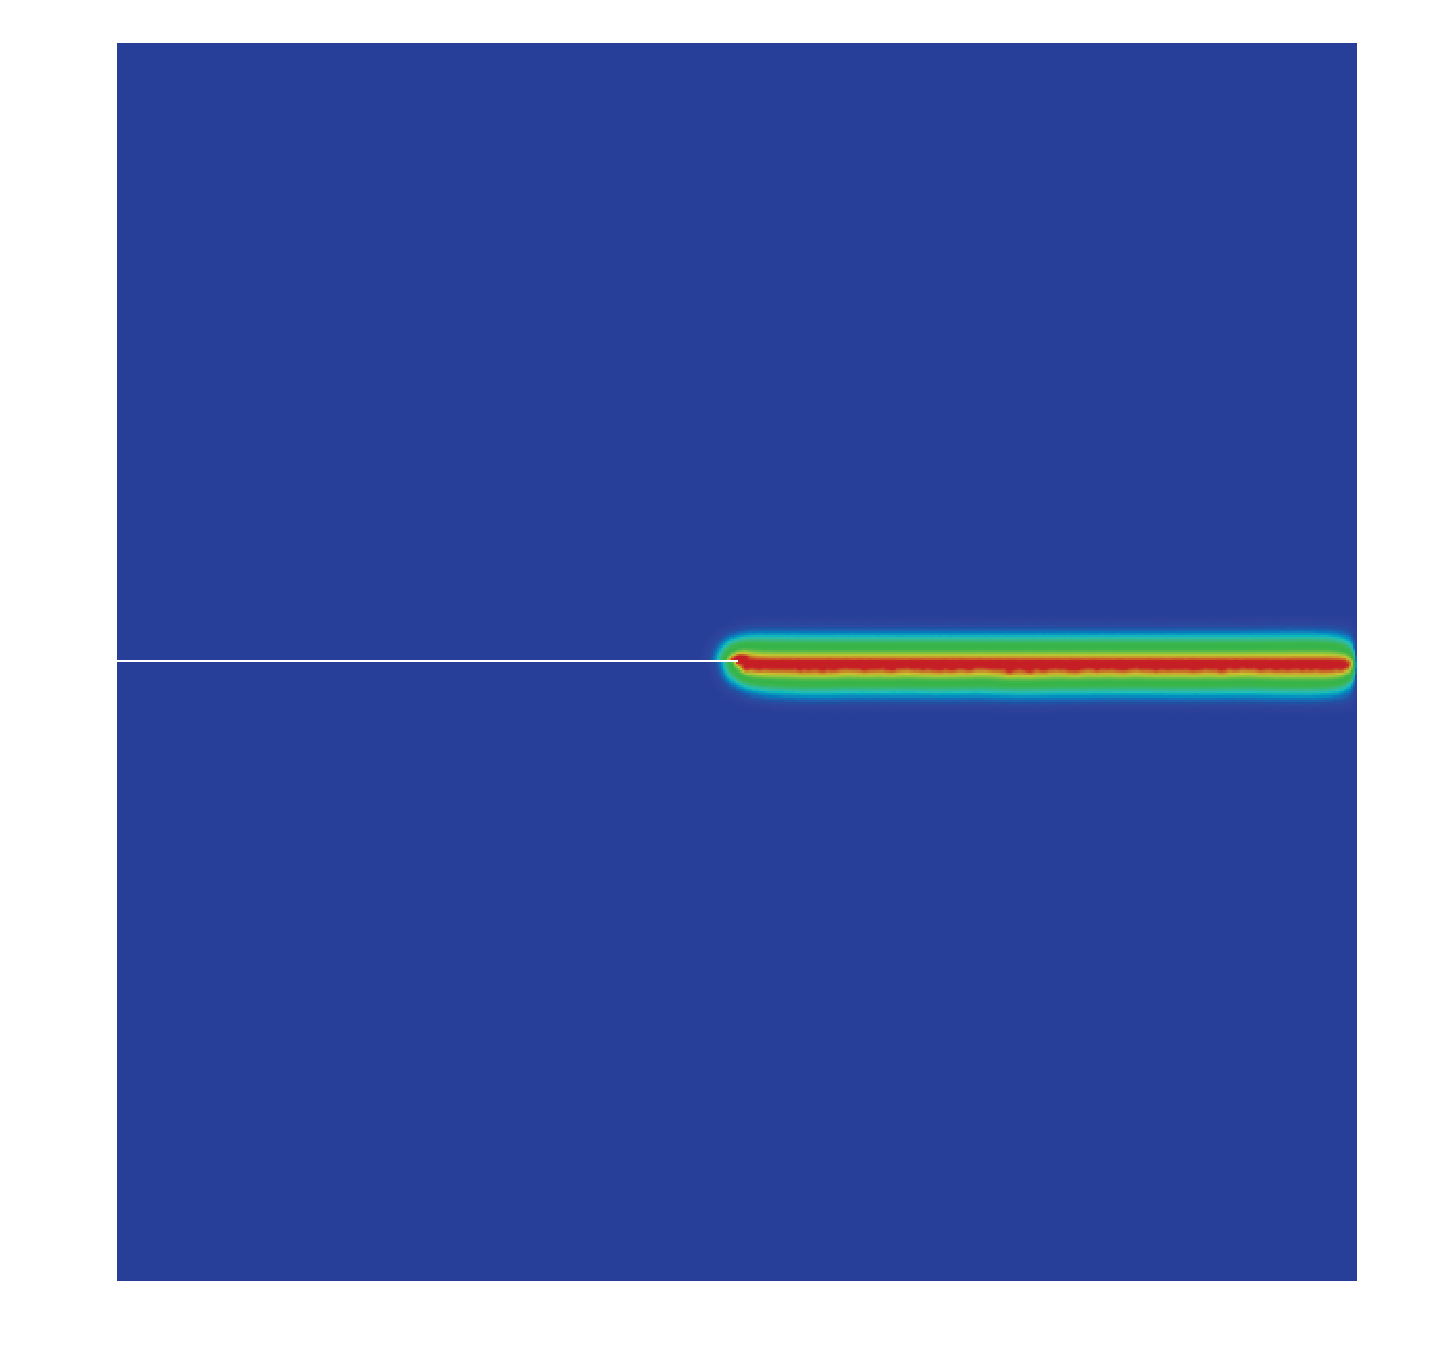
\includegraphics[width=0.4\textwidth]{snapshot_l4h_t93.eps}
    \label{Fig:Notched_lenght_scale_4h_ii}}\\
    \subfloat[]{
    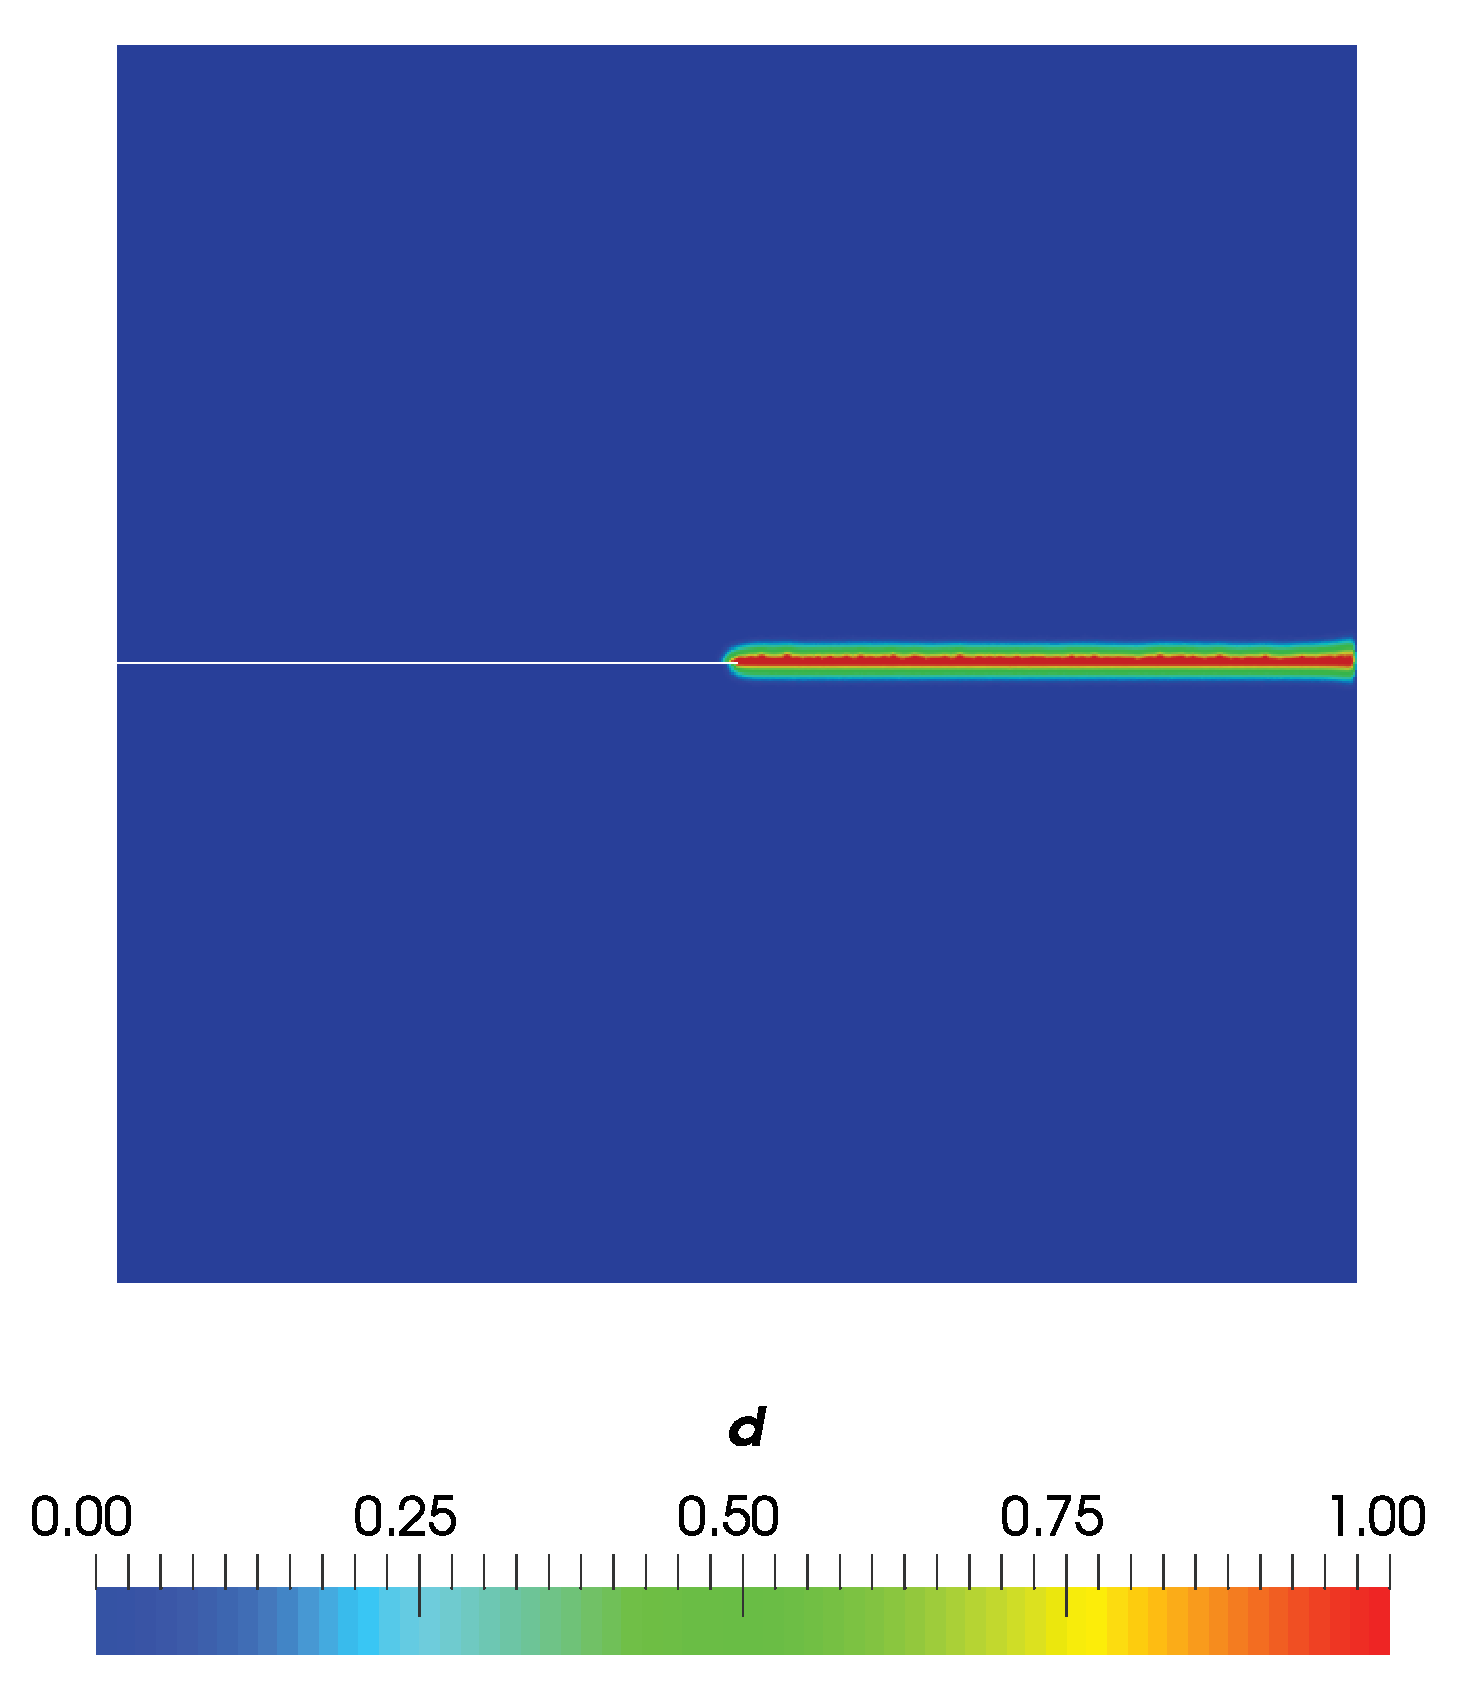
\includegraphics[width=0.4\textwidth]{snapshot_l2h_t99.eps}
    \label{Fig:Notched_lenght_scale_2h_iii}}
    \subfloat[]{
    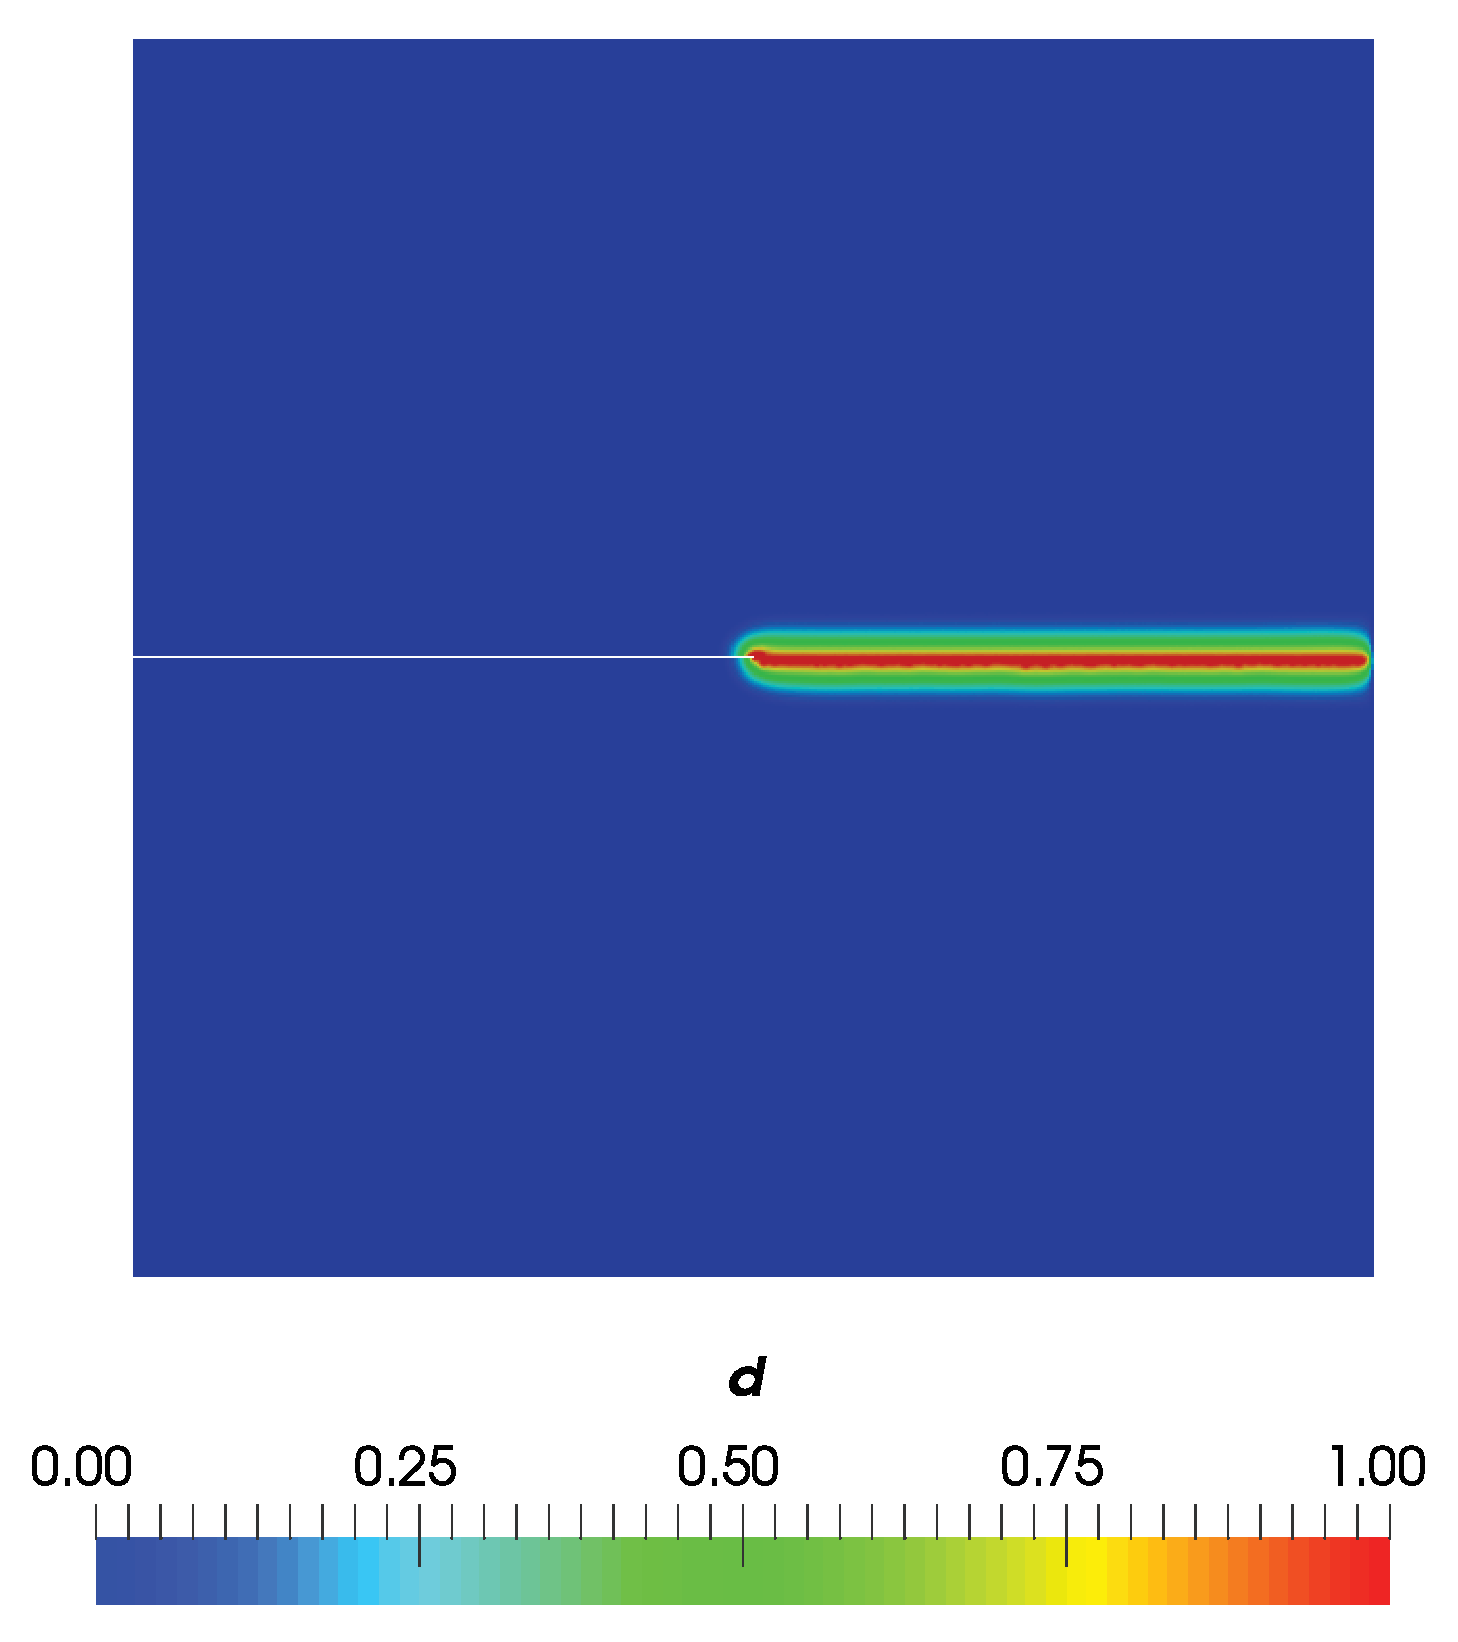
\includegraphics[width=0.4\textwidth]{snapshot_l4h_t99.eps}
    \label{Fig:Notched_lenght_scale_4h_iii}}

    \caption{Cracked square plate under a tension test {with two different regularization length scales $\ell=\ell_1 = 10^{-2}$ mm $\approx 2h$ (left) and $\ell=\ell_2 = 2\times 10^{-2}$ mm $\approx 4h$ (right)}. Both simulations are done with 100 uniform time steps with $\Delta\bm{u}= 6 \times 10^{-5}$ mm (See also Table \ref{Tab:Notched_input} for the input values). Phase field contours at three different stages $\bm{u}=5.52 \times 10^{-3}$ mm (\ref{Fig:Notched_lenght_scale_2h_i},\ref{Fig:Notched_lenght_scale_4h_i}), $\bm{u}=5.58 \times 10^{-3}$ mm (\ref{Fig:Notched_lenght_scale_2h_ii},\ref{Fig:Notched_lenght_scale_4h_ii}), and $\bm{u}=6 \times 10^{-3}$ mm (\ref{Fig:Notched_lenght_scale_2h_iii},\ref{Fig:Notched_lenght_scale_4h_iii}) are shown in deformed configurations with the deformations scaled. The initial cracks are explicitly imposed, so in the deformed configuration it appears as a white line. As expected, we observe a straight crack pattern in both cases.
    }
    \label{Fig:Notched_snapshots}
\end{figure}

We also output the load-deflection curves for the two setups of Figure \ref{Fig:Notched_lenght_scale}. As seen, both models will result in similar trends. Hence, the effect of $\ell$ on the response is small in this range.

\begin{figure}[htbp]
    \centering
    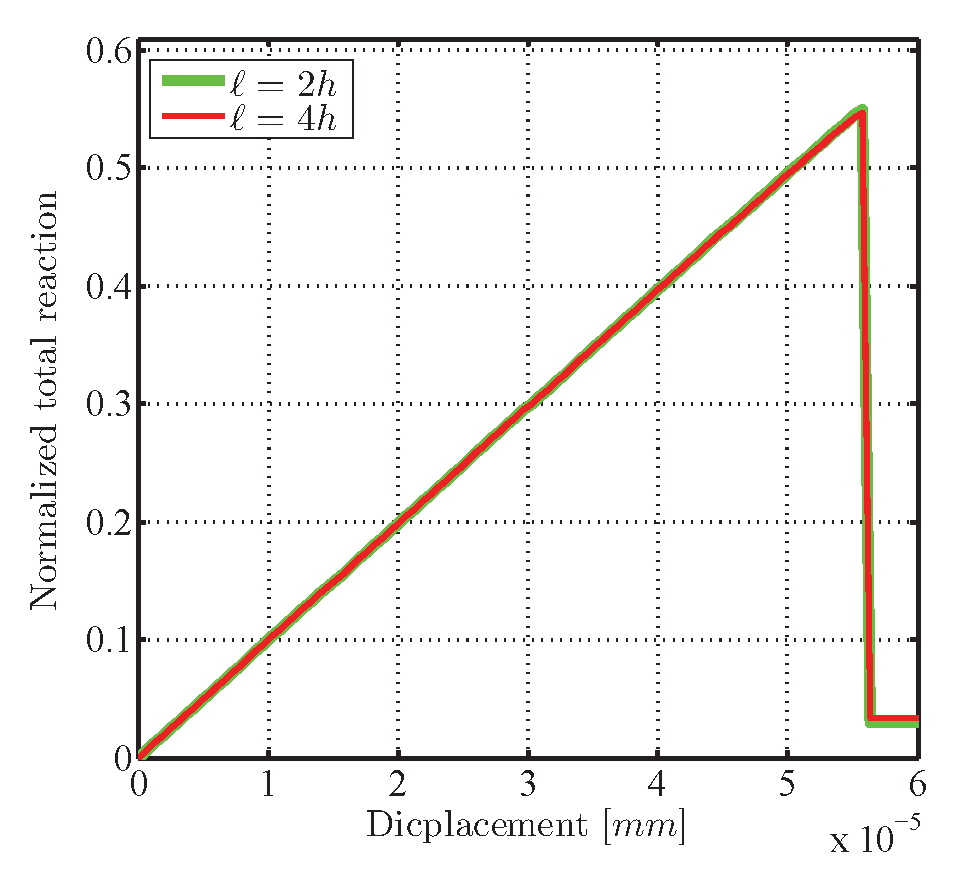
\includegraphics[width=0.6\textwidth]{Force_ELL_fracture}
    \caption{Cracked square plate under a tension test {with two different regularization length scales $\ell=\ell_1 =  10^{-2}$ mm $\approx 2h$ (red) and $\ell=\ell_2= 2\times 10^{-2}$ mm $\approx 4h$ (green)}. Load-deflection curves for both $\ell_1$ and $\ell_2$ are obtained. Both simulations are done with 100 load steps with $\Delta\bm{u}=6 \times 10^{-5}$ mm. The total reaction is normalized by the one in the case without any crack or phase field evolution. Both models give rise to similar trends so the effect of changes in $\ell$ is small within this range. Note that the reaction highly decreases at the 93rd time step where the crack starts to propagate.}
    \label{Fig:Notched_lenght_scale}
\end{figure}

%In order to point out the effects that arise due to the choice of the methods $AT1$ or $AT2$, Figure \ref{Fig:Notched_law_model} depicts the obtained load-deflection curves. Note that here we take $\ell= \added{4h}$. \added{As seen, both methods result in similar trends, although the $AT1$ method is having the higher pick value.}

%\begin{figure}[htbp]
%    \centering
 %   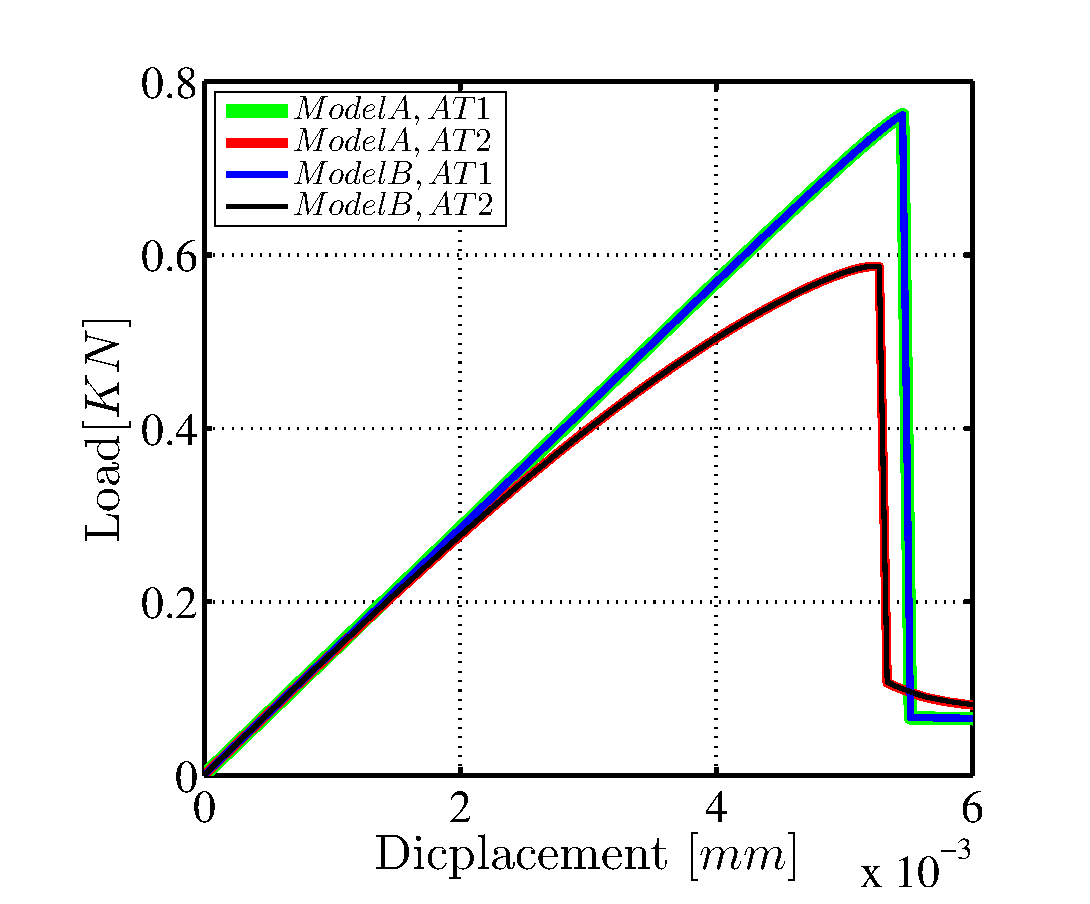
\includegraphics[width=100mm]{Force_LAW_MODEL_fracture.eps}
%    \caption{Cracked square plate under a tension test {with $\ell=\added{4h}~\text{mm}$.} Load-deflection curves for two different methods $AT1$ and $AT2$ are obtained. Both simulations are done with a number of \added{100} time steps with $\Delta\bm{u}= \added{0.006}~\text{mm}$. The total reaction is normalized by the one in the case without any crack or phase field evolution. The methods AT1 and AT2 show slightly different values while following similar trend. \added{Note that the total reaction highly decreases at the \dots-th time step where the crack starts to propagate.}}
%    \label{Fig:Notched_law_model}
%\end{figure}

\subsection{Poroelastic response of a borehole}
This example  aims to study the effect of fluid pressurization on the poroelastic response around the borehole.
It was first studied by {Detourney and Cheng} \cite{detournay1988poroelastic} (see also \cite{wang2018influence, lu2013microcrack}). Consider a plane strain hydraulic fracturing problem where there is a square plate containing a central borehole. The geometry and the loading conditions in this example are the same as Figure \ref{Fig:Gas_geometry}. The far-field \emph{in situ} stress is set to zero in this example. Note also that $d\equiv0$, i.e., there is no preexisting crack in the specimen and we do not allow for any nucleation of the fracture as the rock strength is assigned a very large value. A discretization with 28,140 standard $P_1$ elements is applied to the problem. To capture the high gradient of pressure near the borehole, the mesh is refined in that area so that an effective mesh size of $h\approx 0.15$ mm is adopted. The fluid is slightly compressible, and we set the fluid pressure in the borehole to $1$ MPa. The other material properties are prescribed according to Table \ref{Tab:Borehole_input}.

Here, the governing equation for the slightly compressible flow is written as follows \cite{detournay1988poroelastic}:
\begin{equation*}%\label{Eq:ap2}
   \begin{aligned}
        \partial_t p+ M \nabla \cdot \left(\frac{k_0}{\mu} \nabla p\right)=0
    \end{aligned}
\end{equation*}
where $M=E\left( 1-\nu\right) /[\left(1+\nu \right)\left(1-2\nu \right)]$ is called the constrained modulus.
%\todo[inline]{Vahid: Mostafa, please add the formula for $M$ in place of dots.\\Mostafa: it's added\\YS: It may be just $\lambda$ or the bulk modulus.\\Mostafa: It seems that $M $ is different from first Lame constant or bulk modulus.}
\begin{table}[htbp]
    \centering
    \caption{Poroelastic response of a borehole: Material parameters}
    \begin{tabular}{l c c c}
    \hline 
         Parameters & symbol & unit& value \\
    \hline 
         Young's modulus & $E$ &MPa&  6000\\
         Poisson's ratio & $\nu$ &$-$&  0.34\\
         Biot coefficient & $\alpha$ &$-$&  1.\\
         Permeability & $k_0$ &mm$^2$&  1$\times 10^{-12}$\\
            \hline      
    \end{tabular}
    \label{Tab:Borehole_input}
\end{table}

Figure \ref{Fig:Borehole_porepressure} shows the distribution
of pore pressure around the borehole for three values of dynamic viscosity $\mu$ at early time $t=0.1$ s. Note that the horizontal axis is $(r-r_0)/r_0$, ranging from $0$ to $0.25$ in the direction of $\theta= \pi/2$. The simulation results are then compared to the analytical solution by Detourney and Cheng \cite{detournay1988poroelastic}.

Figure \ref{Fig:Borehole_tangential_stress} depicts the effect of dynamic viscosity on the effective tangential stress in the vicinity of the borehole at early time $t=0.1$ s.%\todo{YS: Any conclusion?}

\begin{figure}[htbp]
    \centering
    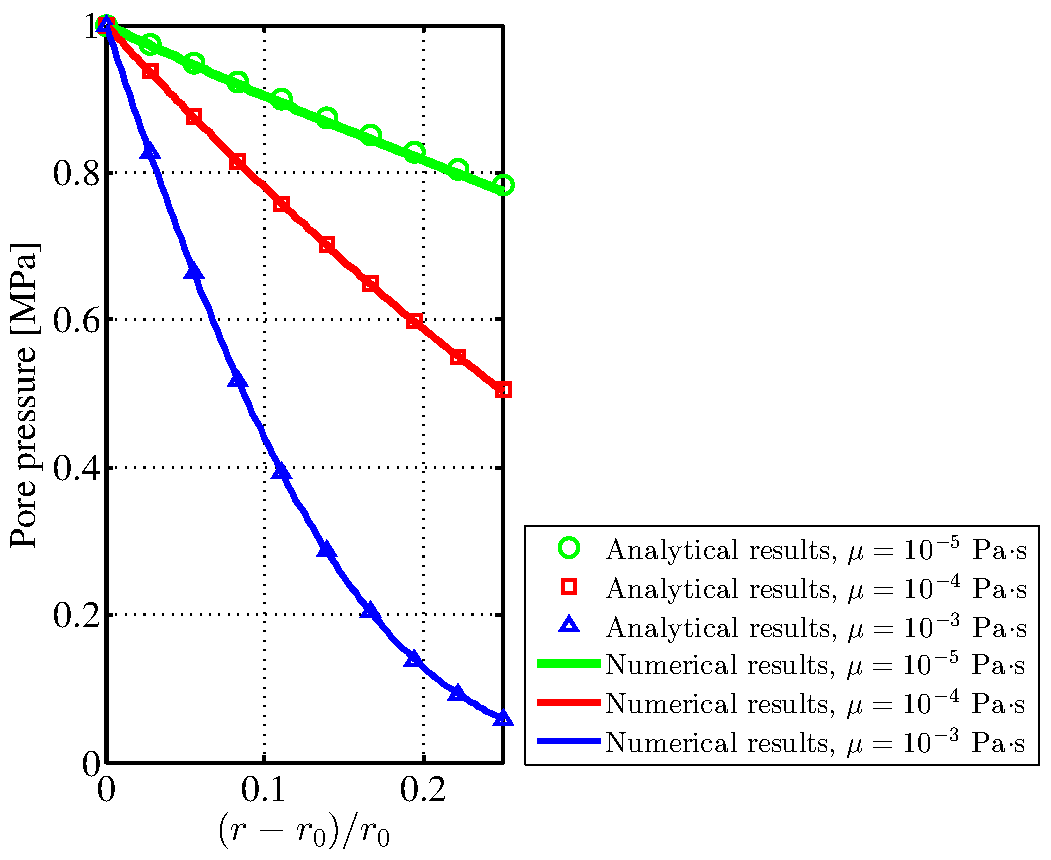
\includegraphics[width=0.8\textwidth]{verify_porepressure}
    \caption{Poroelastic response of a borehole. The distribution of pore pressure caused by fluid pressurization is shown around the borehole for three different dynamic viscosities $\mu$ at early time $t= 0.1$ s. As seen, the results are in good accordance with the analytical in \cite{detournay1988poroelastic}.}
    \label{Fig:Borehole_porepressure}
\end{figure}

\begin{figure}[htbp]
    \centering
    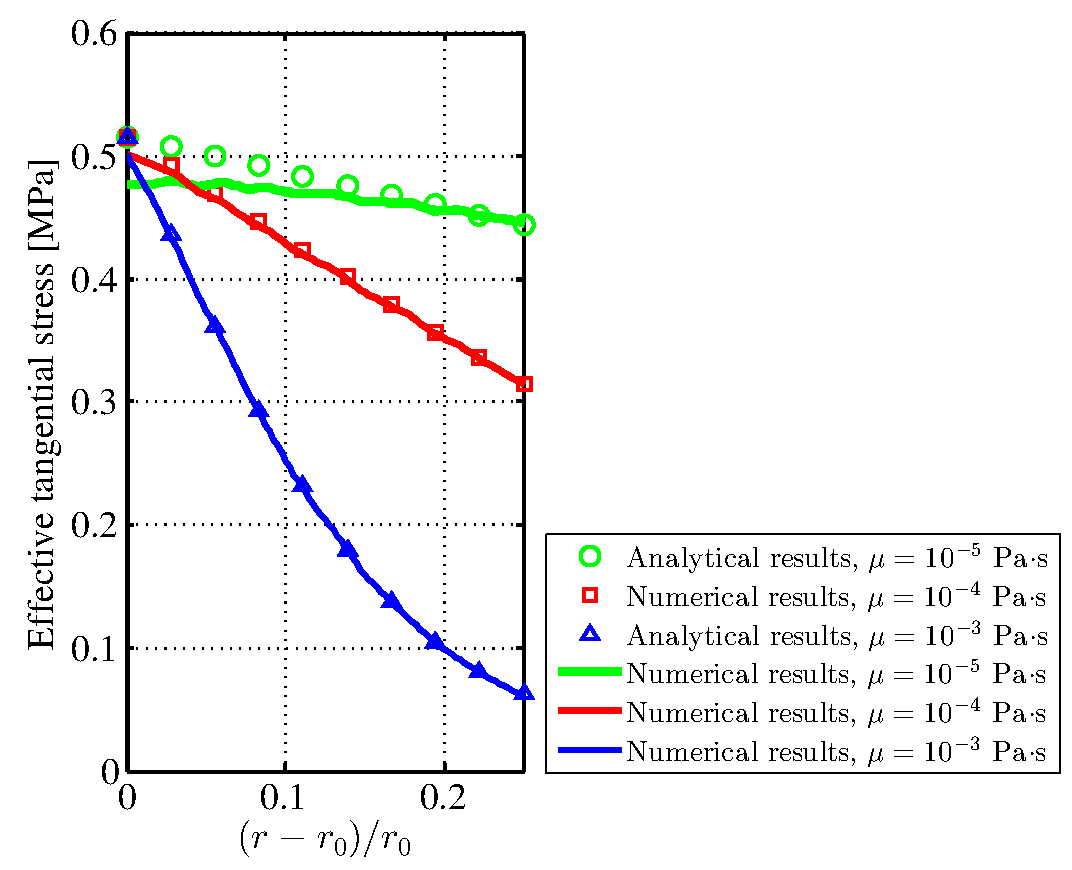
\includegraphics[width=0.8\textwidth]{verify_tangentialstress}
    \caption{Poroelastic response of a borehole. The effective tangential stress is plotted near the borehole for three different dynamic viscosities $\mu$ at early time $t=0.1$ s.}
    \label{Fig:Borehole_tangential_stress}
\end{figure}

\subsection{Computation of the crack opening displacement}
We now focus on a classical problem first solved by Sneddon and Lowengrouo \cite{SneddonLowengrub69} (see also \cite{bourdin2012variational}) that solves the opening displacement of a static line crack.

Consider a computational domain of $\Omega=4$ m $\times 4$ m with a preexisting line fracture of length $2a_0=0.4$ m, i.e., $\mathcal{C}=[1.8, 2.2]\times\{0\}$. To minimize the effect of the boundary conditions on the results, the domain size is much larger than the crack length ($L\gg 2a_0$).

The mechanical properties of the material are the Young's modulus $E=1000$ MPa, the Poisson's ratio $\nu=0$, and the fracture toughness $g_c=1$ MPa$\cdot$s.

We impose zero displacements on the external boundary of $\Omega$. Also we set $d=1$ on prescribed (initial) fracture and $d=0$ on the external boundary of $\Omega$. A monotonically increasing pressure is applied on the upper and lower faces of fracture with the magnitude $p=1$ MPa. Figure \ref{Fig:Sneddon_geometry} depicts the geometry and boundary conditions.

\begin{figure}
    \centering
    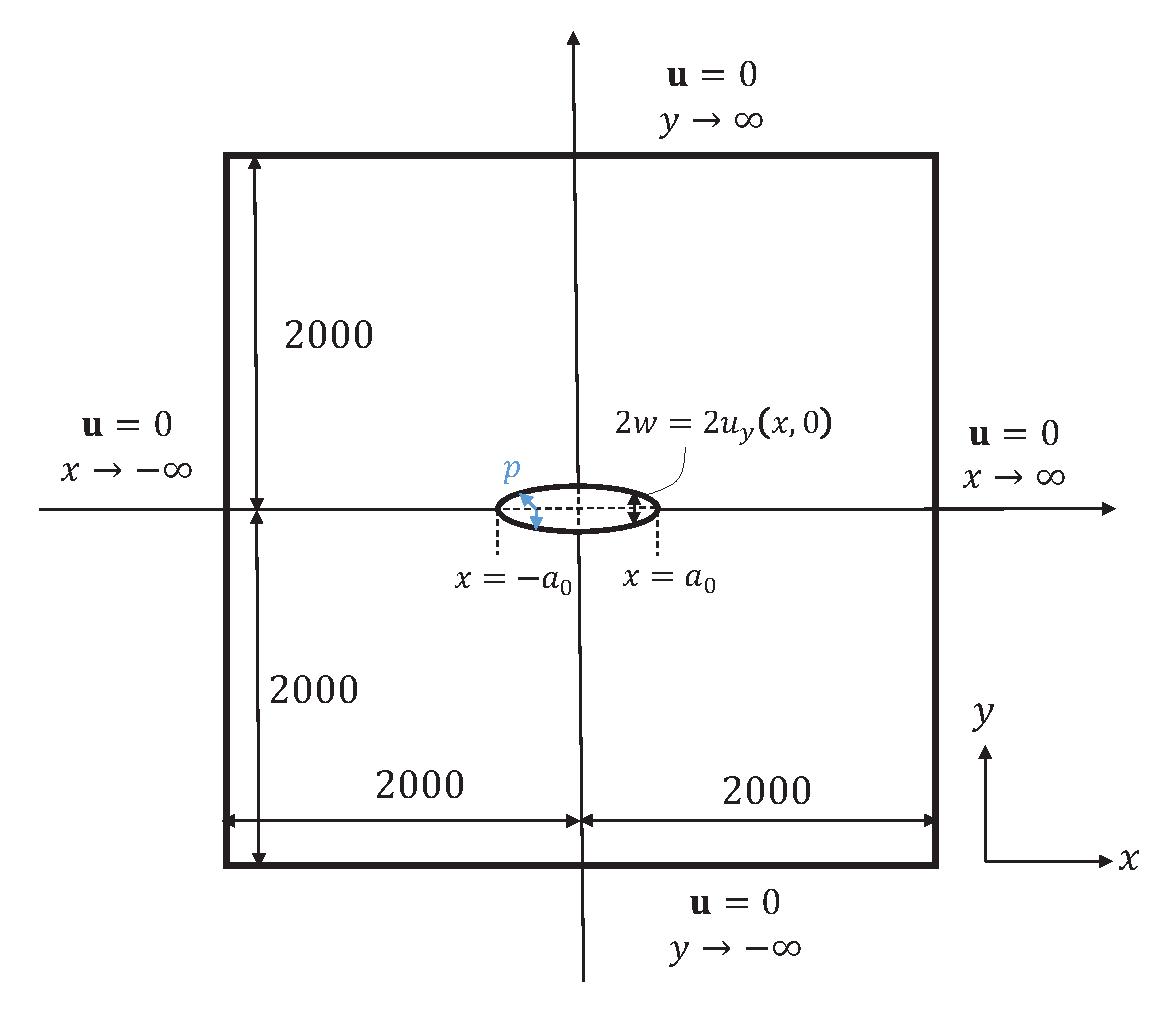
\includegraphics[width=0.8\textwidth]{centerCrack_sneddon.eps}
    \caption{Computation of the crack opening displacement. Schematic view of the deformed line crack in a two dimensional domain.}
    \label{Fig:Sneddon_geometry}
\end{figure}

%\todo{Mostafa: rewrite this part, these two paragraphs are a part of a PhD theses. \cite{Chukwudozie-2016a}}
 
%\paragraph*{Sneddon's 2D benchmark with constant pressure.}  This section simulates the deformation of a static line crack in an infinite two dimensional domain. This is the classic problem solved by Sneddon and Lowengrub (1969). The material is composed of a homogeneous isotropic. The domain is under plain strain conditions and the boundary conditions on the material is such that displacement and stresses vanish at infinity while the crack surface is acted upon by a uniform pressure p.  For the condition where the crack is found in the region defined by $y = 0$, $-l_0\le x \le l_0$, Sneddon and Lowengrub (1969) derived the following analytical expression for the crack opening displacement in the y-direction.
%\begin{equation} \label{eq: sneddon_opening}
%u_y(x,0)= \dfrac{2(p-\sigma_0) l_0}{E'}\sqrt{1-\dfrac{x_0}{l_0}}
%\end{equation}
%where $E'=\dfrac{E}{1-\nu^2}$. The fracture displacement profile is elliptic as evident from Equation \eqref{eq: sneddon_opening}. Thus, the fracture
%\begin{equation*}
% V_f=\pi \dfrac{2(p-\sigma_0) l_0^2}{E'}
%\end{equation*}

%\paragraph*{Compute the fracture width and volume.}  
Bourdin \emph{et al.}~\cite{BourdinCFRAC13} proposed a formula to compute the fracture aperture as:
\begin{equation*}
    w=\mathbf{u}\cdot n_{\Gamma} \simeq \int_{s} \mathbf{u} \cdot \nabla d \, dx.
\end{equation*}
Then, the fracture volume is calculated by integrating the fracture aperture along the fracture's path:
\begin{equation*}
    V_f= \int_{\Gamma} w \, ds \simeq \int_{\Omega} \mathbf{u} \cdot \nabla d \, d\Omega.
\end{equation*}

Figure \ref{Fig:Sneddon_opening} shows the {aperture} profile for different $h$ and $\ell$. The dash line in black represents the Sneddon's analytical solution \cite{SneddonLowengrub69}. Also, the crack volume computed by Sneddon's analytical solution and our numerical tests are summarized in Table \ref{Tab:Sneddon_volume}. %\todo{YS: Any conclusion?}

\begin{figure}[htbp]
    \centering
    \subfloat[]{
    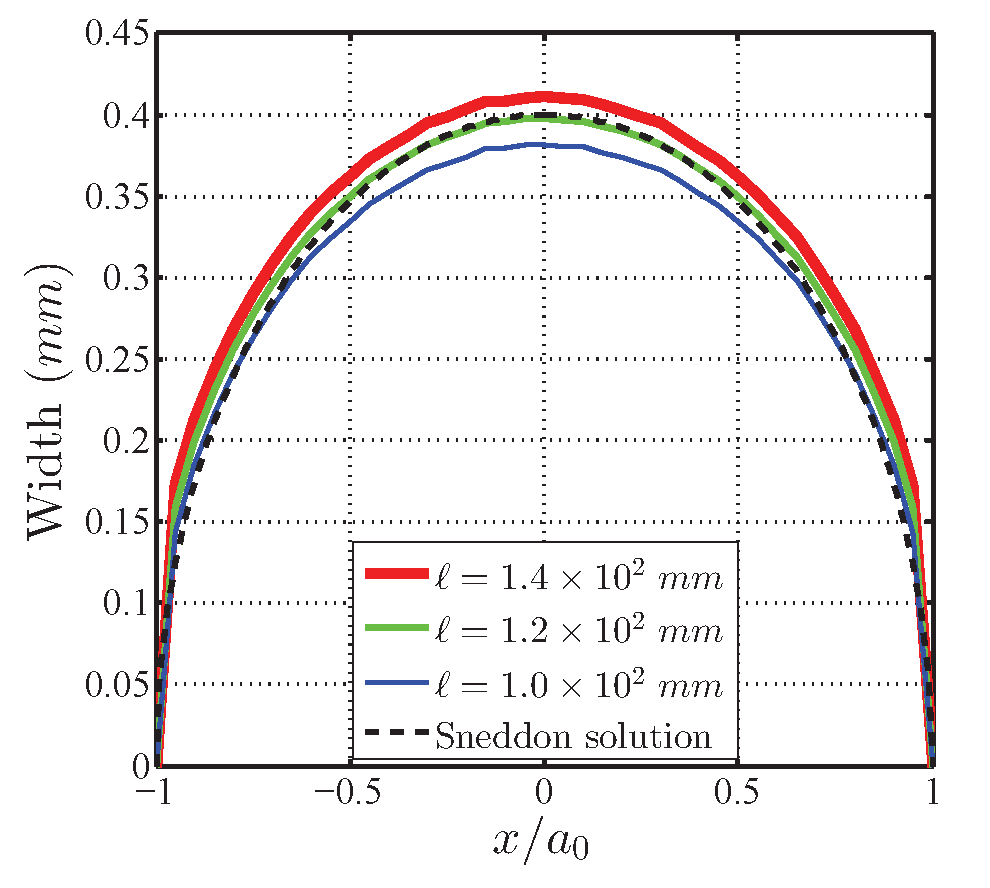
\includegraphics[width=0.5\textwidth]{width_ellVary.eps}
    \label{Fig:Sneddon_opening_ell}}
    \subfloat[]{
    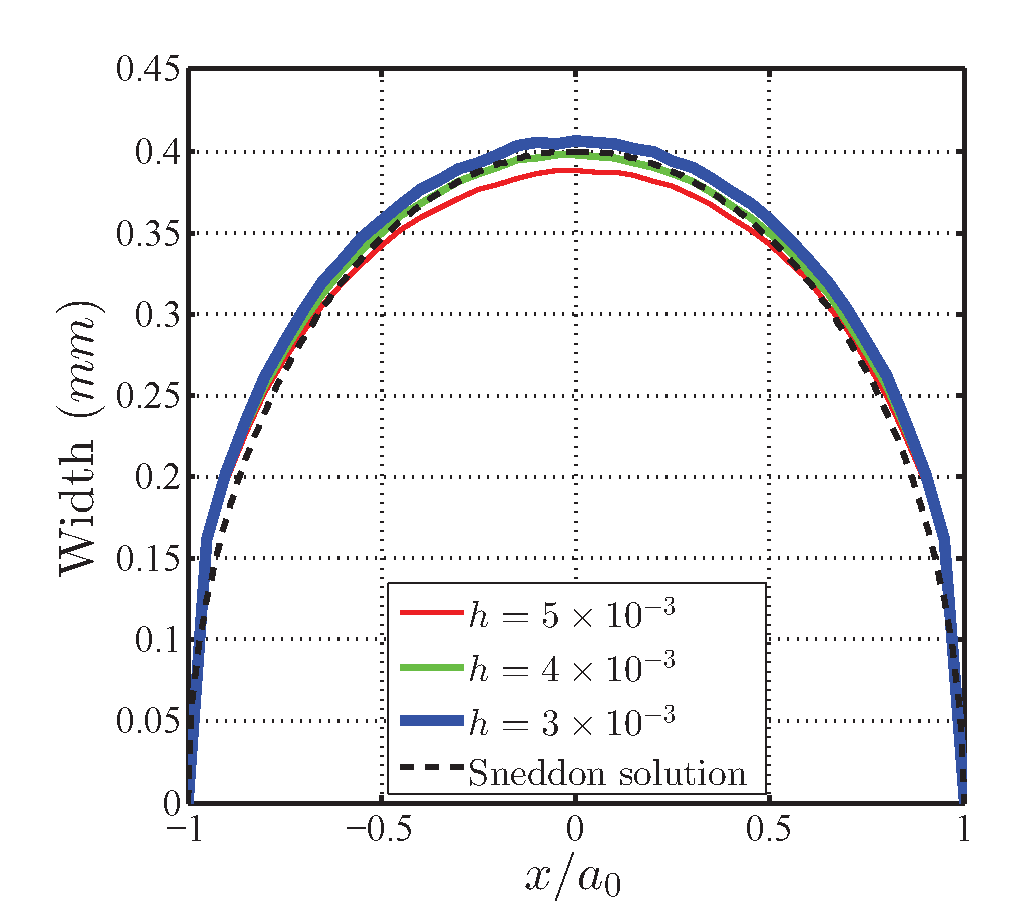
\includegraphics[width=0.5\textwidth]{width_hVary.eps}
    \label{Fig:Sneddon_opening_h}}    
    \caption{Computation of the crack opening displacement. We output the results for (\ref{Fig:Sneddon_opening_ell}) various $\ell$ with $h=4$ mm and (\ref{Fig:Sneddon_opening_h}) various $h$ with $\ell=1.2\times 10^{2}$ mm, and compare them with Sneddon's analytical solution \cite{SneddonLowengrub69}.}
    \label{Fig:Sneddon_opening}
\end{figure}

%\begin{figure}[htbp]
   % \centering
   % \includegraphics[width=0.7\textwidth]{centerCrackOpening.eps}
   % \caption{Phase field profile for center pressurized fracture, where $h=5  \times 10^-3~ \text{mm}$ and $\ell=4h$. }
 %   \label{Fig:opening_Pressrized_fracture_i}
%\end{figure}

\begin{table}[]
    \centering
    \caption{Crack volumes for different $\ell$ for numerical tests and analytical solution ($h=4\text{mm}$).}
    \begin{tabular}{l  c c c}
    \hline 
         $\ell$ (mm)  &1.4$\times 10^{2}$ & 1.2$\times 10^{2}$ &1.0$\times 10^{2}$\\
    \hline 
         Numerical fracture volume (mm$^2$) & 2.89$\times 10^{2}$ & 2.75$\times 10^{2}$  & 2.60$\times 10^{2}$\\
         Analytical fracture volume (mm$^2$) &2.51$\times 10^{2}$\\
    \hline      
    \end{tabular}
    \label{Tab:Sneddon_volume}
\end{table}
\section{Weak forms {and discretized formulations}}\label{sub:weak_form}
Here we provide weak forms useful for FEniCS implementation. \added{For more information on implementing the phase field approach for fracture, see \cite{shen2018implementation}.}

\subsection{Porous medium} \label{sub:weak_porous}
To proceed, let the test function spaces be
\begin{equation*}
    \begin{aligned}
        \mathscr{V}_u &:= \left\{\bar{\bm{u}}\in H^1\left(\Omega; \mathbb{R}^2\right) \middle|
        \bar{\bm{u}} = \mathbf{0} \quad \text{on} \quad\Gamma_D
        \right\},\\
        \mathscr{V}_d &:= H^1(\Omega).
    \end{aligned}
\end{equation*}
%\todo[inline]{YS: It may look better by writing \eqref{Eq:Residual} as two equations, one obtained by taking the first variation of $\bm{u}$ and the other of $d$.\\
%Mostafa: Done}
Then we derive the first variations of the energy functional \eqref{Eq:Dissipative_functional}, which will be needed for stating the weak form:
\begin{subequations} \label{Eq:Residual}
    \begin{align}
	    \begin{split}
	    \label{Eq:Residual_u}\delta \Pi_\ell & \left[(\bm{u}, d); \bar{\bm{u}} \right]
	    := \int_\Omega \bm{\sigma}[\bm{\varepsilon}(\bm{u}), d] : \bm{\varepsilon}(\bar{\bm{u}}) \;d\Omega - \int_{\Gamma_N} \bm{t}_N\cdot \bar{\bm{u}} \; d\Gamma - \int_\Omega \bm{b} \cdot\bar{\bm{u}}\; d\Omega \\
	    &+\int_{\Omega} \left(\alpha-1\right) \nabla \left((1-d)^2  {p}\right) \cdot \bar{\bm{u}} \; d\Omega + \int_{\Omega}  {\left(1 - d\right)}^2\nabla {p}\cdot \bar{\bm{u}}  \; d\Omega
	    \end{split}\\
	    \begin{split}
	     \label{Eq:Residual_d}\delta \Pi_\ell & \left[(\bm{u}, d);  \bar{d} \right]
	    	    := \int_{\Omega} \left(\alpha-1\right)g'(d)\bar{d} {p} \divergence{\bm{u}} \; d\Omega +	\int_{\Omega} g'(d)\bar{d}   \nabla {p} \cdot {\bm{u}} \; d\Omega 
        \\
	    & + \int_\Omega g'(d) \psi_+(\bm{\varepsilon}) \bar{d}  \; d\Omega +
	    \frac{g_c}{4c_w} \int_\Omega  \left(\frac{\omega'(d)\;\bar{d}}{\ell} + 2\ell \nabla d\cdot\nabla \bar{d} \right)\;d\Omega.
	    \end{split}
	\end{align}
\end{subequations}
The weak form can thus be stated as: Find $\left(\bm{u}\times d \right)\in\mathscr{S}_{\bm{u}}\times\mathscr{S}_d$, such that for all admissible functions $\left(\bar{\bm{u}}\times\bar{d} \right)\in\mathscr{V}_{\bm{u}}\times\mathscr{V}_d$, $\delta\Pi_\ell\left[(\bm{u},d); \bar{\bm{u}}\right]=0$ and $\delta\Pi_\ell\left[(\bm{u},d); \bar{d}\right]=0$.


%\todo[inline]{YS: The second variation should also be written as two expressions, $ \delta^2 \Pi_\ell \left[(\bm{u}, d); \bar{\bm{u}}, \delta \bm{u}\right]$ and $\delta^2 \Pi_\ell \left[(\bm{u}, d); \bar{d}, \delta d\right]$, because we are doing a staggered algorithm.}
Also we take another variation from \eqref{Eq:Dissipative_functional} which will be needed for the discretized formulation:
\begin{subequations}\label{Eq:Tangent}
\begin{align}\label{Eq:Tangent_u}
\begin{split}
        \delta^2 \Pi_\ell & \left[(\bm{u}, d); \bar{\bm{u}}, \delta \bm{u}\right]
        = \int_\Omega \bm{\varepsilon}(\delta\bm{u}): \mathbb{C}[\bm{\varepsilon}(\bm{u}), d] : \bm{\varepsilon}(\bar{\bm{u}})  \;d\Omega,
        \end{split}\\
        \begin{split}
	            \delta^2 \Pi_\ell & \left[(\bm{u}, d);  \bar{d},  \delta d\right]
	    =  \int_\Omega \delta d \;g''(d) \psi_+(\bm{\varepsilon}) \bar d \; d\Omega\\ 
	    & +\int_{\Omega} \left(\alpha-1\right) g''(d)\bar{d} \; \delta d \; {p} \divergence {{\bm{u}}} \; d\Omega +\int_{\Omega}  g''(d)\bar{d} \; \delta d \; \nabla {p} \cdot {{\bm{u}}} \; d\Omega 
	    \\& +
	    \frac{g_c}{4c_w} \int_\Omega  \left[\frac{\delta d \; w''(d) \bar{d}}{\ell} + 2\ell \nabla (\delta d) \cdot \nabla \bar d \right]\;d\Omega,
	    \end{split}
\end{align}
\end{subequations}
where the fourth-order tensor $\mathbb{C}[\bm{\varepsilon}(\bm{u}), d] = \left.\frac{\partial \bm{\sigma}(\bm{\varepsilon}, d)}{\partial \bm{\varepsilon}}\right|_{\bm{\varepsilon}=\bm{\varepsilon}(\bm{u})}$ is the tangent elasticity tensor.

%\todo[inline]{YS: It looks like we don't need the following content until the beginning of Section \ref{sec:CO2-discretization}.\\
%	YS: After discussing with Mostafa on October 4, I think a better idea is, since we are using FEniCS, to keep the weak form and Jacobian in an appendix, and remove equations like \eqref{Eq:discretization} and \eqref{Eq:p_discretized}, and also remove \eqref{Eq:Residual_disc} and also the matrix formulations after it.\\Vahid: If I understood you correctly, you mean we do not need the entire subsection named ``Spatial discretization of porous medium'' \ref{sub:spatial_porous} anymore, right? I still kept the material in the tex file, and the title here though. I also changed \ref{sec:CO2-discretization} according to your comment.}
%\subsubsection{Spatial discretization of porous medium}\label{sub:spatial_porous}
%%\todo[inline]{YS: If we use a triangular mesh, then the shape functions cannot be $Q_1$.\\
%%Vahid: Yes. $Q_1$ is omitted now.}
{To discretize the problem, we divide $\Omega$ with a conforming mesh $\mathscr{T}_h$ of triangular elements. % for two dimensions, each member characterized by the mesh size $h$. 
Let $\eta$ be the set of nodes of $\mathscr{T}_h$. We approximate $(\bm{u},d)$ with the standard {$P_1$} finite element basis functions associated with all nodes $i \in\eta$:}
\begin{equation}\label{Eq:discretization}
    \begin{aligned}
        \bm{u}(\bm{x})=\sum_{i\in\eta} \bm{N}^{\bm{u}}_{i}(\bm{x}) \mathbf{u}_i,\quad
	    d(\bm{x})=\sum_{i\in\eta}N_i(\bm{x}) d_i,
	\end{aligned}
\end{equation}
{where $\mathbf{u}_i$, and $d_i$ are the displacement and phase field values at node $i$, respectively; and $\bm{N}^{\bm{u}}_{i}$ is given by:}
\begin{equation*}
    \begin{aligned}
        \bm{N}^{\bm{u}}_{i}=\left[
		\begin{array}{c c}
			N_i &  0 \\
			0 & N_i
		\end{array}
		\right],
    \end{aligned}
\end{equation*}
{where $N_i$ is the standard finite element shape function associated with $i\in\eta$, satisfying $N_j(\mathbf{x}_i)=\delta_{ji}$, for all $i,j\in\eta$, and $\mathbf{x}_i,\mathbf{u}_i\in\mathbb{R}^{2}$ are the position vector and nodal displacement vector of node $i$, respectively. %The sets $\eta_D,\eta_d \subset \eta$ denote the sets of nodes at which $\bm{u}$ and $d$ are prescribed, respectively.
%	on  $\Gamma_D$, i.e., if $i\in\eta_D$, $\mathbf{u}_i = \bm{u}_D(\mathbf{x}_i)$. The unknowns to solve are thus $\mathbf{u}_i$ for $i\in\eta\setminus\eta_D$, and $d_i$ for all $i\in\eta$. 
Note that we also apply the same discretization to the test functions.}

\paragraph{Discretized weak form} {Let $n_\text{nodes}$ denote the number of nodes in $\eta$.
	Let $\mathbf{u}\in\mathbb{R}^{2n_\text{nodes}}$, $\mathbf{d}\in\mathbb{R}^{n_\text{nodes}}$ contain all entries of $\mathbf{u}_i$, ${d}_i$, respectively, for all $i\in\eta$. The discretized residuals can be written as $\mathbb{U}_i (\mathbf{u}):= \delta \Pi (\bm{u}; \bm{N}_i^{\bm{u}})\in\mathbb{R}^2$ and $\mathbb{D}_i({d}):=\delta\Pi ({d}; {N}_i)\in\mathbb{R}$ for all $i\in\eta$. %, where $\mathbf{R}_A$. 
With \eqref{Eq:Residual}, these residual vectors are expressed as follows:}
\begin{equation}\label{Eq:Residual_disc}
	\begin{aligned}
		\mathbb{U}_i & = \int_\Omega (\bm{B}_i)^T \bm{\sigma}[\bm{\varepsilon}(\bm{u}), d] \;d\Omega - \int_{\Gamma_N} (\bm{N}^{\bm{u}}_{i})^T\bm{t}_N \; d\Gamma - \int_\Omega (\bm{N}^{\bm{u}}_{i})^T\bm{b} \; d\Omega\\ &\quad +\int_{\Omega} (\alpha-1)(\bm{N}^{\bm{u}}_{i})^T \nabla\left((1-d)^2 {p}\right) \; d\Omega +\int_{\Omega}  (\bm{N}^{\bm{u}}_{i})^T {\left(1 - d\right)}^2\nabla {p} \; d\Omega\\
	    \mathbb{D}_i &= \int_{\Omega} \left(\alpha-1\right)g'(d)N_i \;{p} \divergence \bm{u} \; d\Omega + \int_{\Omega} g'(d) N_i (\nabla {p})^T  \bm{u} \; d\Omega \\
	    & \quad+\int_\Omega g'(d) \psi_+(\bm{\varepsilon}) N_i \; d\Omega + \frac{g_c}{4c_w} \int_\Omega  \left(\frac{w'(d) N_i}{\ell} + 2\ell \nabla d \cdot \nabla N_i \right)\;d\Omega,
	\end{aligned}
\end{equation}
{where $\mathbb{U}_i$ is also called the nodal force at $i$. % obtained with displacement test function and phase field test function
Also note that in \eqref{Eq:Residual_disc}, $\bm{\sigma}$ is understood as a 3-vector, % in 3D.
and the strain-displacement matrix for node $i$ are given by:}
\begin{equation*}
    \bm{B}_i=\left[
	\begin{array}{c c}
 	N_{i,x} &  0\\
 	0 & N_{i,y} \\
 	N_{i,y} & N_{i,x} \\
 	\end{array}
 	\right].
\end{equation*}
{The discretized weak form is $\mathbb{U}_i=\mathbf{0}$ for all nodes $i$ at which $\bm{u}$ is not prescribed, and $\mathbb{D}_i=0$ for all nodes $i$ at which $d$ is not prescribed.
}
%
\paragraph{Tangent stiffness matrices} {The tangent stiffness matrices are needed for Newton-Raphson algorithms. The tangent stiffness matrix components of \eqref{Eq:Tangent} are $\mathbf{K}_{ij}^u:=\partial\mathbb{U}_i/\partial\mathbf{u}_j=\delta^2\Pi[\bm{u};\bm{N}^{\bm{u}}_i, \bm{N}^{\bm{u}}_j]\in \mathbb{R}^{2\times 2}$ for all $i,j\in\eta$ and $ K_{ij}^d :=\partial\mathbb{D}_i/\partial {d}_j=\delta^2\Pi[{d};{N}_i, {N}_j]\in \mathbb{R}$ for all $i,j\in\eta$, which can be expressed as follows:}
\begin{subequations}
    \begin{align}
        \mathbf{K}_{ij}^u &= \int_\Omega (\bm{B}_i)^T \mathbf{D} \bm{B}_j \;d\Omega,\\
    \begin{split}
        K_{ij}^d &= \int_{\Omega} \left(\alpha-1\right)g''(d)N_iN_j \;{p} \divergence \bm{u} \; d\Omega 
        + \int_{\Omega} g''(d) N_i N_j (\nabla {p})^T \bm{u} \; d\Omega 
	    \\ &+
	    \int_\Omega \;g''(d) \psi_+(\bm{\varepsilon}) N_i N_j\; d\Omega + \frac{g_c}{4c_w} \int_\Omega \left[\frac{w''(d) N_i \; N_j}{\ell} + 2\ell (\nabla N_i)^T \nabla N_j \right]d\Omega,
    \end{split}
    \end{align}
\end{subequations}
{where we denote by $\mathbf{D}$ the matrix form of the tangent elastic modulus tensor $\mathbb{C}$. Below we give its expression $\mathbf{D}=g(d)\mathbf{D}_++\mathbf{D}_-$ for our adopted tension-compression decomposition \cite{Amor09}:}
%\paragraph{Model A} We have $\mathbf{D}_+=\mathbf{D}_0$ and $\mathbf{D}_-=\mathbf{0}$ 
%where $\mathbf{D}_0$ for the plane strain case is defined as:
%\begin{equation*}\label{Eq:D_0}
%	    \bm{D}_{0} = \begin{bmatrix} 
%	    \lambda+2\mu & \lambda & 0 \\
%	    \lambda & \lambda+2\mu & 0 \\
%	    0 & 0 & \mu
%	   \end{bmatrix}.
%\end{equation*}
% 
%\added{Let $\mathbf{1}$ be the $3\times3$ identity matrix. Then}
\[\begin{aligned}
\mathbf{D}_+ &= BH(\trace\bm{\varepsilon}) \begin{bmatrix}
1 & 1 & 0 \\
1 & 1 & 0 \\
0 & 0 & 0 
\end{bmatrix} + \frac{G}3 \begin{bmatrix}
4 & -2 & 0 \\
-2 & 4 & 0 \\
0 & 0 & 3 
\end{bmatrix} ,\\
\mathbf{D}_- &= BH(-\trace\bm{\varepsilon}) \begin{bmatrix}
1 & 1 & 0 \\
1 & 1 & 0 \\
0 & 0 & 0 
\end{bmatrix},
\end{aligned}\]
%\[\begin{aligned}
%\mathbf{D}_+ &= BH(\trace\bm{\varepsilon}) \begin{bmatrix}
%1 & 1 & 0 \\
%1 & 1 & 0 \\
%0 & 0 & 1 
%\end{bmatrix} + \frac23G\begin{bmatrix}
%2 & -1 & 0 \\
%-1 & 2 & 0 \\
%0 & 0 & 2 
%\end{bmatrix} ,\\
%\mathbf{D}_- &= BH(-\trace\bm{\varepsilon}) \begin{bmatrix}
%1 & 1 & 0 \\
%1 & 1 & 0 \\
%0 & 0 & 1 
%\end{bmatrix},
%\end{aligned}\]
%\[\begin{aligned}
%\mathbf{D}_+ &= KH(\trace\bm{\varepsilon}) \begin{bmatrix}
%1 & 1 & 0 \\
%1 & 1 & 0 \\
%0 & 0 & 1 
%\end{bmatrix} + 2\mu\left(\mathbf{1} - \frac13\begin{bmatrix}
%1 & 1 & 0 \\
%1 & 1 & 0 \\
%0 & 0 & 1 
%\end{bmatrix} \right),\\
%\mathbf{D}_- &= KH(-\trace\bm{\varepsilon}) \begin{bmatrix}
%1 & 1 & 0 \\
%1 & 1 & 0 \\
%0 & 0 & 1 
%\end{bmatrix} .
%\end{aligned}\]
{where $B=E/[3(1-2\nu)]$ is the bulk modulus.
	Here, $H$ is the Heaviside function such that $H(a)=1$ if $a>0$, $H(a)=0$ if $a<0$, and $H(a)=\frac12$ if $a=0$.}

%\subsection{Compressible (CO$_2$) fluid flow}

\subsection{Compressible (CO$_2$) fluid flow discretization}
\label{sec:CO2-discretization}
The compressible fluid flow discretization is also done via the finite element method. We first discretize in time and then in space. We will adopt the backward Euler method for time discretization.

%\todo[inline]{YS: The same time steps or no?\\
%Vahid: Yes, the same time step. Look the changed sentence below in blue for the changes.\\
%YS: No! We cannot first introduce the discrete times and then after a few lines we say they are equally spaced. If they are equally spaced, then we say that up front! We first decide on the number of time steps, and then the discrete times and the time step are determined.\\
%Vahid: All parts are removed now.\\
%Another point: The notation $N$ is conflicted.\\
%Vahid: All parts are removed now.}
%\todo[inline]{YS: I suggest we keep $k(d)$ all along, instead of writing $k_0\exp(7d)$, to leave flexibility in the choice of the model.\\
%Vahid: OK. Now the relevant equation \eqref{Eq:weak_pressure} is modified.}
%\paragraph{Time discretization}
%\replaced{hi}{We choose $0=t_0<t_1<\ldots<t_N=\replaced{t_f}{T}$ and seek the solution at these discrete instants. We will adopt the backward Euler method for time discretization. Now we detail how we advance from time step $n-1$ to $n$. For later convenience, let $\Delta t_n := t_n - t_{n-1}$ for $n=1,\ldots,N$. \added{As we use the same time steps,} when there is no risk of confusion, the subscript $n$ will be dropped. \replaced{It implies}{Moreover,} the field $p$ will wear a superscript $n-1$ if it refers to the solution at $t_{n-1}$, but will have no superscript if it refers to the solution at the current time step, i.e., $t_n$.} With this specific, \eqref{Eq:General_pressure} is discretized as:

%\begin{equation} \label{Eq:General_pressure_time_discrete}
 %   \begin{aligned}
  %      \frac{\phi}{{N}}\frac{ p-p^{n-1}}{\Delta t}+\rho \dfrac{ \varepsilon_v-\varepsilon_v^{n-1}}{\Delta t}
%		\added{-\frac{1}{\mu}\left[\frac{k}{N}\left|\nabla p\right|^2+k\rho\Delta p+\rho\nabla k\cdot \nabla p\right]}=Q_g \; \;on \;\Omega,
%    \end{aligned}
%\end{equation}
%\Comment{YS: The equation $p \in H^1(\Omega; \mathbb{R})$ should read $p \in H^1 (\Omega)$}

%\todo[inline]{YS: Mostafa, this paragraph is taken from our previous paper. Now we are solving EQUATIONS instead of inequalities, then there is no need to say ``necessary condition.''\\Mostafa: Right. It's deleted.}
%\todo[inline]{YS: How come we have $\Gamma_B$? Is it part of $\partial \Omega$? This should have appeared in Section \ref{sec:Math_model}.\\Vahid: The related part is removed now. We have defined $\Gamma_B$ in Section \ref{sec:Math_model}.}
%\todo[inline]{YS: Why do we use $\delta p$ here but $\overline{\bm{u}}$ and $\overline{d}$? It looks like the latter is better as $\delta$ is also used in the EOS.\\Vahid: Now I changed it to $\overline{p}$.}
%\paragraph{Spatial discretization}
%Let the admissible {set} of pressure be
%\begin{equation*}
%    \begin{aligned}
%        \mathscr{S}_p &:= \left\{p \in H^1 (\Omega) \middle|
%        p = p_D\text{ on }\Gamma_D \right\}.
%    \end{aligned}
%\end{equation*}
%\todo[inline]{YS: Move $\mathscr{S}_p$ here. Again, make sure on which part of $\partial\Omega$ we are imposing $p$.\\Vahid: Done. Now we are imposing $p_D$ on $\Gamma_P$.}

To proceed, let the admissible set of pressure be:
\begin{equation*}
	\mathscr{S}_p := \left\{p \in H^1 (\Omega) \middle|
	p = p_D\quad\text{on}\quad\Gamma_P \right\}.
\end{equation*}
The test function space can be defined as:
\begin{equation*}
\mathscr{V}_{p}:= \left \{{\overline{p}}\in H^1(\Omega) \middle | {\overline{p}} =0 \quad \text{on} \quad \Gamma_P \right \}.
\end{equation*}
The weak form can be stated as: find $p\in\mathscr{S}_p$ such that for all admissible functions $\overline{p}\in\mathscr{V}_p$,
\begin{equation}\label{Eq:weak_pressure}
\begin{aligned}
        & \frac{1}{\Delta t} \int_{\Omega} {\phi}(\rho-\rho^{n-1}) {\overline{p}} \; d\Omega + \dfrac{1}{{\Delta t}}\int_{\Omega} \rho(\varepsilon_v-\varepsilon_v^{n-1}) {\overline{p}} \; d\Omega \\& +  \int_{\Omega} \rho \frac{k(d)}{\mu} \nabla p \cdot \nabla {\overline{p}} \; d\Omega   
                  -\int_{\Gamma_B} Q_g {\overline{p}} \; d\Gamma =0,
\end{aligned}
\end{equation}
where $\rho^{n-1}$ and $\varepsilon_v^{n-1}$ denote solutions at the previous time step.
 %where $\Gamma_B$ is the boundary of borehole. %Also, the third term of the above equation is obtained by integration by parts:

%\begin{equation}\label{Eq:dis_div}
%\begin{aligned}
%        & \frac{1}{\mu} \int_{\Omega} k(d)\rho \;\Delta p \; d\Omega=\\&- \frac{1}{\mu} \int_{\Omega}  {k(d)}\rho \; \nabla p \cdot \nabla {\overline{p}} +   \frac{1}{\mu} \int_{\Gamma_N} k(d)\rho\;\nabla p \cdot \bm{n} \; d\Gamma %+   \frac{1}{\mu} \int_{\mathcal{C}} k(d)\rho\;\nabla p \cdot \bm{n} \; d\Gamma
%\end{aligned}
%\end{equation}

{Also, we {use} %\todo{YS: serve?} 
the conventional finite element shape functions $\{N_i\}$ for $p$:}
\begin{equation}\label{Eq:p_discretized}
\begin{aligned}
	    p(\bm{x})=\sum_{i\in\eta} p_i N_i(\bm{x}).
\end{aligned}
\end{equation}
{Thus, the residual vector form of \ref{Eq:weak_pressure} is expressed as follows:}
\begin{equation}\label{Eq:flow_weak}
\begin{aligned}
      \mathbb{P}_i := &  \frac{1}{\Delta t} \int_{\Omega} {\phi}(\rho-\rho^{n-1}) {N_i} \; d\Omega + \dfrac{1}{{\Delta t}}\int_{\Omega} \rho(\varepsilon_v-\varepsilon_v^{n-1}) {N_i} \; d\Omega \\& +  \int_{\Omega} \rho \frac{k(d)}{\mu} (\nabla p)^T \nabla {N_i} \; d\Omega   
                        -\int_{\Gamma_B} Q_g {N_i} \;d\Gamma.
\end{aligned}
\end{equation}
{The discretized weak form is $\mathbb{P}_i=0$ for all nodes $i$ at which $p$ is not prescribed.}

{The tangent stiffness matrix form of the fluid flow $K_{ij}^p:=\partial\mathbb{P}_i/\partial{p}_j$ %\in \mathbb{R}$ 
for all $i,j\in\eta$, which can be expressed as follows:}
\begin{equation}\label{Eq:flow_stiff}
      K_{ij}^p :=    \int_{\Omega} \rho \frac{k(d)}{\mu} (\nabla N_i)^T  \nabla {N_j} \; d\Omega.
\end{equation}


\section*{Acknowledgments}
  This work is supported by the National Natural Science Foundation of China with grant \#11402146. YS also acknowledges the financial support by the Young 1000 Talent Program of China.

%\section*{References}
%% Vancouver name/year
%\bibliographystyle{model4-names}\biboptions{authoryear}
\bibliography{ref}

\end{document}